\documentclass[ordinary]{BMSTU-IU8}

\usepackage{amsfonts}
\usepackage{stmaryrd}
\usepackage{amssymb}

\addbibresource{main.bib}

\group{ИУ8-104}
\theme{Выводы об оценке сложности протоколов безопасности
       на основе возведения в степень по схеме Диффи–Хеллмана
       и коммутируемого шифрования с открытым ключом}
\discipline{Криптографические методы защиты информации}
\student{Мильченко И. Д.}
\supervisor{Жуков А. Е.}

\begin{document}
  \maketitle

  \tableofcontents

  \introduction

В современном мире обработки данных отказоустойчивость и надежность распределенных
систем являются ключевыми требованиями для множества приложений, начиная от облачных
сервисов и заканчивая базами данных и системами хранения информации. Одним из
фундаментальных механизмов, обеспечивающих согласованность данных в распределенных
системах, является алгоритм консенсуса. Среди различных алгоритмов консенсуса, таких
как Paxos, Viewstamped Replication и другие, алгоритм Raft выделяется своей простотой
понимания, формальной доказанностью корректности и эффективностью работы.

Raft представляет собой алгоритм консенсуса, предназначенный для управления
распределенными системами и поддержания согласованности реплицированных логов.
Он был предложен Диего Онгаро и Джоном Оустером в 2014 году \cite{ongaro2014raft} как более понятная
альтернатива Paxos, что делает его привлекательным для реализации в практических
системах.

В рамках данной научно-исследовательской работы рассматривается задача создания
отказоустойчивого распределенного хранилища данных на основе алгоритма Raft. В первой
части работы проводится анализ существующих реализаций Raft, обосновывается выбор одной
из библиотек для репликации данных, а также разрабатывается архитектура хранилища с
учетом интеграции данной библиотеки. Кроме того, рассматриваются механизмы взаимодействия
узлов для достижения консенсуса и обеспечения надежности системы.

Во второй части работы будет осуществлена реализация основных операций хранилища,
включая механизм репликации данных, а также проведено тестирование системы на предмет
отказоустойчивости.

Таким образом, цель данной работы заключается в проектировании и разработке
распределенного хранилища данных, использующего алгоритм Raft для обеспечения
согласованности и высокой доступности данных.


  \section{Протокол и модель злоумышленника}

Модель протокола и злоумышленника, которую мы описываем далее, расширяет стандартные модели для (автоматического) анализа протоколов безопасности
\cite{Amadio2002} в двух отношениях. Во-первых, сообщения могут строиться с помощью
оператора $Exp(\cdot,\cdot)$, означающего экспоненциацию, и оператора произведения "\(\cdot\)". Во‑вторых, помимо стандартных правил перезаписи
модели Долева–Яо, злоумышленник снабжён дополнительными «правилами-оракулами», которые будут конкретизированы правилами экспоненциации термов.
В дальнейшем мы приведём формальное определение нашей модели, задав терминологию для термов, сообщений, протоколов, злоумышленника и атак.

\subsection{Термины и сообщения}

Множество термов \textit{term} определяется следующей грамматикой:
\[
\begin{array}{rl}
  \mathit{term} ::= & \mathcal{A} \mid \mathcal{V} \mid (\mathit{term}, \mathit{term}) \mid \{\mathit{term}\}^{s}_{k_{\mathit{term}}} \\
                  & \mid \{\mathit{term}\}^{p}_{k} \mid \mathit{Exp}(\mathit{term}, \mathit{product}) \\
\mathit{product} ::= & \mathit{term}^{\mathbb{Z}} \mid \mathit{term}^{\mathbb{Z}} \cdot \mathit{product}
\end{array}
\]
где $\mathcal{A}$ — конечное множество констант (атомарных сообщений), включающее имена субъектов, случайные значения, ключи, и специальные
константы $1$ и секрет. Множество $\mathcal{K} \subseteq \mathcal{A}$ содержит все открытые и закрытые ключи. $\mathcal{V}$ — конечное
множество переменных, $\mathbb{Z}$ — множество целых чисел, используется для показателей в произведениях. Предполагается, что существует биекция
${.}^{-1} : \mathcal{K} \to \mathcal{K}$, сопоставляющая каждому открытому (закрытому) ключу $k$ соответствующий закрытый (открытый) $k^{-1}$.

Бинарный символ $\langle\cdot,\cdot\rangle$ обозначает объединение в пару, символ $\{\cdot\}^{s}$ используется для симметричного шифрования,
а символ $\{\cdot\}^{p}$ — для шифрования с открытым ключом. Заметим, что симметричный ключ может быть произвольным термом, в то время как для
шифрования с открытым ключом допускаются только атомарные ключи из $\mathcal{K}$.

Оператор произведения ``$\cdot$'' моделирует умножение в абелевой группе. Например, произведение $a^2 \cdot b^3 \cdot c^{-2}$ представляет элемент
этой группы, где $a^2 = a \cdot a$, $b^3 = b \cdot b \cdot b$, а $c^{-2} = c^{-1} \cdot c^{-1}$, причём $c^{-1}$ — обратный к $c$. В протоколе
A-GDH.2, к примеру, в качестве абелевой группы используется подгруппа $G$ порядка $q$ мультипликативной группы $\mathbb{Z}_p^*$, где $p$ и $q$
— простые числа. Термы и продукты рассматриваются с учётом коммутативности и ассоциативности оператора $\cdot$, а также с учётом тождества $t^1
= t$. Например, термы $d^1 \cdot c^{-2} \cdot (b^3 \cdot a^2) \quad \text{и} \quad a^2 \cdot b^3 \cdot c^{-2} \cdot d$ считаются представлениями
одного и того же продукта. Также, если мы пишем $t_1^{z_1} \cdots t_n^{z_n}$, то всегда предполагается, что ведущий символ $t_i$ не является
продуктом. Этого можно достичь, расставив скобки соответствующим образом. Мы используем обозначение $t_1^{z_1} \cdots t_n^{z_n}$ для обозначения
продукта, где $z_i$ — некоторые ненулевые целые числа. Оператор $\mathit{Exp}(\cdot,\cdot)$ означает возведение в степень. Например,
$\mathit{Exp}(a, b^2 \cdot c^{-1}) = a^{b^2 \cdot c^{-1}}$.

Если $t, t_1, \dots, t_n$ — термы и $n \geq 2$, то произведение вида $t^z$ (при $z \ne 1$) или вида $t_1^{z_1} \cdots t_n^{z_n}$ называется
\textit{нестандартным термом} (non-standard term). Мы часто обозначаем терм или продукт как \textit{терм}. Чтобы различать их, мы используем
понятие \textit{стандартного терма}, противопоставляя его нестандартному.

Переменные обозначаются $x,y,\dots$, а сами термы — $s,t,u,v$. 
Конечные множества термов пишем $E,F,\dots$ и их «украшенные» варианты.  
Для краткости будем записывать $E\cup F \;\text{как}\; E,F, \text{объединение} E\cup\{t\} \;\text{как}\; E,t, \text{и} E\setminus\{t\} \;\text{как}\; E\setminus t$.

Для терма $t$ и множества термов $E$ через $\mathcal{V}(t)$ и $\mathcal{V}(E)$ обозначим
соответственно множество переменных, встречающихся в $t$ и в $E$.

Наземный терм (или \emph{сообщение}) — это терм без переменных.
Термины \emph{стандартное} и \emph{нестандартное сообщение} употребляются
так же, как стандартный и нестандартный терм.  
\emph{(Наземная) подстановка} $\sigma$ — это отображение из $\mathcal V$ в множество
стандартных наземных термов.  Применение $\sigma$ к терму $t$ (или множеству $E$)
обозначается $t\sigma$ (соответственно $E\sigma$) и определяется обычным образом.

Скажем, что термы $t$ и $t'$ \emph{совпадают с точностью до показателей произведения}
(пишем $t\approx t'$), если они различаются только значениями степеней.  Например:
\[
\begin{aligned}
\langle Exp(g,a^{2}),\; Exp(g,b^{-3}\!\cdot c) \rangle
&\;\approx\;
\langle Exp(g,a^{0}),\; Exp(g,b^{2}\!\cdot c^{5}) \rangle \\[2pt]
&\not\approx\;
\langle Exp(g,b^{1}),\; Exp(g,a^{2}\!\cdot c^{5}) \rangle
\end{aligned}
\]
Отношение естественно расширяется на подстановки:
$\sigma\approx\sigma'$ тогда и только тогда, когда
$\sigma(x)\approx\sigma'(x)$ для любой переменной $x$.

Пусть $u$ — стандартный терм, а $v$ — произвольный терм.
\emph{Замена} $\delta=[u\!\mapsto\! v]$ отправляет любой терм $t$
в терм $t\delta=t[u\!\leftarrow\! v]$, полученный заменой всех
вхождений $u$ на $v$.

\begin{definition}
Применение замены $\delta=[v\!\mapsfrom\! u]$ к терму $t$ (обозначается $t\delta$)
задаётся индукцией по структуре $t$:
\[
\begin{array}{lcl}
\text{-- If } t = u,               && t\delta = v. \\[2pt]
\text{-- If } t \in \mathcal{A}\cup\mathcal{V},\; t\neq u,
                                && t\delta = t. \\[4pt]
\text{-- If } t = \langle t_{1},t_{2}\rangle,
                                && t\delta = \langle t_{1}\delta,\,t_{2}\delta\rangle. \\[4pt]
\text{-- If } t = \{t_{1}\}^{s}_{k},
                                && t\delta = \{t_{1}\delta\}^{s}_{t_2\delta}. \\[4pt]
\text{-- If } t = \{t_{1}\}^{p}_{k},
                                && t\delta = \{t_{1}\delta\}^{p}_{t_2\delta}. \\[4pt]
\text{-- If } t = Exp\!\bigl(t_{0},\,t_{1}^{z_{1}}\!\cdots t_{p}^{z_{p}}\bigr),
                                && t\delta = Exp\!\bigl(t_{0}\delta,\,(t_{1}\delta)^{z_{1}}\!\cdots(t_{p}\delta)^{z_{p}}\bigr). \\[6pt]
\text{-- If } t = t_{1}^{z_{1}}\!\cdots t_{p}^{z_{p}},
                                && t\delta = (t_{1}\delta)^{z_{1}}\!\cdots (t_{p}\delta)^{z_{p}}.  
\end{array}
\]
\end{definition}

Например, для $\delta=[\!Exp(g,a)\mapsfrom\!1]$ имеем $Exp(g,a^{2})\delta=Exp(g,a^{2}), \text{ и } Exp(g,a\!\cdot\! b)\delta=Exp(g,a\!\cdot\! b)$.
По определению результат $t\delta$ единствен.

Подстановку $\sigma$ можно сочетать с заменой $\delta$:
композиция $\sigma\delta$ даёт подстановку, определяемую правилом
$x(\sigma\delta)=(x\sigma)\delta$ для всех $x\in\mathcal V$.

Множество всех подтермов $S(t)$ определяется так:
\[
\begin{array}{@{\!\!}l@{\quad}l}
\text{-- Если } t \in \mathcal{A} \text{ or } t \in \mathcal{V}, & S(t)=\{t\};\\[4pt]
\text{-- Если } t=\langle u,v\rangle,\; \{u\}^{s}_{v}, \text{ or } \{u\}^{p}_{v}, &
      S(t)=\{t\}\cup S(u)\cup S(v);\\[4pt]
\text{-- Если } t=Exp\!\bigl(u,t_{1}^{z_{1}}\!\cdots t_{p}^{z_{p}}\bigr), &
      S(t)=\{t\}\cup S(u)\cup\displaystyle\bigcup_{i=1}^{p} S(t_i);\\[8pt]
\text{-- Если } t=t_{1}^{z_{1}}\!\cdots t_{p}^{z_{p}}, &
      S(t)=\{t\}\cup\displaystyle\bigcup_{i=1}^{p} S(t_i).
\end{array}
\]
Здесь все $t_{i}$ предполагаются стандартными термами.

Мы полагаем $S(E)=\bigcup_{t\in E} S(t)$. Заметим, что \(\!Exp(a,b^{2}\!\cdot c^{1})\) и \(b^{2}\!\cdot c^{1}\!\cdot d^{1}\)
\emph{не} являются подтермами терма
\(\!Exp(a,b^{2}\!\cdot c^{1}\!\cdot d^{1})\).

Множество \emph{расширенных подтермов} терма \(t\) определим как $S_{\!\text{ext}}(t)=S(t)\cup\{\,M\mid \!Exp(u,M)\in S(t)\}$.
Иными словами, если в \(t\) встречается подтерм вида \(\!Exp(u,M)\),
то сам продукт \(M\) также включается в \(S_{\!\text{ext}}(t)\).

Множество факторов терма \(t\), обозначаемое \(\mathcal{F}(t)\), определяется рекурсивно:

\[
\begin{array}{l}
\text{-- Если $t$ является стандартным и не содержит } \!Exp(\cdot,\cdot), \text{ то }\mathcal{F}(t)=\{t\}.\\[4pt]
\text{-- Если } t=\!Exp(u,t_1^{*}\!\cdots t_p^{*}), \text{ то }\mathcal{F}(t)=\{u,t_1,\dots,t_p\}.\\[4pt]
\text{-- Если } t=t_1^{*}\!\cdots t_p^{*}, \text{ то }\mathcal{F}(t)=\{t_1,\dots,t_p\}.
\end{array}
\]

Заметим, что $\mathcal{F}(t)$ содержит только стандартные термы.  
Например, при $a,b,c \in \mathcal{A}$ имеем $\mathcal{F}\!\bigl(a^{2}\!\cdot b^{1}\!\cdot c^{-1}\bigr)=\{a,b,c\}$.

Рассмотрим два способа измерения «размера» терма. В одном случае учитывается продукт в показателях, в другом — нет.  
В любом случае размер определяется по DAG‑представлению терма:
$|t| \;:=\; \operatorname{Card}\!\bigl(S(t)\bigr) (|t|_{\text{ext}} \;:=\; \operatorname{Card}\!\bigl(S_{\!\text{ext}}(t)\bigr)$,
то есть как количество (расширенных) подтермов $t$.

\medskip
\noindent
\textbf{Замечание 2.2.}\;
Всегда выполняется неравенство $\,|t|_{\text{ext}} \le 2\,|t|$.

\medskip
Определения $|\cdot|$ и $|\cdot|_{\text{ext}}$ не учитывают длину показателей.  
Чтобы измерить объём памяти, необходимый для их хранения, введём
\[
\lVert t\rVert_{\text{exp}} := 
\sum_{\,t_i^{\,z_i}\cdots t_n^{z_n}\in S(t)} |z_i| + \cdots + |z_n|,
\]
где $|z_i|$ — число битов в двоичной записи целого $z_i$.

Полный размер терма определяется как
\[
\lVert t\rVert := |t| + \lVert t\rVert_{\text{exp}}.
\]

Для множества термов $E$ размер задаётся аналогично (заменой $t$ на $E$).  
Для подстановки $\sigma$ положим
\[
|\sigma| := \sum_{x\in\mathcal{V}} |\,\sigma(x)|,
\]
и аналогично, мы определим $\lVert \sigma\rVert_{\text{exp}},\; \lVert \sigma\rVert$.
При помощи структурной индукции нетрудно показать:

\noindent
\textbf{Лемма 2.3.}\;
Пусть $s$ — стандартный терм, $t$ — терм, а $x$ — переменная либо
атомарное сообщение. Обозначим через $\delta$ замену $[s \leftarrow x]$.
Тогда выполняется неравенство $|t\delta| \;\le\; |t|$.

Теперь сформулируем алгебраические свойства термов. Напомним, что все термы
рассматриваются с точностью до коммутативности и ассоциативности оператора
произведения, а также до тождества $t^1 = t$. Кроме того, мы пользуемся следующими равенствами:
\[
\begin{aligned}
t\cdot 1   &= t      &\qquad&(1)\\
t^0        &= 1      &\qquad&(2)\\
1^z        &= 1      &\qquad&(3)\\
t^z\!\cdot t^{z'} &= t^{\,z+z'} &\qquad&(4)\\
Exp(t,1)  &= t      &\qquad&(5)\\
Exp\!\bigl(Exp(t,t'),t''\bigr) &= Exp\!\bigl(t,t'\!\cdot t''\bigr) &\qquad&(6)
\end{aligned}
\]

\textit{Нормальные формы} множеств термов и подстановок определяются аналогично.  
Терм \(t\) называется нормализованным, если \(\ulcorner t\urcorner = t\).  
Нормализованные множества и подстановки вводятся тем же образом.  
Два терма \(t\) и \(t'\) считаются эквивалентными (modulo \(Exp\) и „\(\cdot\)“),  
если \(\ulcorner t\urcorner = \ulcorner t'\urcorner\).  
Легко показать:

\medskip
\noindent\textbf{Лемма 2.4.} Для любых термов \(t,t'\) и подстановки \(\sigma\) верны соотношения
\[
\begin{aligned}
(1)\quad & S\bigl(\ulcorner t\urcorner\bigr)\;\subseteq\;S(t),\\
(2)\quad & \bigl\lVert\ulcorner t\urcorner\bigr\rVert_{\mathrm{exp}}
           \;\le\;\lVert t\rVert_{\mathrm{exp}},\\
(3)\quad & \bigl\lVert\ulcorner t\urcorner\bigr\rVert
           \;\le\;\lVert t\rVert,\\
(4)\quad & S(t\sigma)\;\subseteq\;S(t)\;\cup\;S\bigl(\mathcal V(t)\sigma\bigr),\\
(5)\quad & \ulcorner t\sigma\urcorner
           = \ulcorner \ulcorner t\urcorner\sigma\urcorner
           = \ulcorner t\ulcorner\sigma\urcorner\urcorner
           = \ulcorner\ulcorner t\urcorner\ulcorner\sigma\urcorner\urcorner.
\end{aligned}
\]

\subsection{Модель нарушителя}

Наша модель злоумышленника основана на классическом интрудере Долева–Яо [Dolev \& Yao, 1983]: злоумышленник полностью контролирует сеть и может
выводить новые сообщения как из своего начального набора знаний, так и из перехваченных сообщений честных участников во время работы протокола.
Для этого он способен составлять и разбирать термы, шифровать и расшифровывать данные при наличии соответствующего ключа, а также свободно
комбинировать эти операции. Классическая модель дополнена у нас особыми \emph{guess rules} (угадывающими правилами), расширяющими возможности
интрудера по выводу сообщений; правила, удовлетворяющие дополнительным условиям (см. раздел 2.5), мы называем \emph{оракульными правилами}.

\begin{table}[ht]
\centering
\small
\caption{Правила злоумышленника}
\begin{tabularx}{\linewidth}{|l|X|X|}
\hline
 & \textbf{Правила разложения} & \textbf{Правила композиции} \\
\hline
Пара & 
$L_{p1}(\langle m,m'\rangle)\colon \langle m,m'\rangle \mapsto m$,  \newline
$L_{p2}(\langle m,m'\rangle)\colon \langle m,m'\rangle \mapsto m'$ 
&
$L_{c}(\langle m,m'\rangle)\colon m,m' \mapsto \langle m,m'\rangle$ \\
\hline
Асимметричное & 
$L_{ad}(\{m\}_{K}^{p})\colon \{m\}_{K}^{p},\,K^{-1} \mapsto m$ 
&
$L_{ec}(\{m\}_{K}^{p})\colon m,\,K \mapsto \{m\}_{K}^{p}$ \\
\hline
Симметричное & 
$L_{sd}(\{m\}_{m'}^{s})\colon \{m\}_{m'}^{s},\,m' \mapsto m$ 
&
$L_{sc}(\{m\}_{m'}^{s})\colon m,\,m' \mapsto \{m\}_{m'}^{s}$ \\
\hline
Guess & 
$L_{od}(m)\colon E \mapsto m$, 
\emph{где $m$ — подтерм $E$ и $E$ нормализован} 
&
$L_{oc}(m)\colon E \mapsto m$, 
\emph{где $E,m$ нормализованы и каждый настоящий подтерм $m$ является подтермом $E$} \\
\hline
\end{tabularx}
\label{tab:intruder}
\end{table}

Злоумышленник выводит новые сообщения из заданного (конечного) множества сообщений путём применения его правил. Правило злоумышленника (или
\(t\)‑правило) \(L\) имеет вид $S \;\longrightarrow\; t$, где \(S\) — конечное множество стандартных сообщений, а \(t\) — стандартное сообщение.
Пусть \(E\) — конечное множество стандартных сообщений. Тогда \(L\) применимо к \(E\) тогда и только тогда, когда \(S \subseteq E\). Определим
\emph{шаг по правилу} \(L\) как бинарное отношение \(\to_{L}\) на множествах стандартных сообщений; в частности, $E \;\to_{L}\; E\cup\{t\}$ если
\(L\colon S\to t\) и \(S\subseteq E\). Для семейства правил \(\mathcal{L}\) (конечного или бесконечного) вводится объединённое отношение
$\;\to_{\mathcal{L}}\;=\;\bigcup_{L\in\mathcal{L}}\to_{L}$, а его рефлексивное и транзитивное замыкание обозначается \(\to_{\mathcal{L}}^{*}\).

Набор правил злоумышленника, рассматриваемых в данной работе, приведён в Таблице I. В ней \(m,m'\) обозначают произвольные стандартные сообщения, \(k\in\mathcal{K}\) — произвольный ключ, а \(E\) — конечное множество стандартных сообщений.

Отметим, что термин «правило злоумышленника» впредь будет применяться исключительно к правилам, перечисленным в Таблице I. На данный момент под этим могут пониматься любые «guess rules» из таблицы, однако позднее (см. раздел 2.5) мы выделим специальные классы таких правил, называемые оракульными правилами.

Правила злоумышленника заданы, как в Таблице I. Множества \(L_{od}(m)\) и \(L_{oc}(m)\) обозначают (конечные или бесконечные) совокупности угадывающих правил. Для единообразия мы рассматриваем $L_{p1}(\langle m,m'\rangle),\dots,L_{sd}(\{m\}_{m'}^{s})$ и $L_{c}(\langle m,m'\rangle),\dots,L_{c}(\{m\}_{m'}^{s})$ как отдельные синглтоны. Заметим, что даже при отсутствии угадывающих правил число правил разложения и композиции остаётся бесконечным, поскольку сообщений \(m,m'\) существует бесконечно много. Далее мы сгруппируем правила злоумышленника следующим образом. Во всех последующих формулах \(t\) пробегает по всем стандартным сообщениям.

Далее мы группируем правила злоумышленника по категориям. Во всех последующих формулах \(t\) пробегает по всем стандартным сообщениям.

\[
\renewcommand{\arraystretch}{1.1}
\begin{array}{@{}l@{\;}l}
\text{— }L_d(t)\;:=\;L_{p1}(t)\cup L_{p2}(t)\cup L_{ad}(t)\cup L_{sd}(t),\text{ если }t\text{ не является парой, то }\\
      \quad L_{p1}(t)=\emptyset\ (\text{аналогично для остальных}).\\
\text{— }L_d\;:=\;\bigcup_t L_d(t),\quad L_c\;:=\;\bigcup_t L_c(t),&\\
\text{— }L_{od}\;:=\;\bigcup_t L_{od}(t),\quad L_{oc}\;:=\;\bigcup_t L_{oc}(t),&\\
\text{— }L_o(t)\;:=\;L_{oc}(t)\cup L_{od}(t),\quad L_o\;:=\;L_{oc}\cup L_{od},&\\
\text{— }\mathcal{L}_d := \bigcup\nolimits_{t}\mathcal{L}_d(t), 
\quad\text{где }\mathcal{L}_d(t)\text{ — множество всех t‑правил разложения}\\
  \quad\text{(левая колонка Таблицы 1)};\\[2pt]
\text{— }\mathcal{L}_c := \bigcup\nolimits_{t}\mathcal{L}_c(t), 
  \quad\text{где }\mathcal{L}_c(t)\text{ — множество всех t‑правил композиции (правая}\\
  \quad\text{колонка Таблицы I)};\\[2pt]
\text{— }\mathcal{L}   := \mathcal{L}_d \cup \mathcal{L}_c.
\end{array}
\]

Заметим, что $\mathcal{L}$ обозначает (бесконечный) набор всех правил злоумышленника, рассматриваемых здесь. Множество сообщений, которое злоумышленник может получить из конечного множества сообщений $E$, определяется так:
\[
\mathit{forge}(E)\;:=\;\{\,E' \mid E \to_{\mathcal{L}}^{*} E'\}.
\]
Из определения правил злоумышленника в Таблице I непосредственно следует: 

\medskip
\noindent\textbf{Лемма 2.5.} Пусть \(E\) — нормализованное множество сообщений. Тогда множество \(\mathit{forge}(E)\) также является нормализованным.

Лемма означает, что если злоумышленник оперирует лишь нормализованными сообщениями, 
то он не может получить ничего иного, кроме нормализованных сообщений. Модель 
злоумышленника выстраивается так, чтобы он не умел различать эквивалентные сообщения. 
В дальнейшем мы всегда предполагаем, что знания злоумышленника составляют именно 
множество нормализованных сообщений, каждое из которых служит представителем своего 
класса эквивалентности.

\subsection{Протоколы}

Информально протокол состоит из конечного множества участников, при этом каждый участник выполняет конечную фиксированную последовательность действий «приём–отправка». Как обычно в модели Долева–Яо, предполагается, что злоумышленник контролирует сеть: все сообщения, отправленные участником, сначала попадают к злоумышленнику, а все сообщения, которые получает участник, исходят от него. При получении сообщения от злоумышленника участник выполняет текущее действие «приём–отправка»: сначала проверяет и обрабатывает полученное сообщение, затем (если требуется) отправляет новое сообщение злоумышленнику. Следующее сообщение, полученное от злоумышленника, обрабатывается аналогичным образом на следующем шаге «приём–отправка».

Подобно другим моделям \cite{RusinowitchTuruani2001}, мы описываем действия «приём–отправка» правилами переписи вида $R \;\Rightarrow\; S$, где $R$ и $S$ — термы. При получении сообщения $m$ сначала проверяют, существует ли наземная подстановка $\sigma$, такая что $\ulcorner m \urcorner = \ulcorner R\sigma \urcorner$. Если да, то в ответ участник формирует сообщение $\ulcorner S\sigma \urcorner$ и отправляет его злоумышленнику. Мы всегда предполагаем, что все сообщения, обмениваемые между участниками и злоумышленником, нормализованы. Следовательно, входящее $m$ считается нормализованным, а результат применения правила записывается не просто как $S\sigma$, а как $\ulcorner S\sigma\urcorner$. Это отражает тот факт, что участники и злоумышленник не различают эквивалентные термы и работают только с их нормализованными представителями. Заметим также, что различные правила протокола могут разделять переменные, и некоторые из них в левой и правой частях правил могут уже быть связаны подстановками, порождёнными на предыдущих шагах.

Вместо того чтобы определять участников как последовательности правил переписи и протокол как множество участников, мы рассматриваем протокол как конечное частично упорядоченное множество правил переписи. Такая частичная упорядоченность допускает несколько линейных порядков, соответствующих разным последовательностям действий конкретных участников. Прежде чем перейти к строгому формальному определению протокола, рассмотрим пример.

Рассмотрим для примера протокол, задаваемый следующим набором правил:
\[
\begin{aligned}
1:\quad &\mathrm{Start}\;\Rightarrow\;N_{a},\\
2:\quad &\{N_{a},x\}^{s}_{K}\;\Rightarrow\;\mathrm{End},\\
1':\quad &y\;\Rightarrow\;\{y,N_{b}\}^{s}_{K},
\end{aligned}
\]
с частичным порядком \(1<2\). Интуитивно правила 1 и 2 описывают одно действие одного участника (Алисы), а правило $1'$ — действие другого участника (Боба). Частичный порядок гарантирует, что Алиса выполнит действие 1 перед действием 2, тогда как правило $1'$ может выполняться до 1, между 1 и 2 или после 2. Здесь \(N_{a}\) — nonce, сгенерированный Алисой, \(N_{b}\) — nonce Боба, а \(K\) — общий ключ между ними. Предполагается, что сообщение \(\mathrm{Start}\) уже содержится в начальных знаниях злоумышленника.

Далее даётся формальное определение протоколов и правил переписи. В определение протокола также включаются начальные знания злоумышленника, поскольку именно атаки на протоколы нас интересуют далее (см. раздел 2.4). Три условия, предъявляемые к протоколам, будут объяснены сразу после формального определения.

\medskip
\noindent\textbf{Определение 2.6.} Правило протокола имеет вид $R \;\Rightarrow\; S$, где $R$ и $S$ — стандартные термы.

Протокол $P$ определяется как кортеж $\bigl(\{\,R_i \Rightarrow S_i \mid i\in I\},\,\prec_I,\,E\bigr)$, где $E$ — конечное нормализованное множество
стандартных сообщений, называемое \emph{начальными знаниями} злоумышленника, $\mathcal{I}$ — конечный (индексный) набор, $\prec_\mathcal{I}$ — частичный порядок на $\mathcal{I}$,
для каждого $i\in \mathcal{I}$ правило $R_i\Rightarrow S_i$ является правилом протокола.

Протокол удовлетворяет следующим условиям:
(1) Все стандартные термы $R_i$ и $S_i$ нормализованы.\\
(2) Для каждой переменной $x\in \mathcal{V}(S_i)$ существует $j\prec_\mathcal{I} i$ такое, что $x\in \mathcal{V}(R_j)$.\\
(3) Для каждого подтерма $Exp(t_1,t_2^{z_2}\!\cdots t_n^{z_n})$ в $R_i$ существует $l\in\{1,\dots,n\}$,\quad $l\neq k$, такое, что
\[
  \mathcal{V}(t_l)\subseteq\bigcup_{j\prec_\mathcal{I} i}\mathcal{V}(R_j).
\]

Далее для протокола \(P\) вводятся обозначения $\mathcal{A} \;:=\; \{\text{константы, встречающиеся в }P\}$,
$S(P) \;:=\; E \;\cup\;\bigcup_{i\in I}\bigl(R_i\cup S_i\bigr)$,
$\mathcal{V}(P) \;:=\; V\bigl(S(P)\bigr)$.
Размеры протокола определяются по размерам его подтермов:
$|P| \;:=\; \bigl|S(P)\bigr|$, $|P|_{\mathrm{ext}} \;:=\;\bigl|S(P)\bigr|_{\mathrm{ext}}$, $\|P\| \;:=\;\bigl\|S(P)\bigr\|$, $\|P\|_{\mathrm{ext}} \;:=\;\bigl\|S(P)\bigr\|_{\mathrm{ext}}$.

\medskip
\noindent\textit{Условие 1.} Без ограничения общности (w.l.o.g.), ввиду леммы 2.4 преобразование, выполняемое правилом протокола, и его нормализованный вариант совпадают.

\medskip
\noindent\textit{Условие 2.} Гарантирует, что при получении выходного сообщения в $S_i$ все переменные в $S_i$ уже «ограничены», то есть их подстановка определяется ранее принятыми от злоумышленника сообщениями. Иначе результат применения правила протокола мог бы быть произвольным, поскольку неограниченные переменные могли бы принять любое значение.

\medskip
\noindent\textit{Условие 3.} Гарантирует, что все показатели, за исключением, возможно, одного показателя $t_k$, в любом подтерме $R_i$ вида $Exp(\cdot,\cdot)$ строятся на переменных с предыдущих шагов, то есть на переменных, которым были присвоены сообщения до $i$‑го шага. Ниже мы покажем, что для недопущения пропуска атак спецификации протоколов не должны содержать переменных в показателях, значения которых не определены на предыдущих шагах. В этом смысле условие 3 можно было бы ужесточить, потребовав 
\[
\mathcal{V}(t_l)\;\subseteq\;\bigcup_{j\prec_I i}\mathcal{V}(R_j)
\quad\text{для всех }l\in\{1,\dots,n\},
\]
в том числе для $l=k$. Однако мы пользуемся формулировкой (3) в определении 2.6, поскольку она достаточна и удобна для доказательств.

\textit{Обсуждение спецификации протоколов с экспоненциацией Диффи–Хеллмана}. Обычно в протоколах, использующих экспоненциацию Диффи–Хеллмана, необходимо проверять, принадлежит ли данное сообщение определённому подмолчанию (например, \cite{SteinerTsudikWaidner1998}): принимается генератор группы $g$ и сообщение $m$, после чего проверяется, существует ли сообщение (число) $a$ такое, что $m=g^{a}$. В символической модели попытка смоделировать это оператором вида $Exp(g,x)$ (где $g$ — константа, а $x$ — переменная) будет в лоб совпадать только с сообщениями вида $Exp(g,m')$ для некоторых $m'$, и тогда гарантированное сообщение принадлежности группе $g$ исчезает. Так, если злоумышленник подаёт $Exp(b,m')$ или $Exp(\langle c,d\rangle,m')$ (при этом $\langle c,d\rangle$ может представлять битовую строку или элемент группы), то в криптографическом смысле сообщение не проходит проверку на членство: требуется тест на принадлежность группе. Однако в символическом мире эти сообщения совпадут с $Exp(g,x)$, и, соответственно, возможны атаки, несуществующие в реальной криптографии. 
Чтобы избежать таких «пропущенных» атак, предлагается в спецификациях протоколов вместо $Exp(g,x)$ использовать более общий шаблон $Exp(g,t)$, где $t$ — некоторая переменная. То есть вместо записи $Exp(g,x)\;\to\;\dots$ лучше писать $Exp(g,t)\;\to\;\dots$
для некоторой переменной $t$. В такой символической записи автоматически принимаются все сообщения вида, например, $Exp(b,m')$ или $Exp(\langle c,d\rangle,m')$. Конечно, в криптографическом смысле такие сообщения в группе $g$ не принадлежат, и такие атаки возможны. Тем не менее ясно, что в символической модели любую атаку на протокол, описанный без проверки членства, можно интерпретировать как атаку, независимую от конкретной группы, а проверку на членство можно вынести отдельно. Наконец, заметим, что наше моделирование не требует инстанцирования переменных нестандартными термами: сообщения вида $Exp(m,m')$ достаточно проверять на соответствие переменным.

\subsection{Атаки}

Теперь определим атаки на протоколы. Сначала введём понятие порядка исполнения протокола: это линейное упорядочение некоторого подмножества правил протокола, согласованное с заданным частичным порядком.

\medskip
\noindent\textbf{Определение 2.7.} Пусть \(P\)~— протокол с индексным множеством правил \(\mathcal{I}\). Биективное отображение
$\pi\colon \mathcal{I}' \to \{1,\dots,p\}$ называется \emph{порядком выполнения} протокола~\(P\), если \(\mathcal{I}'\subseteq \mathcal{I}\), \(p=|\mathcal{I}'|\), и для любых \(i,j\in \mathcal{I}\) выполняется: если \(i\prec_{\mathcal{I}} j\) и \(\pi(j)\) определено, то \(\pi(i)\) также определено и \(\pi(i)<\pi(j)\). Размер порядка выполнения равен \(p\).

Неформально говоря, в атаке на протокол~\(P\) злоумышленник выбирает некоторый \emph{порядок выполнения} протокола и затем пытается для каждого правила в этом порядке подобрать входные сообщения. Эти сообщения он выводит из своих начальных знаний и ранее полученных выходных сообщений. Цель злоумышленника~— получить секретное сообщение. При анализе нескольких параллельно запущенных сеансов одного протокола они кодируются в рамках одного протокола~\(P\) (bounded sessions), что обычно используется при ограничении числа сеансов (см. \cite{RusinowitchTuruani2001}).

\medskip
\noindent\textbf{Определение 2.8.} Пусть $P = \bigl(\{\,R_i \Rightarrow S'_i \mid i\in\mathcal{I}\},\;\prec_{\mathcal{I}},\;S_0\bigr)$ — протокол. Тогда \emph{атака} на \(P\) есть упорядоченная пара \((\pi,\sigma)\), где \(\pi\) — порядок выполнения протокола \(P\), а \(\sigma\) — нормализованная подстановка, такая что выполняются условия
\[
\begin{aligned}
(1)\quad \ulcorner&R_i\urcorner\,\sigma^i\;\in\;\mathit{forge}\bigl(\ulcorner S_0,\;S_1\sigma,\;\dots,\;S_{i-1}\sigma\urcorner\bigr)
       &&\text{для каждого }i\in\{1,\dots,k\},\\
       &\quad\text{где }k=|\pi|,\;R_i=R'_{\pi^{-1}(i)},\;S_i=S'_{\pi^{-1}(i)};\\[4pt]
(2)\quad &\text{secret}\;\in\;\mathit{forge}\bigl(\ulcorner S_0,\;S_1\sigma,\;\dots,\;S_k\sigma\urcorner\bigr).
\end{aligned}
\]
В силу леммы 2.4 неважно, нормализована ли подстановка в условии (1); достаточно требовать
\(\mathit{forge}(S_0,S_1\sigma,\dots,S_{i-1}\sigma)\).

Рассматриваемая далее задача сводится к решению вопроса:
\[
\mathsf{INSECURE} \;:=\;\{\,P \mid \exists\text{ атака на }P\}.
\]

\medskip
\noindent\textbf{Определение 2.9.} Пусть $P = \bigl(\{\,R_i \Rightarrow S_i \mid i\in\mathcal{I}\},\;\prec_{\mathcal{I}},\;S_0\bigr)$ — протокол. Атака \((\pi,\sigma)\) называется \emph{минимальной}, если \(|\sigma|\) минимально, то есть для любой другой подстановки \(\sigma'\), для которой \((\pi,\sigma')\) является атакой на \(P\), выполняется \(|\sigma|\le|\sigma'|\).

Ясно, что если протокол небезопасен, то существует по крайней мере одна минимальная атака, хотя она может быть неединственной.

\subsection{Оракульные правила}

Оракульные правила — это угадывающие правила, удовлетворяющие дополнительным условиям. Для их определения введём несколько новых понятий.

Деривация \(D\) длины \(n\) (\(n\ge0\)) есть последовательность шагов вида
$E \to_{L_1} E, t_1 \to_{L_2} \cdots \to_{L_n} E, t_1 \cdots, t_n$ с конечным множеством стандартных сообщений $E$,
стандартных сообщений $t_1\, \cdots\, t_n$, а каждое $L_{i}\in\mathcal{L}$ удовлетворяет
$E,\,t_{1},\dots,t_{i-1}\,\to_{L_{i}}\,E,\,t_{1},\dots,t_{i}
\quad\text{и}\quad
t_{i}\notin E\cup\{t_{1},\dots,t_{i-1}\}
\quad\text{для всех }i=1,\dots,n.$ Правило $L_{i}$ называется $i$‑м правилом деривации $D$, а шаг
$E,\,t_{1},\dots,t_{i-1}\,\to_{L_{i}}\,E,\,t_{1},\dots,t_{i}$ называется $i$‑м шагом деривации.  
Пишем $L\in D$, если $L\in\{L_{1},\dots,L_{n}\}$.  
Если $S$ — некоторое множество правил, то $S\notin D$ означает
$S\cap\{L_{1},\dots,L_{n}\}=\emptyset$.  
Сообщение $t_{n}$ называется \emph{целью} деривации $D$.

Мы также нуждаемся в \textit{корректных} деривациях, в которых каждое сообщение, получаемое на промежуточном шаге, либо уже содержится как подтерм в цели, либо принадлежит начальному множеству сообщений.

\medskip
\noindent\textbf{Определение 2.10.} Пусть $D:\quad E \;\to_{L_{1}}\;\dots\;\to_{L_{n}}\;E'$
— деривация с целью \(t\). Тогда \(D\) называется \textit{корректной}, если
$E'\;\subseteq\;\mathcal{S}(E,t)$.

Теперь можно ввести оракульные правила. Первое условие в следующем определении позволит ограничить длину дериваций, оставшиеся — заменять подтерм \(u\) в подстановке \(\sigma\) на «меньшее» сообщение и затем использовать это при оценке размера \(\sigma\) в атаке.

\medskip
\noindent\textbf{Определение 2.11.} Пусть \(L_{o}=L_{c}\cup L_{d}\) — (конечное или бесконечное) множество угадывающих правил, где \(L_{c}\) и \(L_{d}\) — непересекающиеся множества правил композиции и разложения соответственно. Тогда \(L_{o}\) называется множеством \emph{оракульных правил} (w.r.t.\ \(L_{c}\cup L_{d}\)) тогда и только тогда, когда выполнены все следующие условия:

\begin{figure}
  \centering
  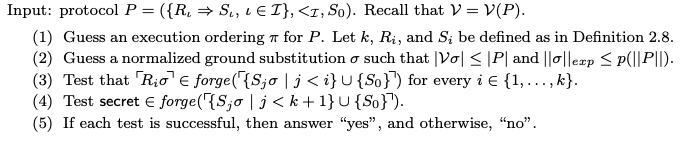
\includegraphics[scale=0.7]{assets/pic01.png}
  \caption{NP‑алгоритм для задачи INSECURE, где p обозначает полином, ограничивающий размер показателей произведений.}
  \label{fig:fig01}
\end{figure}

\begin{enumerate}[label=(\arabic*), leftmargin=0pt, labelwidth=1.5em, labelsep=0.5em, itemindent=0em]
\item Для любого сообщения \(t\) и любого конечного множества сообщений \(E\), если
$t\in\mathrm{forge}(E)\;\Longrightarrow\;\text{тогда существует корректная деривация из }E\text{ с целью }t$.

\item Если $F \;\to_{L_{oc}(t)}\;F,\,t\quad\text{и}\quad F,\,t \;\to_{L_{ad}(t)}\;F,\,t,\,a,$ то существует деривация \(D\) из \(F\) с целью \(a\), при этом 
  \(L_{d}(t)\notin D\).

\item Для любого конечного множества сообщений \(F\) с \(1\in F\), если $F\setminus\{u\}\;\to_{\mathcal{L}_{oc}(u)}\;F$, то есть \(u\) может быть получено из \(F\setminus\{u\}\) за один шаг,   тогда из $F\;\to_{\mathcal{L}_{oc}(u)}\;F,\,t$ следует $\ulcorner t[u\leftarrow1]\urcorner \;\in\;\mathrm{forge}\bigl(\ulcorner F[u\leftarrow1]\urcorner\bigr)$
  для любого сообщения \(t\).
\end{enumerate}

  \section{NP-алоритм принятия решения}

Теперь сформулируем одну из основных теорем этой работы, утверждающую, что задача \textsc{INSECURE} разрешима в классе \textsf{NP} для любого множества оракульных правил, удовлетворяющего двум условиям. Данная общая теорема будет применена в разделе 4 и разделе 7, чтобы показать, что \textsc{INSECURE} остаётся в \textsf{NP} в присутствии злоумышленника, способного выполнять экспоненциацию Диффи–Хеллмана и использовать коммутативное шифрование с открытым ключом, соответственно.

В теореме предъявляются два требования к множеству оракульных правил. Первое: проблема проверки применимости оракульного правила должна решаться эффективно. Второе: множество правил должно допускать полиномиальные атаки на показатели произведений.

\medskip
\textsc{Определение 3.1.} Задача \emph{oracle rule problem} задаётся как
\[
\mathsf{OracleRule}
\;=\;
\{(E,m)\mid E \;\to_{L_o}\; E,\,m\},
\]
где \(E\) — конечное нормализованное множество стандартных сообщений, а \(m\) — стандартное сообщение; оба подаются в виде DAG.

Говорят, что множество оракульных правил \(\mathcal{L}_o\) \emph{допускает полиномиальные атаки на показатели произведений}, если для любого протокола \(P\) и любой минимальной атаки \((\pi,\sigma)\) на этот протокол существует подстановка \(\sigma'\) такая, что $\sigma'\approx\sigma$
(напомним, это означает совпадение \(\sigma'\) и \(\sigma\) с точностью до показателей произведений), пара \((\pi,\ulcorner\sigma'\urcorner)\) является атакой на \(P\), и  $\|\sigma'\|_{\mathrm{exp}}$
полиномиально ограничена по \(\|P\|\). Заметим, что по лемме 2.4 из этого также следует полиномиальная ограниченность \(\|\ulcorner\sigma'\urcorner\|\) по \(\|P\|\).

\medskip
\textsc{Теорема 3.1.} Пусть \(L_o\) — множество оракульных правил. Если
\begin{itemize}
  \item $\mathsf{OracleRule}\in\mathsf{P}\textsf{TIME}$ и
  \item $L_o\text{ допускает полиномиальные атаки на показатели произведений},$
\end{itemize}
то задача \textsc{INSECURE} лежит в классе \(\mathsf{NP}\).

Теорема доказывается следующим образом. Сначала показывается, что недетерминированный алгоритм из рисунка 1 является недетерминированным полиномиальным алгоритмом и корректно решает задачу \textsc{INSECURE}. Полином \(p\), ограничивающий размер показателей произведений, существует в силу того, что \(L_o\) допускает полиномиальные атаки на показатели произведений. Структура алгоритма такова: на шагах 1 и 2 недетерминированно выбирается «маленькая» атака \((\pi,\sigma)\) на протокол \(P\), а на шагах 3 и 4 проверяется, действительно ли \((\pi,\sigma)\) является атакой на \(P\).

Очевидно, что алгоритм из рисунка 1 корректен. Основная же сложность состоит в том, чтобы доказать полиномиальность его работы. Это делается с помощью результатов из разделов 3.1, 3.2 и 3.3. В дальнейшем мы сначала изложим эти результаты, а затем на их основе докажем полноту алгоритма и оценим его временную сложность.

В разделе 3.1 (см. теорему 3.2) показывается, что следующая задача, далее называемая \emph{задачей вывода (derivation problem)}, решается за полиномиальное время от \(\lVert E,t\rVert\), при условии, что \(\mathsf{OracleRule}\) разрешима в детерминированном полиномиальном времени:
\[
\mathsf{Derive} \;:=\; \bigl\{(E,t)\mid t\in\mathrm{forge}(E)\bigr\},
\]
где \(E\) — конечное множество стандартных сообщений, а \(t\) — стандартное сообщение, заданные в виде DAG.

В разделе 3.2 (см. утверждение 3.14) доказывается, что подстановки минимальных атак строятся из подтермов термов, встречающихся в описании протокола.

На основе предложения 3.14 в разделе 3.3 оценивается число подтермов в подстановках минимальных атак и выводится неравенство \(\lvert\sigma\rvert \le \lvert P\rvert\) (следствие 3.16).

Учитывая эти результаты, можем записать доказательство теоремы 3.1.

\medskip
\noindent\textbf{Доказательство теоремы 3.1.}  
Покажем, что алгоритм из рисунка 1 работает в недетерминированное полиномиальное время и является корректным и полным. Корректность уже была отмечена.

Для доказательства полноты нужно убедиться, что если существует атака \((\pi,\sigma)\) на протокол \(P\), то найдётся атака с подстановкой \(\sigma'\), размер которой ограничен так, как это требуется в шаге 2 алгоритма из рисунка 1. Это немедленно следует из следствия 3.16 и предположения, что \(L_o\) допускает полиномиальные атаки на показатели произведений.

Остаётся показать, что наш алгоритм выполняется в недетерминированное полиномиальное время по величине \(\lVert P\rVert\). Для шагов 1 и 2 это очевидно. Чтобы убедиться в полиномиальности шагов 3 и 4, воспользуемся теоремой 3.2. Пусть $E \;=\;\{\ulcorner S_j\sigma\urcorner \mid j<i\}\;\cup\;\{\ulcorner S_0\urcorner\}$
для некоторого \(i\in\{1,\dots,k\}\), а \(t\) обозначает либо \(\ulcorner S_0\urcorner\), либо \(\mathit{secret}\). По теореме 3.2 проверка $t \;\in\;\mathit{forge}(E)$
может быть выполнена за детерминированное полиномиальное время от \(\lVert E,t\rVert\). По следствию 3.16 имеем
$|E,t| \;\le\;|P|$. Поскольку \(\|\sigma\|_{\mathrm{exp}}\) полиномиально ограничено по \(\lVert P\rVert\), то то же верно и для
$\Bigl\|\{\ulcorner S_j\sigma\urcorner\mid j<i\}\cup\{\ulcorner S_0\urcorner\}\cup\{R_i\sigma\}\Bigr\|_{\mathrm{exp}}$.
По лемме 2.4 из этого следует, что \(\lVert E,t\rVert_{\mathrm{exp}}\) полиномиально ограничено по \(\lVert P\rVert\). Следовательно, шаги 3 и 4 могут быть выполнены за детерминированное полиномиальное время по \(\lVert P\rVert\).  
\(\Box\)

\subsection{Решение задачи вывода}

Покажем, что задачу вывода (derivation problem) можно решить за полиномиальное время, при условии, что задача \\textsf{OracleRule} разрешима в детерминированном полиномиальном времени.

\medskip
\noindent\textbf{Теорема 3.2.} Задача
\[
\mathsf{Derive} \;:=\; \{(E,t)\mid t\in\mathrm{forge}(E)\}
\]
разрешима в классе \textsf{P}\textsf{TIME}, при условии, что \(\mathsf{OracleRule}\in\textsf{P}\textsf{TIME}\).

\begin{proof}
Пусть $d_{t}(E)=\{\,t'\in S(E,t)\mid E\;\to_{L_o}\;E,t'\}$
— множество сообщений $t'$, выводимых из $E$ за один шаг. Поскольку число таких $t'$ линейно по $\|E,t\|$, а проверка шага 
$E\;\to_{L_o}\;E,t'$
выполняется за детерминированное полиномиальное время от $\|E,t\|$, нетрудно убедиться, что $d_{t}(E)$ вычисляется за полиномиальное время от $\|E,t\|$. 
Теперь предположим, что $t\in\mathrm{forge}(E)$. По определению 2.11 существует корректная деривация
$D:\quad E \;\to_{L_{1}}\;E, t_{1} \;\to\;\dots\; \to_{L_{r}}\;E, t_1, \dots, t_r$,
где $t_{r}=t$. В частности, $t_{i}\in S(E,t)$ при $i=1,\dots,r$, и все $t_{i}$ попарно различны, поэтому $r\le|E,t|$. Введём рекурсию
$d_{t}^{0}(E):=E, \qquad d_{t}^{i+1}(E):=d_{t}\bigl(d_{t}^{i}(E)\bigr)$.
Очевидно, что 
$t\in d_{t}^{r}(E) \quad\Longleftrightarrow\quad t\in\mathrm{forge}(E)$.
Поскольку каждый шаг вычисления $d_{t}^{i}(E)$ занимает полиномиальное время от $\|E,t\|$, вытекает, что проверка $t\in\mathrm{forge}(E)$ также выполняется за детерминированное полиномиальное время.  
\end{proof}

\subsection{Характеризация подтермов минимальных атак}

Далее мы покажем, что подстановки минимальных атак могут быть сконструированы путём «связывания» подтермов, которые изначально встречаются в спецификации задачи (см. Утверждение 3.14). Для доказательства этого утверждения сначала установим некоторые свойства замен (Леммы 3.4–3.6), затем свойства подстановок в минимальных атаках (Леммы 3.7–3.9) и, наконец, свойства дериваций (Леммы 3.10–3.13).

В дальнейшем мы всегда предполагаем, что \(L_{o}\) — множество оракульных правил. Если \(t\in\mathrm{forge}(E)\), то обозначим через \(D_{t}(E)\) некоторую корректную деривацию из \(E\) с целью \(t\) (выбранную произвольно). Такая деривация всегда существует в силу определения оракульных правил.

Пусть $P=\bigl(\{\,R_i\Rightarrow S_i\mid i\in\mathcal{I}\},\;\prec_{\mathcal{I}},\;S_0\bigr)$ — протокол, а \((\pi,\sigma)\) — атака на \(P\). Пусть \(k=|\pi|\), а \(R_i\) и \(S_i\) определены согласно Определению 2.8. Напомним, что
$S(P)=S_0\;\cup\;\bigcup_{i\in\mathcal{I}}(R_i\cup S_i), \qquad \mathcal{V}(P)=\mathcal{V}\bigl(S(P)\bigr)$.
Также нам понадобится следующее ключевое понятие.

\textsc{Определение 3.3.} Пусть \(t\) и \(t'\) — два терма, а \(\theta\) — наземная подстановка. Тогда говорят, что \(t\) является \(\theta\)\nobreakdash‑соответствием (или \(\theta\)\nobreakdash‑match) терма \(t'\), что обозначается
\[
t \;\sqsubseteq_{\theta}\; t',
\]
если \(t\) и \(t'\) — стандартные термы и
\[
\ulcorner t\,\theta \urcorner\;=\; t'.
\]

\subsubsection*{3.2.1 Свойства замен}

Следующие леммы устанавливают дистрибутивные свойства функции нормализации, подстановок, оператора экспоненциации и операций замены.

\textsc{Лемма 3.4.} Пусть \(u\) — нормализованный терм, а \(M, M'\) — два произведения, такие что все подтермы из \(\mathcal{F}(M)\cup \mathcal{F}(M')\) нормализованы. Пусть \(s\) — стандартный нормализованный терм, а \(\delta=[s\leftarrow 1]\) — замена. Тогда выполняются равенства:

(1)\quad 
\(\ulcorner (M\cdot M') \delta \urcorner
   =\ulcorner\ulcorner M\cdot M'\urcorner\delta\urcorner\),
в частности 
\(\ulcorner M\delta\urcorner=\ulcorner\ulcorner M\urcorner{\delta}\urcorner\).

(2)\quad 
\(\ulcorner Exp(u,M)\delta\urcorner
   =\ulcorner\ulcorner Exp(u,M)\urcorner\delta\urcorner\),
если \(s\neq\ulcorner Exp(u,M)\urcorner\),
и, в случае если \(s=Exp(\cdot,\cdot)\), также \(s\neq u\).

\begin{proof}
См.~Приложение~A\qedhere
\end{proof}

\medskip
Отметим, что пункт 2 в предыдущей лемме не выполняется без ограничений на $s$.
Следующий пример демонстрирует проблему при
$s=\ulcorner Exp(u,M)\urcorner$:
предположим, что $s=Exp(a,b)$, $u=a$, а
$M=b\!\cdot\!c\!\cdot\!c^{-1}$.
Тогда
$s=\ulcorner Exp(u,M)\delta\urcorner
\neq
\ulcorner\ulcorner Exp(u,M)\urcorner\delta\urcorner=1$.  
Следующий пример иллюстрирует, почему необходимо требование $s\neq u$:
положим $s=u=Exp(a,b)$ и $M=c$.
Тогда
$1=\ulcorner Exp(u,M)\delta\urcorner
\neq
\ulcorner\ulcorner Exp(u,M')\urcorner\delta\urcorner
=Exp(a,b\!\cdot\!c)$.

\textsc{Лемма 3.5.} 
Пусть $\sigma$ — нормализованная замкнутая подстановка,
$E$ — множество нормализованных терминов,
$s$ — нормализованный стандартный неатомарный термин,
а $\delta$ — замена $[s \leftarrow 1]$.
Обозначим $\sigma'=\ulcorner\sigma\delta\urcorner$.
Если не существует стандартного подтермина $t\in E$ такого, что  
$t\sqsubseteq_{\sigma}s$, то $\ulcorner E\sigma'\urcorner = \ulcorner\ulcorner E\sigma\urcorner\delta\urcorner$.

\begin{proof}
  См.\ Приложение~A.
\end{proof}

\medskip

\textsc{Лемма 3.6.} 
Пусть $t',\,t_1,\dots,t_n,\,t,\,u$ — нормализованные стандартные термины,
$z_1,\dots,z_n\in\mathbb Z$, а $\delta$ — замена $[u\leftarrow1]$ такая, что
$u\neq t$ и $t=\ulcorner Exp\bigl(t',\,t_1^{\,z_1}\!\cdots t_n^{\,z_n}\bigr)\urcorner$.
Если $t'=Exp(\,\cdot,\cdot\,)$, то дополнительно предполагаем
$u\neq t'$. Тогда
\[
  \ulcorner t\delta\urcorner
  =\ulcorner Exp\bigl(\ulcorner t'\delta\urcorner,
        \ulcorner t'\delta\urcorner^{z_1}\!\cdots \ulcorner t_n\delta\urcorner^{z_n}\bigr)\urcorner.
\]

\begin{proof}
  См.\ Приложение А.
\end{proof}

\subsubsection*{3.2.2 \,Свойства подстановок минимальных атак}
Следующая лемма позволяет доказать то, что мы далее будем
называть \emph{свойством единственного сопоставления}.

\textsc{Лемма 3.7.}
Пусть $s$ — стандартный термин, $t$ — нормализованный термин,
а $\sigma$ — нормализованная подстановка такая, что
$s\in S(\ulcorner t\sigma\urcorner)$ и
$s\notin S(x\sigma)$ для каждого $x\in\mathcal V(t)$.
Тогда существует стандартный подтермин $t'$ термина $t$,
удовлетворяющий $t'\sqsubseteq_{\sigma}s$.

\textit{Доказательство.}
По лемме 2.4 имеем
\[
  S(\ulcorner t\sigma\urcorner)\;\subseteq\;
  \ulcorner S(t\sigma)\urcorner
  \;\subseteq\;
  \ulcorner S(t)\sigma\;\cup\;\mathcal V(t)\sigma\urcorner.
\]
Так как $\sigma$ находится в нормальной форме, это означает
\[
  S(\ulcorner t\sigma\urcorner)\;\subseteq\;
  \ulcorner S(t)\sigma\urcorner\;\cup\;\mathcal V(t)\sigma.
\]
По предположению $s\in \mathcal S(\ulcorner t\sigma\urcorner)$ и
$s\notin \mathcal S(\mathcal V(t)\sigma)$.
Следовательно, $s\in\ulcorner \mathcal S(t)\sigma\urcorner$,
то есть существует $t'\in \mathcal S(t)$ такое, что
$\ulcorner t'\sigma\urcorner = s$.
\hfill$\square$

Теперь мы докажем \emph{свойство единственного сопоставления}:
если злоумышленник посылает сообщения $m_1,\dots,m_i$,
то существует не более одного способа сопоставить эти сообщения
с $R_1,\dots,R_i$ при каждом $R_j,\;j\in\{1,\dots,i\}$,
определённых выше.

\textsc{Лемма 3.8.} \textit{Пусть дана произвольная последовательность
нормализованных сообщений $m_1,\dots,m_i$.
Существует не более одной нормализованной подстановки $\sigma$ такой, что
\(
  \ulcorner R_j\sigma\urcorner = m_j
\)
для всех $j\in\{1,\dots,i\}$.}

\textit{Доказательство.}
Предположим противное и выберем минимальный
$i\in\{1,\dots,n\}$, для которого существуют две разные
нормализованные подстановки $\sigma$ и $\sigma'$, удовлетворяющие
\(
  \ulcorner R_j\sigma\urcorner=\ulcorner R_j\sigma'\urcorner
\)
для всех $j\in\{1,\dots,i\}$.
Из минимальности $i$ следует, что $\sigma$ и $\sigma'$
совпадают на
\(V_{i-1}=\mathcal V(R_1,\dots,R_{i-1})\)
и различаются на некоторой переменной из
\(\mathcal V(R_i)\setminus V_{i-1}\).
Обозначим через $\sigma_0$ подстановку, равную
$\sigma$ на $V_{i-1}$ и тождественную
на \(\mathcal V(R_i)\setminus V_{i-1}\);
положим \(r=\ulcorner R_i\sigma_0\urcorner\).

По Лемме 2.4, 5 и поскольку
\(R_i\sigma=(R_i\sigma_0)\sigma\) и
\(R_i\sigma'=(R_i\sigma_0)\sigma'\),
получаем
\(
  \ulcorner R_i\sigma\urcorner
  =\ulcorner r\sigma\urcorner
  =\ulcorner r\sigma'\urcorner.
\)
По предположению найдётся переменная
\(x\in\mathcal V(r)\) такая, что \(x\sigma\ne x\sigma'\).
Выберем \(t_x\in \mathcal S(r)\) минимальный
(относительно отношения «подтермин»),
для которого \(x\in\mathcal V(t_x)\) и
\(
  \ulcorner t_x\sigma\urcorner
  =\ulcorner t_x\sigma'\urcorner.
\)
Так как $r$ является возможным кандидатом,
такой термин $t_x$ корректно определён.

Очевидно, $t_x$ не может быть ни переменной, ни константой.
На самом деле легко видеть, что
\(t_x\) обязан иметь вид
\(
  Exp(t_1,t_2^{z_2}\!\cdots t_k^{z_k}).
\)
По Определению 2.6, 3 и так как \(x\in\mathcal V(t_x)\),
для всех \(j\in\{1,\dots,k\}\setminus\{j_0\}\)
термины \(t_j\) являются замкнутыми.
Пусть \(j_0\) — индекс незамкнутого подтермина, т.\,е.\ \(x\in\mathcal V\!\bigl(t_{j_0}\bigr)\).
По минимальности \(t_x\) имеем \(t_{j_0}\sigma\neq t_{j_0}\sigma'\).
Учитывая, что \(t_x\sigma=t_x\sigma'\), рассмотрим возможные случаи:

— $j_0 = 1$: Сначала предположим, что
\(
  \ulcorner t_{j_0}\sigma \urcorner = Exp(b,M)
\)
и
\(
  \ulcorner t_{j_0}\sigma' \urcorner = \operatorname{Exp}(b',M').
\)
Так как \(\ulcorner t_x\sigma \urcorner = \ulcorner t_x\sigma' \urcorner\), имеем
\(b=b'\) и
\(
  \ulcorner M\!\cdot\!\prod_{i=2}^{k} t_i^{z_i} \urcorner
  =
  \ulcorner M'\!\cdot\!\prod_{i=2}^{k} t_i^{z_i} \urcorner.
\)
Отсюда \(M=M'\) и, следовательно,
\(\ulcorner t_{j_0}\sigma \urcorner = \ulcorner t_{j_0}\sigma'\urcorner\),
что противоречит предположению. Если оба термина \(\ulcorner t_{j_0}\sigma \urcorner\) и \(\ulcorner t_{j_0}\sigma' \urcorner\)
не имеют вида \(\operatorname{Exp}(\,\cdot,\cdot\,)\),
то из равенства \(\ulcorner t_x\sigma \urcorner = \ulcorner t_x\sigma' \urcorner\)
также немедленно следует
\(\ulcorner t_{j_0}\sigma \urcorner = \ulcorner t_{j_0}\sigma' \urcorner \).
Если же
\(\ulcorner t_{j_0}\sigma \urcorner = \operatorname{Exp}(b,M)\),
а \(\ulcorner t_{j_0}\sigma' \urcorner\) не имеет вида
\(\operatorname{Exp}(\,\cdot,\cdot\,)\),
то равенство \(\ulcorner t_x\sigma \urcorner = \ulcorner t_x\sigma' \urcorner \)
влечёт
\(
  \ulcorner M\!\cdot\!\prod_{i=2}^{k} t_i^{z_i} \urcorner
  =
  \ulcorner \prod_{i=2}^{k} t_i^{z_i}\urcorner,
\)
а значит \(M=1\), что противоречит тому, что
\(t_{j_0}\sigma\) нормализован.
Следовательно, случай \(j_0 = 1\) невозможен.

— $j_0>1$:  
Сначала предположим, что \(t_1 = Exp(b,M)\).
Из равенства \(\ulcorner t_x\sigma\urcorner = \ulcorner t_x\sigma'\urcorner\) получаем
\[
  \ulcorner M \!\cdot\!
  \ulcorner t_{j_0}^{z_{j_0}}\sigma \urcorner\!
  \cdot
  \prod_{j\in\{2,\dots,k\}\setminus\{j_0\}}
     \bigl(t_j\bigr)^{z_j}\urcorner
  \;=\;
  \ulcorner M\;\cdot\;
  \ulcorner t_{j_0}^{\,z_{j_0}}\sigma'\urcorner\;
  \cdot\!
  \prod_{j\in\{2,\dots,k\}\setminus\{j_0\}} t_j^{\,z_j}\urcorner
\]
Следует
\(
  \bigl(t_{j_0}\sigma\bigr)^{z_{j_0}}
  =
  \bigl(t_{j_0}\sigma'\bigr)^{z_{j_0}},
\)
что противоречит выбору \(t_{j_0}\).
Случай, когда \(t_x\sigma\) не имеет вида
\(\operatorname{Exp}(\,\cdot,\cdot\,)\),
разбирается ещё проще. \qed

Используя предыдущую лемму, покажем, что любой подтермин подстановки,
соответствующей минимальной атаке,
либо принадлежит спецификации протокола,
либо является подтермином нормализованного сообщения,
передаваемого в ходе атаки.

\textsc{Лемма 3.9.}
Пусть \((\pi,\sigma)\) — атака на \(P\) с нормализованной подстановкой
\(\sigma\),
\(x\in\mathcal V(R_i)\) для некоторого
\(i\in\{1,\dots,k\}\),
а \(s\in \mathcal S\!\bigl(\sigma(x)\bigr)\) — стандартный термин.
Тогда существует \(j\le i\) такое, что
\(
  s\in \mathcal S\!\bigl(\ulcorner R_j\sigma\urcorner\bigr)
\)
или существует \(t\in S(P)\) со свойством \(t\sqsubseteq_{\sigma}s\).

\textit{Доказательство.}
Предположим, что не существует \(t\in S(P)\) такого, что
\(t\sqsubseteq_{\sigma}s\),
и при этом
\(s\notin S\!\bigl(\ulcorner R_j\sigma\urcorner\bigr)\)
для всех \(j\le i\).
Отсюда \(s\) не является атомом.
Положим
\(V_j=\mathcal V(R_j)\cup\mathcal V(S_j)\)
и выберем минимальный \(j\), для которого
\(s\in S\!\bigl(V_j\sigma\bigr)\).
По Определению 2.6, 2 имеем
\(s\in S\!\bigl(\mathcal V(R_j)\sigma\bigr)\).
Обозначим
\(
  \sigma'=\ulcorner \sigma[s\!\leftarrow\!1]\urcorner.
\)

По минимальности \(j\) для всех \(l<j\) выполняется
\(R_l\sigma'=R_l\sigma\),
а значит
\(
  \ulcorner R_l\sigma'\urcorner
  =
  \ulcorner R_l\sigma\urcorner.
\)
Поскольку
\(s\notin S\!\bigl(\ulcorner R_j\sigma\urcorner\bigr)\),
получаем
\(
  \ulcorner R_j\sigma'\urcorner[s\!\leftarrow\!1]
  =
  \ulcorner R_j\sigma\urcorner.
\)
По Лемме 3.5 отсюда следует
\(
  \ulcorner R_j\sigma\urcorner
  =
  \ulcorner R_j\sigma'\urcorner.
\)
Заметим, что \(\sigma\) и \(\sigma'\) различаются
хотя бы по одной переменной из
\(\mathcal V(R_1,\dots,R_j)\),
что противоречит Лемме 3.8.\hfill$\square$

\subsubsection*{3.2.3 \,Свойства выводов}
Ниже приводятся несколько полезных свойств выводов, 
позволяющих без труда заменять термины внутри вывода.
Начнём с простого наблюдения, непосредственно вытекающего
из определения правил декомпозиции и композиции.

\textsc{Лемма 3.10.}
Пусть $E$ — нормализованное конечное множество сообщений,
$t$ — сообщение,
а $L$ — $t$-правило, для которого выполнен один шаг вывода
\(
  E \rightarrow_{L} E,\,t,
\)
и при этом $\mathcal S(E,t)\ne \mathcal S(E)$.
Тогда
\(
  \mathcal S(E,t)=\mathcal S(E)\cup\{t\},
\qquad
  \text{и }L\text{ является правилом композиции.}
\)

Следующая лемма утверждает, что если
$t'$ — подтермин термина $t$,
термин $t$ выводится из множества $E$,
но при этом $t'$ не является подтермином ни одного элемента $E$,
то $t'$ также выводится из $E$, причём
последним шагом такого вывода служит правило композиции.

\textsc{Лемма 3.11.}
Предположим, что
$t'\in \mathcal S(t)\setminus \mathcal S(E)$
и
$t\in forge(E)$.
Тогда
\(
  t'\in forge(E),
\)
и существует вывод из $E$ с целью $t'$,
завершающийся правилом композиции.

\begin{proof}
Пусть
\(D=E_0 \rightarrow_{\,L_1\,} E_1 \;\cdots\; \rightarrow_{\,L_n\,} E_n\)
— вывод термина \(t\), причём \(E_0 = E\).
Так как \(t'\) является подтермином элементов \(E_n\),
существует минимальный \(i>0\) такой, что
\(t' \in \mathcal S(E_i)\).
По минимальности \(i\) имеем
\(t'\in \mathcal S(E_i)\setminus \mathcal S(E_{i-1})\).
Применяя Лемму 3.10, заключаем, что
\(D=E_0 \rightarrow_{\,L_1\,} E_1 \;\cdots\; \rightarrow_{\,L_i\,} E_i\)
— это вывод с целью \(t'\).
\end{proof}

\noindent лемма будет использована в доказательстве Леммы 3.13.
Она позволяет строить специальные выводы, в которых заданный термин
никогда не декомпозируется. Это окажется критически важным,
когда потребуется заменить составные термины атомами в ряде выводов.

\textsc{Лемма 3.12.}
Пусть $t\in forge(E)$ и $\gamma\in forge(E)$.
Предположим, что имеется вывод $D_{\gamma}$ из $E$,
последним шагом которого является применение правила из $\mathcal L_{c}$.
Тогда существует вывод $D'$ из $E$ с целью $t$, удовлетворяющий
\(
  L_{d}(\gamma)\notin D'.
\)

\begin{proof} См.\ Приложение А.\end{proof}

\medskip

Теперь мы можем сформулировать лемму, позволяющую
заменять определённые подтермины, возникающие в подстановке атаки,
на более короткие.
Из предположений текущей леммы следует, что
$s$ выводим из $E$ так, что последним правилом является правило композиции.
Это даёт возможность заменить $s$ на более короткий термин,
поскольку при выводе $t$ декомпозиция $s$ уже не потребуется.

\textsc{Лемма 3.13.}
Пусть $E$ и $F$ — два множества нормализованных сообщений, причём
$1\in E\cup F$.
Пусть
$t\in forge(E,F)$ и
$s\in forge(E)$ — неатомарный термин, причём $s\notin \mathcal S(E)$.
Обозначим через $\delta$ подстановку $[\,s\!\leftarrow\!1\,]$.
Тогда
\(
  \ulcorner t\delta\urcorner\;\in\;
   forge\!\bigl(\,\ulcorner E\delta,\,F\delta\urcorner\bigr).
\)

\begin{proof}
По лемме 3.11 существует корректный вывод
$D_s$ из $E$ с целью $s$, в котором последний шаг — правило композиции.
По лемме 3.12 имеется вывод
$D_t$ из $E,F$ с целью $t$, такой, что $L_d(s)\notin D_t$.
Запишем
\(
  D_t:\quad
  E,F \rightarrow_{L_1} E,F,t_1
       \rightarrow_{L_2} E,F,t_2
       \;\cdots\;
       \rightarrow_{L_n} E,F,t_1,\dots,t_n .
\)

Покажем по индукции по $i\;(0\le i\le n)$, что
\[
  \ulcorner t_i\delta\urcorner\;\in\;
   forge\!\bigl(\,\ulcorner E\delta,\,F\delta\urcorner\bigr).
\]

\noindent\emph{База.}
Если $t_0\in E\cup F$, то
\(
  \ulcorner t_0\delta\urcorner\in
  \ulcorner E\delta\cup F\delta\urcorner
  \subseteq
  forge\!\bigl(\,\ulcorner E\delta,\,F\delta\urcorner\bigr).
\)

\emph{Индукционный шаг.}
Пусть утверждение доказано для всех $j<i$; рассмотрим правило $L_i$.

\begin{itemize}
  \item[--$L_i=L_c(\langle a,b\rangle)$:]
        либо $t_i=s$ и тогда
        $t_i\delta=1\in forge(E\delta,F\delta)$,
        либо
        $t_i\delta=\langle a\delta,b\delta\rangle$.
        По предположению индукции
        $\{a\delta,b\delta\}\subseteq
          forge\!\bigl(\,\ulcorner E\delta,\,F\delta\urcorner\bigr)$,
        откуда
        $t_i\delta\in
         forge\!\bigl(\,\ulcorner E\delta,\,F\delta\urcorner\bigr)$.
        Аналогично разбираются случаи $\{a\}_b^{\,s}$ и $\{a\}_K^{\,p}$.

  \item[--$L_i=L_{p1}(\langle t_i,a\rangle)$:]
        здесь $s\neq\langle t_i,a\rangle$,
        так как $L_i\notin L_d(s)$.
        Получаем
        $\langle t_i,a\rangle\delta=\langle t_i\delta,a\delta\rangle$.
        По индукционной гипотезе
        $\langle t_i,a\rangle\delta\in
         forge(E\delta,F\delta)$,
        следовательно
        $t_i\delta\in forge(E\delta,F\delta)$.
        Точно так же обрабатываются правила
        $L_{p2},L_{sd}$ и $L_{ad}$.

  \item[--$L_i\in L_o$:]
        воспользуемся Определением 2.11, 3.
        Пусть $E'$ — множество сообщений, полученное в $D_s$
        непосредственно перед применением последнего шага.
        Тогда
        $E'\setminus\{s\}\rightarrow_{\mathcal L_c(s)}E',s$,
        а также
        \[
          E,F,t_1,\dots,t_{i-1}\rightarrow_{L_i}
          E,F,t_1,\dots,t_i .
        \]
        В частности,
        $E',E,F,t_1,\dots,t_{i-1}\rightarrow_{L_i}E',E,F,t_1,\dots,t_{i-1},t_{i}$,
        откуда по Определению 2.11, 3
        \[
          \ulcorner t_i\delta\urcorner\in
          forge\!\bigl(
            \ulcorner E'\delta,\,
            E\delta,\,F\delta,\,
            t_1\delta,\dots,t_{i-1}\delta\urcorner
          \bigr).
        \]
        Заметим, что $E'\delta=E'$, $E\delta=E$,
        а все сообщения из $E'$ выводимы из $E$.
        Индукционное предположение даёт
        $\ulcorner t_1\delta \urcorner,\dots,\ulcorner t_{i-1}\delta \urcorner\in
         forge\!\bigl(\,\ulcorner E\delta,\,F\delta\urcorner\bigr)$,
        поэтому
        \(
          forge\!\bigl(
            \ulcorner E'\delta,\,
            E\delta,\,F\delta,\,
            t_1\delta,\dots,t_{i-1}\delta\urcorner
          \bigr)
          \subseteq
          forge\!\bigl(\,\ulcorner E\delta,\,F\delta\urcorner\bigr),
        \)
        и поэтому
        \(
          t_i\delta\in
           forge\!\bigl(\,\ulcorner E\delta,\,F\delta\urcorner\bigr).
        \)
\end{itemize}

Для $i=n$ получаем
\(
  t\delta\in forge(E\delta,F\delta),
\)
что и требовалось.
\end{proof}

\subsubsection*{3.2.4 \,Свойства минимальных атак}

Теперь мы готовы перейти к доказательству Предложения 3.14, которое утверждает, что
подстановки минимальных атак всегда можно построить,
связывая подтермины, изначально присутствующие в протоколе~$P$.
Это ключевой шаг, позволяющий ограничить число подтерминов
в минимальных атаках (см.\ Теорему 3.15).

\textsc{Предложение 3.14.}
Пусть $(\pi,\sigma)$ — минимальная атака на протокол $P$.
Тогда для любого
\(s\in S(\mathcal V\sigma)\)
существует
\(t\in \mathcal S(P)\) такое, что \(t\sqsubseteq_{\sigma}s\).

\begin{proof}
Положим $(\pi,\sigma)$ и $s$ как выше.
Предположим обратное\;(*)\,: \emph{для каждого $t$ из условия
$t\sqsubseteq_{\sigma}s$ следует $t\notin \mathcal S(P)$}.
Доведём это допущение до противоречия.

Так как $\mathcal A\subseteq \mathcal S(P)$, получаем $s\notin \mathcal A$.
По лемме 3.9 и (*)
существует $j$ такое, что
\(s\in \mathcal S\!\bigl(\ulcorner R_j\sigma\urcorner\bigr)\).
Выберем минимальный среди возможных $j$ и
рассмотрим $N=j$.
Если
\(s\in \mathcal S\!\bigl(\ulcorner S_i\sigma\urcorner\bigr)\)
для некоторого $i$, то (*)
и лемма 3.7 дают нам переменную
\(x\in\mathcal V(S_i)\) с
\(s\in S(x\sigma)\).
По определению 2.6, (2)
существуют $R_{i'},i'\le i$ такие, что
\(x\in\mathcal V(R_{k})\).
Следовательно, леммы 3.9 и (*) вновь
дают индекс $j\le i$ с
\(s\in S\!\bigl(\ulcorner R_j\sigma\urcorner\bigr)\).
Заметим, что
\(s\notin \mathcal S(S_0)\), иначе
\(s\in \mathcal S(P)\), и (*)
бы не выполнялось.
Минимальность $N$ гарантирует $i\ge N$.
Положим
\(E_j=\ulcorner S_0\sigma,\dots,S_{j-1}\sigma \urcorner\).
Итак, $s$ — неатомарный термин,
не являющийся подтермином $E_N$,
но являющийся подтермином
\(\ulcorner R_N\sigma\urcorner\);
по лемме 3.11 тогда
\(s\in forge(E_N)\).

Обозначим $\delta=[\,s\!\leftarrow\!1\,]$.
Поскольку $(\pi,\sigma)$ — атака,
для всех $1\le j\le k+1$
(где $R_{k+1}=\textit{secret}$) выполняется
\[
  \ulcorner R_j\sigma\urcorner \;\in\;
   forge(E_j).
\]

Рассмотрим два случая.

\medskip
\noindent— \textbf{$j<N$.}
Минимальность $N$ означает, что $s$ не является подтермином
ни \(\ulcorner R_j\sigma\urcorner\), ни $E_j$.
Тогда из
\(\ulcorner R_j\sigma\urcorner\in forge(E_j)\)
получаем
\(
  \ulcorner\ulcorner R_j\sigma\urcorner\delta\urcorner
  \in
  forge\!\bigl(\ulcorner E_j\delta\urcorner\bigr)
  =forge(E_j\delta).
\)

\medskip
\noindent— \textbf{$j\ge N$.}
Полагая
\(t=\ulcorner R_j\sigma\urcorner,\;E=E_N,\;F=E_j\),
применяем лемму 3.13 и
получаем
\(
  \ulcorner\ulcorner R_j\sigma\urcorner\delta\urcorner
  \in
   forge\!\bigl(\ulcorner E_j\delta\urcorner\bigr).
\)

\noindent
Таким образом,
\(\ulcorner\ulcorner R_j\sigma\urcorner\delta\urcorner\in
  forge(\ulcorner E_j\delta\urcorner)\)
в обоих случаях.
Теперь из (*) и леммы 3.5
для всех $j$ выводим
\[
  \ulcorner R_j\sigma\urcorner
  \in
   forge
  \bigl(
    \ulcorner S_0\sigma',\dots,S_{j-1}\sigma'\urcorner
  \bigr),
  \qquad
  \text{где }\sigma'=\ulcorner\sigma\delta\urcorner.
\]
Следовательно, $(\pi,\sigma')$ также является атакой.
(Условия применения леммы 3.5 выполнены.)
Но $\sigma'$ получена из $\sigma$ заменой $s$ на термин $1$,
то есть
\(|\sigma'|<|\sigma|\),
что противоречит минимальности атаки $(\pi,\sigma)$.
\end{proof}

\subsection{Ограничение числа подтерминов минимальных атак}

Опираясь на Предложение 3.14, получаем:

\textsc{Теорема 3.15.}
Для каждой минимальной атаки $(\pi,\sigma)$ на протокол $P$ выполнено
\[
  \mathcal S\!\bigl(\,\ulcorner \mathcal S(P)\sigma\urcorner\bigr)\;=\;
  \ulcorner \mathcal S(P)\sigma\urcorner.
\]

\textit{Доказательство.}
Включение
\(
  \ulcorner \mathcal S(P)\sigma\urcorner
  \subseteq
  S\!\bigl(\,\ulcorner \mathcal S(P)\sigma\urcorner\bigr)
\)
очевидно.
Обратное включение является прямым следствием
Предложения 3.14, из которого получаем
\[
  \mathcal S(\mathcal V\sigma)
  \subseteq
  \ulcorner \mathcal S(P)\sigma\urcorner.
\]
По лемме 2.4 имеем
\(
  S\!\bigl(\,\ulcorner \mathcal S(P)\sigma\urcorner\bigr)
    \subseteq
  \ulcorner \mathcal S\bigl(\mathcal S(P)\sigma\bigr)\urcorner,
  \qquad
  \mathcal S\bigl(\mathcal S(P)\sigma\bigr)
    \subseteq
  \mathcal S(P)\sigma\;\cup\; \mathcal S(\mathcal V\sigma).
\)
Следовательно,
\(
  \mathcal S\!\bigl(\,\ulcorner \mathcal S(P)\sigma\urcorner\bigr)
    \subseteq
  \ulcorner \mathcal S(P)\sigma\urcorner
  \;\cup\;
  \mathcal S(\mathcal V\sigma),
\)
и, учитывая предыдущее включение,
получаем
\(
  S\!\bigl(\,\ulcorner S(P)\sigma\urcorner\bigr)
    \subseteq
  \ulcorner S(P)\sigma\urcorner.
\)
Тем самым равенство доказано.\hfill$\square$

Из Теоремы 3.15 немедленно следует:

\textsc{Следствие 3.16.}
Для каждой минимальной атаки $(\pi,\sigma)$ на протокол $P$
и любого множества $E\subseteq \mathcal S(P)$ выполняется
\(
  \bigl|\,\ulcorner E\sigma\urcorner\bigr|\;\le\;|P|.
\)
В частности,
\(
  |\,\mathcal V(P)\sigma|\;\le\;|P|.
\)

\begin{proof}
Во-первых, мощность множества
\(\mathcal S\!\bigl(\,\ulcorner \mathcal S(P)\sigma\urcorner\bigr)\)
не превышает $|P|$.
Во-вторых,
\(
  \ulcorner E\sigma\urcorner
  \subseteq
  \mathcal S\!\bigl(\,\ulcorner \mathcal S(P)\sigma\urcorner\bigr),
\)
откуда сразу следует требуемое
\(
  \bigl|\,\ulcorner E\sigma\urcorner\bigr|\le|P|.
\)
Подставляя $E=\mathcal V(P)$, получаем
\(
  |\,\mathcal V(P)\sigma|\le|P|.
\)
Заметим, что $\sigma$ нормализована, поэтому
\(
  \sigma(x)=\ulcorner\sigma(x)\urcorner
\)
для любой переменной $x$.
\end{proof}

  \section{Расширение модели нарушителя Долева–Яо за счёт экспоненцирования Диффи–Хеллмана}

Мы расширяем нарушителя Долева–Яо, определённого правилами
\(L_c \cup L_d\) (см.~п.~2.2), добавляя набор правил \(L_\sigma\) —
\emph{DH-правила}, позволяющих нарушителю выполнять
экспоненцирование Диффи–Хеллмана.
Расширенный нарушитель будем называть \emph{DH-нарушителем}.
Наша цель — показать, что для DH-нарушителя задача вывода решается за детерминированное полиномиальное
время, а задача небезопасности решается за недетерминированное полиномиальное время.
Для этого проверим, что выполняются предпосылки
Теоремы 3.2 и Теоремы 3.1.
Напомним, Теорема 3.2 требует:
\begin{enumerate}
  \item \(L_\sigma\) является множеством оракульных правил и
  \item \textsc{OracleRule} решается за полиномиальное время;
\end{enumerate}
дополнительно Теорема 3.1 требует:
\begin{enumerate}
  \item \(L_\sigma\) допускает полиномиальные «произведение-показатель»-атаки.
\end{enumerate}

В разделах 4.1 и 4.2 мы докажем пункт а),
а в разделе 4.3 — пункт б).
Используя Теорему 3.2, придём к выводу,
что для DH-нарушителя задача вывода
решается за полиномиальное время
(см.~Следствие 4.9).

В разделе 5 мы докажем пункт iii);
совместно с Теоремой 3.1 это даст,
что для DH-нарушителя задача небезопасности
решается за недетерминированное полиномиальное время
(см.~Теорему 5.23).

\medskip
Сначала зададим DH-правила \(L_\sigma\).

\begin{definition}[4.1]
Положим \(L_\sigma = L_{\sigma_c}\cup L_{\sigma_d}\), где
\(L_\sigma\) состоит из всех правил вида
\[
  t,\,t_1,\dots,t_n
  \;\longrightarrow\;
  \ulcorner Exp\!\bigl(t,t_1^{\,z_1}\!\cdots t_n^{\,z_n}\bigr)\urcorner
  \;=:\;u,
\]
где \(n\ge1\), \(z_i\in\mathbb Z\setminus\{0\}\),
\(1\le i\le n\), а \(t,t_1,\dots,t_n\) — нормализованные
стандартные сообщения.  
Если \(u\) имеет вид \(Exp(\cdot,\cdot)\),
то правило входит в
\(L_{\sigma_c}(u)\) (множество \emph{композиционных} DH-правил);
иначе — в \(L_{oc}(u)\) (множество
\emph{декомпозиционных} DH-правил).
Нарушителя, использующего \(L_0\) как оракульные правила,
мы называем \emph{DH-нарушителем}.  
Термин \(t\) в правиле называют \emph{головой} правила, а
\(z_1,\dots,z_n\) — \emph{показателями произведения}.
Будем считать без ограничения общности, что
голова декомпозиционного DH-правила имеет форму \(Exp(\cdot,\cdot)\)
(иначе \(t=u\));
также полагаем \(t_i\neq t_j\) при \(i\neq j\) и \(z_i\neq0\) для всех \(i\).
\end{definition}

\medskip
Так как сообщения в правой части DH-правила нормализованы,
легко получить следующее.

\textsc{Лемма 4.2.}
Правила из \(L_{oc}\) являются композиционными,
а правила из \(L_{od}\) — декомпозиционными правилами угадывания.

\subsection{Диффи–Хеллман правила допускают корректные выводы}

Покажем, что \(L_o\) допускает корректные выводы (лемма 4.5).  
Иными словами, \(L_o\) удовлетворяет первому из требований к «oracle-rules»
(см. определение 2.11).  
Доказательство опирается на две вспомогательные леммы, приведённые ниже.

Первая лемма позволяет ограничиться такими выводами, в которых
правила из \(L_o\) применяются только к тем сообщениям,  
которые были либо созданы правилами Долева–Яо\,(DH),  
либо присутствовали в исходном множестве сообщений.

\textsc{Лемма 4.3.}
Пусть \(E\) — конечное множество нормализованных стандартных сообщений,
\(t\) — стандартное сообщение такое, что \(t\) выводится из \(E\) (относительно \(L\)).
Пусть \(D\) — вывод из \(E\) с целью \(t\).
Тогда существует вывод \(D'\) из \(E\) с той же целью \(t\), удовлетворяющий:

\begin{enumerate}
  \item \(D'\) имеет ту же длину, что и \(D\);
  \item для любого DH-правила \(L\in D'\cap L_{o}\) с головным термом \(t'\)
        выполнено: \(t'\in E\) \;или\;  
        существует \(t'\)-правило \(L'\in D'\cap(L_{d}\cup L_{c})\).
        Более того, если \(L\) — \emph{декомпозиционное} DH-правило,
        то \(t'\in E\) \;или\;
        существует \(t'\)-правило \(L'\in D'\cap L_{d}\).
\end{enumerate}

\begin{proof} См. Приложение Б.\end{proof}

Следующая лемма даёт критерий, позволяющий проверить,
корректен ли вывод.

\textsc{Лемма 4.4.}
Пусть
\(D = E_0 \rightarrow_{\,L_1\,} \dots
      E_{n-1} \rightarrow_{\,L_n\,} E_n\)
— вывод с целью \(g\).

\begin{enumerate}
\item
  Предположим, что для каждого шага
  \(E_{j-1} \rightarrow{\,L_j\,} E_j\) вывода \(D\)
  с \(L_j \in \mathcal L_{d}(t)\)
  существует \(t'\in E_{j-1}\) такое, что
  \(t \sqsubseteq t'\) и
  \(t'\in E_0\) \;или\;
  \(\exists\,i<j: L_i\in \mathcal L_{d}(t')\).
  Тогда из \(L\in D\cap \mathcal L_{d}(t)\)
  (для некоторого \(\mathcal L,t\)) следует
  \(t\in \mathcal S(E_0)\).

\item
  Предположим, что для каждого \(i<n\) и \(t\) с
  \(L_i\in \mathcal L_{c}(t)\)
  найдётся \(j>i\) такое, что
  \(L_j\) является \(t'\)-правилом
  и \(t\in \mathcal S\bigl(\{t'\}\cup E_0\bigr)\).
  Тогда из \(L\in D\cap \mathcal L_{c}(t)\)
  (для некоторого \(L,t\)) следует
  \(t\in \mathcal S(E_0,g)\).
\end{enumerate}

При выполнении обеих предпосылок (а) и (б)
вывод \(D\) является корректным 
выводом с целью \(g\).

\begin{proof} См.\ Приложение Б.\end{proof}

Теперь мы можем показать, что правила \(L_{o}\) допускают
корректные выводы.

\textsc{Лемма 4.5.}
Пусть \(E\) — конечное нормализованное множество стандартных сообщений,
а \(g\) — нормализованное стандартное сообщение.
Если \(g\in forge(E)\),
то существует корректный вывод из \(E\) с целью \(g\).

\begin{proof}
Положим \(E_{0}=E\) и
\(
  D\;=\;
  E_{0}\rightarrow_{\,L_{1}\,}
  \dots
  \rightarrow_{\,L_{n}\,}E_{n}
\)
— вывод цели \(g\) минимальной длины.
Будем считать, что \(D\) удовлетворяет свойствам,
сформулированным в лемме 4.3, пункт 2.

Покажем, что \(D\) удовлетворяет предпосылкам леммы 4.4, пунктов 1 и 2.

(1)\quad
Пусть \(L_{j}\in L_{d}(s)\cap \mathcal L_{d}(t)\); тогда \(t\in S(s)\).
Для всех \(i<j\) имеем \(L_{i}\notin L_{oc}(s)\),
поскольку правила из \(L_{oc}\) не создают стандартных терминов,
и \(L_{i}\notin L_{oc}(s)\) по определению вывода  
(иначе \(t\) находился бы в левой части правила \(L_{i}\)).
Следовательно, либо \(s\in E_{0}\),
либо существует \(i<j\) такое, что \(L_{i}\in \mathcal L_{d}(s)\).
Если \(L_{j}\in L_{od}(t)\) и \(t'\) — головной терм правила \(L_{j}\),
то, по определению декомпозиционных DH-правил,
легко видеть, что \(t\in \mathcal S(t')\).
По лемме 4.3, 2 отсюда следует, что
\(t'\in E_{0}\) \;или\;
существует \(t'\)-правило \(L'\in D\cap L_{d}(t')\).
Следовательно, по лемме 4.4, 1 имеем:
если \(L\in D\cap \mathcal L_{d}(t)\) для некоторого \(L\) и \(t\),
то \(t\in \mathcal S(E_{0})\).

(2)\quad
Пусть \(L_i\in \mathcal L_{c}(t)\) и \(i<n\).
По минимальности вывода \(D\) найдётся \(j>i\) такое,
что \(t\) входит в левую часть правила \(L_j\).
Если \(L_j\in L_{d}\), то, как и в пункте 1,
получаем \(t\in \mathcal S(E_0)\).
Если \(L_j\in L_{c}(t')\), то \(t\in \mathcal S(t')\).
Пусть теперь \(L_j\in L_{o}(t')\).
Сначала предположим, что \(t\) является головным термом \(L_j\).
По лемме 4.3, 2 существует \(t\)-правило
\(L'\in D\cap(L_{d}\cup L_{c})\).
Так как \(L_i\in L_{c}(t)\) и, благодаря минимальности \(D\),
термин \(t\) может порождаться ровно одним правилом,
имеем \(L_i=L'\in L_{c}\); следовательно \(t\neq Exp(\,\cdot,\cdot\,)\).
Из определения DH-правил тогда следует \(t\in \mathcal S(t')\).
Пусть теперь \(t\) \emph{не} является головным термом \(L_j\).
Если \(t\notin \mathcal S(t')\), то существует термин \(t''\) —
головной терм \(L_j\) — такой, что \(t\in \mathcal S(t'')\),
и \(t''\) имеет вид \(Exp (\,\cdot,\cdot\,)\)
(иначе \(t\) не мог бы исчезнуть из \(t'\)).
По лемме 4.3, 2 либо \(t''\in E_0\),
либо существует \(t''\)-правило \(L'\in D\cap(L_{d}\cup L_{c})\).
Так как \(t''\) имеет вид \(Exp(\,\cdot,\cdot\,)\),
получаем \(L'\in D\cap L_{d}\).
Из пункта 1 тогда следует \(t''\in \mathcal S(E_0)\),
а значит \(t\in \mathcal S(E_0)\).
\end{proof}

\subsection{Правила Диффи–Хеллмана являются правилами оракула}

Теперь мы докажем оставшиеся свойства, необходимые для oracle rules, и тем самым покажем, что $L_{o}$ действительно образует множество oracle rules (см.~Предложение 4.7).  
Сначала нам понадобится лемма, аналогичная Лемме 3.6.

\textsc{Лемма 4.6.}
Пусть $z_{1},\dots ,z_{n}\in\mathbb Z\setminus\{0\}$,
а $s,s_{1},\dots ,s_{n}$ — нормализованные стандартные термины,
удовлетворяющие условиям
$s_{i}\neq s_{j}$ при $i\neq j$, 
$s_{i}\neq1$ и $s_{i}\neq u$ для всех $i$,
$s\neq u$,
\(
  u=\ulcorner Exp\bigl(s,\,
       s_{1}^{\,z_{1}}\!\cdots s_{n}^{\,z_{n}}\bigr)\urcorner,
  u=Exp(\,\cdot,\cdot\,).
\)
Пусть $\delta$ — замена $[\,u\!\rightarrow\!2\,]$.
Тогда
\(
  u
  =
  \ulcorner Exp\bigl(\ulcorner s\delta\urcorner,\,
        \ulcorner s_{1}\delta\urcorner^{z_{1}}\!\cdots
        \ulcorner s_{n}\delta\urcorner^{z_{n}}\bigr)\urcorner.
\)

\begin{proof} См.\ Приложение Б.\end{proof}

\medskip
Теперь мы готовы сформулировать и доказать следующую теорему.

\textsc{Предложение 4.7.}
Множество правил $L_{o}$ является множеством \emph{правил оракула}.

\begin{proof}
Проверим по очереди условия 1, 2 и 3 определения 2.11.

(1) Непосредственное следствие леммы 4.5.

(2) Утверждение вытекает из того, что ни один термин,
созданный правилом из $L_{oc}$, не может быть
декомпозирован с помощью правила из $L_{d}$.

(3) Пусть $u$ — нормализованное стандартное сообщение,
$F$ — множество стандартных сообщений, причём $1\in F$,
и $t$ — стандартное сообщение такое, что
\(
  F\!\cup\!\{u\}\;\rightarrow_{\,\mathcal L_{c}(u)\,}\;F,
  F\;\rightarrow_{\,L_{o}(t)\,}\;F,t.
\)
Положим $\delta:=[\,u\!\leftarrow\!1\,]$.
Если $u=t$, то $t\delta=1\in forge(F\delta)$,
и требуемое выполнено.
Предположим $u\neq t$.
Из $F\rightarrow_{\,L_{o}(t)\,}F$ следует, что существуют
$t',t_{1},\dots ,t_{n}\in F$ и
$z_{1},\dots ,z_{n}\in\mathbb Z\setminus\{0\}$,
такие что $t_{i}\neq t_{j}$ при $i\neq j$ и
\(
  t=\ulcorner Exp\bigl(t',\,t_{1}^{\,z_{1}}\!\cdots t_{n}^{\,z_{n}}\bigr)\urcorner.
\)
Если $t'\neq Exp(\,\cdot,\cdot\,)$
или $u\neq t'$, то по лемме 3.6
\[
  \ulcorner t\delta \urcorner
  =
  \ulcorner Exp\bigl(\ulcorner t'\delta\urcorner,\,
        \ulcorner t_{1}^{\delta}\urcorner^{z_{1}}\!\cdots
        \ulcorner t_{n}^{\delta}\urcorner^{z_{n}}\bigr)\urcorner.
\]

Таким образом, $t^{\delta}\in forge(F^{\delta})$.
Предположим теперь, что $u=t'=Exp(v,M)$.
Тогда
\begin{align*}
\ulcorner t^{\delta} \urcorner
  &= \ulcorner\ulcorner Exp\!\bigl(v,M^{z_{1}}_{\,1}\cdots t_{n}^{z_{n}}\bigr)\urcorner\delta\urcorner\\
  &= \ulcorner Exp\!\bigl(v,M^{\delta}\,t_{1}^{\delta z_{1}}\cdots t_{n}^{\delta z_{n}}\bigr)\urcorner \tag{*}\\
  &= \ulcorner Exp\!\bigl(v\delta,M^{\delta}(t_{1}\delta)^{z_{1}}\cdots(t_{n}\delta)^{z_{n}}\bigr)\urcorner \tag{**}\\
  &= \ulcorner Exp\!\bigl(v,M\,\ulcorner t_{1}\delta\urcorner^{z_{1}}\cdots\ulcorner t_{n}\delta\urcorner^{z_{n}}\bigr)\urcorner \tag{***}\\
  &= \ulcorner Exp\!\bigl(u,\ulcorner t_{1}\delta\urcorner^{z_{1}}\cdots\ulcorner t_{n}\delta\urcorner^{z_{n}}\bigr)\urcorner.
\end{align*}

В переходе $(*)$ применяем лемму 3.4(2), используя, что $v\ne u$ и $u\ne t$.
В $(**)$ снова используем условие $u\ne t$,
а $(***)$ получаем, поскольку $u\notin S(v,M)$.
Чтобы показать, что $\ulcorner t\delta \urcorner \in forge(\ulcorner F\delta\urcorner)$,
достаточно убедиться, что $u\in forge(\ulcorner F\delta\urcorner)$.
Из $F\setminus\{u\}\rightarrow_{\,\mathcal L_{c}(u)\,}F$
и $u=Exp(\cdot,\cdot)$
получаем $F\!\setminus\!u\rightarrow_{\,L_{oc}(u)\,}F$.
Следовательно, существуют нормализованные термины
$s,s_{1},\dots,s_{n}\in F\setminus\{u\}$
и целые $z'_{1},\dots,z'_{n}\in\mathbb Z\setminus\{0\}$,
такие что $s$ и $s_{i}$ удовлетворяют условиям леммы 4.6
и
\(
  u=\ulcorner Exp\!\bigl(s,s_{1}^{\,z_{1}}\!\cdots s_{n}^{\,z_{n}}\bigr)\urcorner .
\)
Тогда по лемме 4.6
\(
  u=\ulcorner Exp\!\bigl(\ulcorner s\delta \urcorner,
        \ulcorner s_{1}^{\delta}\urcorner^{z_{1}}\!\cdots\ulcorner s_{n}^{\delta}\urcorner^{z_{n}}\bigr)\urcorner,
\)
и, следовательно,
$u\in forge(F\delta)$.
\end{proof}

\subsection{Принятие решения для правил DH}

Следующее предложение показывает, что за полиномиальное время
можно решить, выводится ли заданное сообщение из конечного множества
сообщений при \emph{одном} применении правила оракула.

\textsc{Предложение 4.8.}
Для нарушителя DH задача \textsc{OracleRule}
разрешима в детерминированное полиномиальное время.

\begin{proof}
Нужно построить детерминированный алгоритм полиномиального времени,
который по данным $E$ и $t$ решает, существуют ли
$t',t_{1},\dots,t_{n}\in E$ и $z_{1},\dots,z_{n}\in\mathbb Z$
такие, что
\(
  t=\ulcorner Exp\!\bigl(t',
     t_{1}^{z_{1}}\!\cdots t_{n}^{z_{n}}\bigr)\urcorner .
\)
Нетрудно убедиться, что
\(
  E \rightarrow_{\,L_{o}\,} E,t
\)
точно тогда, когда выполняется одно из условий:

\begin{enumerate}
\item
  $t\neq Exp(\,\cdot,\cdot\,)$ и
  \begin{enumerate}
    \item $t\in E$, \;или
    \item существует $M$ такое, что
          $Exp(t,M)\in E$
          и $\mathcal F(M)\subseteq E$;
  \end{enumerate}

\item
  $t=Exp(v,M)$ и
  \begin{enumerate}
    \item $v\in E$ и $\mathcal F(M)\subseteq E$, \;или
    \item существует $M'$ такое, что
          $Exp(v,M')\in E$
          и
          \(
            E':=\bigl\{\,t'\,\bigl|\,
              \text{мультипликативные показатели $t'$ в $M$ и $M'$\\
              различаются}
            \bigr\}\subseteq E.
          \)
  \end{enumerate}
\end{enumerate}

Исходя из этой характеристики, легко вывести
полиномиальный алгоритм для решения задачи
$E \rightarrow_{\,L_{o}\,} E,t$.
\end{proof}

\medskip
Немедленным следствием предложения 4.8,
а также предложения 4.7 и теоремы 3.2 является:

\textsc{Следствие 4.9.}
Для нарушителя DH задача \textsc{Derive}
решается в детерминированное полиномиальное время.

  \section{Правила DH допускают атаки с полиномиальным произведением показателей}

В этом разделе мы показываем, что задача \textsc{Insecure} NP-полна для нарушителя DH (см.~Теорему 5.23). В силу Теоремы 3.1, Предложения 4.7 и Предложения 4.8 остаётся показать, что правила DH действительно допускают атаки
с полиномиально ограниченным произведением показателей.
Для этого мы свяжем с минимальной атакой $(\pi,\sigma)$
подстановку $\sigma^{2}$ и линейную систему уравнений,
обладающую двумя свойствами:

\begin{enumerate}\itemsep0pt
\item[(i)] $\sigma^{Z}$ совпадает с $\sigma$, за исключением того,
      что все показатели произведения в $\sigma$
      заменены новыми целочисленными переменными;
\item[(ii)] $(\pi,\sigma')$ остаётся атакой для каждой подстановки $\sigma'$,  
      получаемой из $\sigma^{Z}$ подстановкой значений переменных,
      удовлетворяющих линейной системе.
\end{enumerate}
Размер этой системы можно ограничить полиномом от размера протокола,
а значит и размер её решений тоже ограничивается полиномиально
(см.\ \cite{Bockmayr2001}).
Тем самым мы получаем атаку с полиномиально
ограниченными произведениями показателей
(см.\ Предложение~5.22).

В следующем подразделе мы формально определим сообщения,
в которых показатели могут быть линейными выражениями.
Перед тем как перейти к подробному изложению,
в §\,5.2 мы дадим интуитивное объяснение доказательства
Предложения~5.22.
Полное доказательство приведено в 5.3–5.7.

\subsection{Открытые сообщения и системы уравнений}

В этом разделе мы вводим открытые сообщения и продукты, отображения
оценки, системы уравнений, а также различные меры их размера.

\begin{definition}
Пусть $Z$ — множество переменных.
Обозначим через $\mathcal M=\mathcal M(Z)$
множество \emph{открытых сообщений} над $Z$,
через $\mathcal P=\mathcal P(Z)$ —
множество \emph{открытых продуктов} над $Z$,
а через $\mathcal L_{\text{exp}} = \mathcal L_{\text{exp}}(Z)$ —
множество \emph{линейных выражений} над $Z$.
Эти множества задаются следующей грамматикой:

\[
\begin{aligned}
  \mathcal M\ ::=&\ A \;\bigl|\;
                   \langle \mathcal M,\,\mathcal M\rangle \;\bigl|\;
                   \{\,\mathcal M\}^{s}_{\mathcal M}\;\bigl|\;
                   \{\,\mathcal M\}^{p}_{K}\;\bigl|\;
                   Exp(\mathcal M,\mathcal P),\\[2pt]
  \mathcal P\ ::=&\ \mathcal M^{\mathcal L_{\text{exp}}}\;\bigl|\;
                   \mathcal M^{\mathcal L_{\text{exp}}}\!\cdot\mathcal P,\\[2pt]
  \mathcal L_{\text{exp}}\ ::=&\ \mathbb Z \;\bigl|\;
                       Z \;\bigl|\;
                       \mathcal L_{\text{exp}}+\mathcal L_{\text{exp}} \;\bigl|\;
                       \mathbb Z\!\cdot\!\mathcal L_{\text{exp}}.
\end{aligned}
\]
\end{definition}

\noindent
Размер~$|e|$ линейного выражения~$e$ — это число символов,
необходимых для записи~$e$ (целые кодируются двоично).
Говорим, что $e$ и $e'$ \emph{равны},
если они эквивалентны по ассоциативности и коммутативности сложения
(сокращённо \text{AC\textsubscript{+}}).
Для множества линейных выражений $S$ и выражения $e$
обозначим через $\text{AC\textsubscript{+}}(e)$ класс эквивалентности $e$
по этой relation; тогда $e\in S$ означает,
что $\text{AC\textsubscript{+}}(e)$ совпадает с одним из классов, индуцированных~$S$.
Отношение включения между наборами линейных выражений определяется аналогично.

\smallskip
Для открытого сообщения или продукта~$t$
обозначим через $\mathcal L_{\text{exp}}(t)$
множество линейных выражений, встречающихся в~$t$.
Пусть $\mathcal S(t)$ — множество подтерминов~$t$,
а $|t|=\operatorname{Card}(\mathcal S(t))$ — их количество.
Следуя принятой ранее нотации, положим
\[
  S_{\text{ext}}(t)=\mathcal S(t)\cup\{\,M\mid \operatorname{Exp}(u,M)\in \mathcal S(t)\},
  \qquad
  |t|_{\text{ext}}=\operatorname{Card}(\mathcal S_{\text{ext}}(t)).
\]
Также определим
$|t|_{\text{exp}}=0$, если $t$ не является произведением,
и $|t|_{\text{exp}}=|e_{1}|+\dots+|e_{n}|$, если
$t = e_{1}^{\,1}\!\dots e_{n}^{\,n}$.
Для конечного множества открытых сообщений или продуктов $E$
обозначим $|E|_{\text{exp}}=\sum_{s\in E}|s|_{\text{exp}}$.
Наконец,
\[
  \Vert t\Vert_{\text{exp}} = |S(t)|_{\text{exp}},\qquad
  \Vert t\Vert = |t| + \Vert t\Vert_{\text{exp}},\qquad
  \Vert t\Vert_{\text{ext}} = |t|_{\text{ext}} + \Vert t\Vert_{\text{exp}}.
\]

\medskip
\textsc{Лемма 5.2.}
Для любого открытого сообщения или продукта~$t$ выполняется
\[
  |t|_{\text{ext}}\ \le\ 2\cdot |t|,
  \qquad\text{и, следовательно,}\qquad
  \Vert t\Vert_{\text{ext}}\ \le\ 2\cdot\Vert t\Vert.
\]

Заметим, что определения $|\cdot|$, $\Vert\cdot\Vert_{\text{exp}}$ и $\Vert\cdot\Vert$
для открытых сообщений и продуктов совпадают с соответствующими
определениями для (закрытых) сообщений.

Приведённые выше определения и меры для открытых сообщений и продуктов
естественным образом переносятся на множества открытых сообщений,
открытых продуктов и т.\,д.

Назовём отображение $\beta : Z \to \mathbb Z$ \emph{отображением оценки}.
Значение $\beta(e)\in\mathbb Z$ линейного выражения $e$
определяется обычным образом.
Очевидно, $\beta$ естественным образом распространяется
на открытые сообщения, открытые продукты,
а также на их множества.

В дальнейшем в этом подразделе
$\beta$ всегда фиксируется как отображение оценки из $Z$ в $\mathbb Z$.

\medskip
\emph{Линейной системой уравнений} $\mathcal E$ (над $Z$) называется
конечное множество равенств вида $e = e'$, где
$e$ и $e'$ — линейные выражения над $Z$.
Её \emph{размер}
\(
  \lvert\mathcal E\rvert
  = \sum_{\,e=e'\in\mathcal E}\bigl(\lvert e\rvert+\lvert e'\rvert\bigr).
\)
Отображение оценки $\beta$ является \emph{решением} системы
(обозначаем $\beta\models\mathcal E$),
если $\beta(e)=\beta(e')$ для каждого уравнения $e=e'\in\mathcal E$.
\(
  L_{\text{exp}}(\mathcal E)=
  \bigl\{\,e \mid e=e'\ \text{или}\ e'=e\in\mathcal E\bigr\}.
\)
Положим
\(
  R_{\mathcal E} =
  \bigl\{\, (e,e') \mid e=e' \in \mathcal E \bigr\}
  \subseteq \mathcal L_{\text{exp}}(\mathcal E)\times \mathcal L_{\text{exp}}(\mathcal E),
  \qquad
  R_{\mathcal E}^{*}\text{ — рефлексивно-транзитивное замыкание }R_{\mathcal E}.
\)
Пишем $\mathcal E \cong \mathcal E'$, если
$R_{\mathcal E}^{*}=R_{\mathcal E'}^{*}$,
и $\mathcal E\subseteq\mathcal E'$, если
$R_{\mathcal E}^{*}\subseteq R_{\mathcal E'}^{*}$.
Таким образом, линейные уравнения рассматриваются
с точностью до рефлексивности и транзитивности равенства.
Напомним также, что линейные выражения эквивалентны по правилу AC\textsubscript{+}.

\subsection{Обзор доказательства Предложения 5.22}

Ниже приведён неформальный «вид сверху» на доказательство
Предложения 5.22, позволяющего полиномиально ограничить величины
показателей произведения в атаках.

\medskip
Ключевым элементом является \textsc{Лемма 5.21}, в которой говорится
следующее.  
Пусть $t,t_{1},\dots,t_{n}$ — открытые сообщения и
$\beta$ — отображение оценки, такое что
\(
  \ulcorner\beta(t)\urcorner\;\in\;
  \operatorname{forge}
  \bigl(\ulcorner\beta(t_{1})\urcorner,\dots,
        \ulcorner\beta(t_{n})\urcorner\bigr).
\)
Тогда существует расширение $\beta$
(обозначаем его тем же символом) и система линейных уравнений
$\mathcal E$, удовлетворяющие

\begin{enumerate}\itemsep0pt
\item[(1)] $\beta\models\mathcal E$;
\item[(2)] для всякого $\beta'\models\mathcal E$
\[
  \ulcorner\beta'(t)\urcorner\in
  \operatorname{forge}
  \bigl(\ulcorner\beta'(t_{1})\urcorner,\dots,
        \ulcorner\beta'(t_{n})\urcorner\bigr);
\]
\item[(3)] размер $\mathcal E$ ограничен полиномом
      от $\Vert t_{1},\dots,t_{n},t\Vert_{\text{ext}}$.
\end{enumerate}

Доказательство этой леммы довольно громоздко. Основная идея состоит в том, чтобы заменить сообщения в выводе
\(D\) от \(\ulcorner\beta(t_{1})\urcorner,\dots,\ulcorner\beta(t_{n})\urcorner\) к \(\ulcorner\beta(t)\urcorner\)
на \emph{открытые} сообщения, совпадающие с исходными, за исключением показателей степеней произведения.
Более точно, каждое \(t_{i}\) заменяется на открытое сообщение \(t'_{i}\),
которое мы называем \(\beta\)-нормальной формой (или \(\beta\)-термом) и для которого
\(\beta(t'_{i})=\ulcorner \beta(t_{i})\urcorner\).
Иными словами, \(t'_{i}\) служит символическим представлением нормальной формы \(\beta(t_{i})\).
После этого можно имитировать вывод \(D\) в (символическом) выводе \(D'\),
начинающемся с \(\beta\)-нормальных форм \(t'_{1},\dots,t'_{n}\).
Промежуточные термины, возникающие в \(D'\), также являются \(\beta\)-нормальными формами
соответствующих терминов из \(D\).
Система линейных уравнений \(\mathcal E\) постепенно эволюционирует
по мере замены \(t_{i}\) на их \(\beta\)-нормальные формы и симуляции вывода \(D\).

Более формально, преобразуя $t_i$ в $\beta$-нормальную форму,
мы одновременно «прикрепляем» к этой нормальной форме систему уравнений.
То есть вводим то, что будем называть \emph{$\beta$-кортежем}
\((t_i',\mathcal E_i)\),
где $t_i'$ — $\beta$-нормальная форма термина $t_i$,
а $\mathcal E_i$ — такая система линейных уравнений, что
\(\beta\models\mathcal E_i\)
и для любой оценки $\beta'$,
удовлетворяющей $\mathcal E_i$, выполняется
\(
  \ulcorner\beta'(t_i)\urcorner = \ulcorner\beta'(t_i')\urcorner.
\)

Иными словами,
$t_i'$ служит символическим представлением нормальной формы не только
для $\beta(t_i)$, но и для $\beta'(t_i)$ при всех $\beta'\models\mathcal E_i$
(в последнем случае $t_i'$ возможно требуется дополнительно нормализовать,
чтобы совпасть с $\ulcorner\beta'(t_i)\urcorner$).
Итоговая система уравнений $\mathcal E$
получается как объединение систем
из $\beta$-кортежей для $t_1,\dots,t_n,t$
и уравнений, возникающих в процессе симуляции вывода $D$.

Очевидно, чтобы доказать лемму, необходимо ограничить размер
$\beta$-кортежей, то есть $\beta$-нормальных форм
($\beta$-термов) вместе с присоединившимися к ним системами
уравнений, а также размер уравнений, возникающих при симуляции
вывода~$D$ (подробности см.\ в последующих подразделах).

Опираясь на сформулированную выше лемму, нетрудно доказать
Предложение 5.22, утверждающее, что для каждой минимальной атаки
$(\pi,\sigma)$ существует атака $(\pi,\sigma')$ той же структуры
(то есть $\sigma$ и $\sigma'$ совпадают с точностью до показателей
степеней произведений), причём полный размер $\sigma'$
и её показатели можно ограничить полиномом от размера протокола.

Суть доказательства Предложения 5.22 такова.
К подстановке $\sigma$ приписывается символическая версия
$\sigma^{Z}$, в которой все показатели заменены новыми целыми
переменными. Далее вышеупомянутая лемма применяется к случаю
$t=R_{i}\sigma^{Z}$ и $t_{j}=S_{j}\sigma^{Z}$ для всех
$j\in\{0,\dots,i-1\}$.
Для каждого $i$ лемма даёт систему уравнений $\mathcal E_{i}$, и
любое решение $\beta'$ объединённой системы
$\bigcup_{i}\mathcal E_{i}$ порождает новую атаку
\((\pi,\beta'(\sigma^{Z}))\) на протокол.
Поскольку объединённая система уравнений «небольшая», а линейные
системы имеют «небольшие» решения $\beta'$
(см.\ \cite{Bockmayr2001}), получаем атаку
$(\pi,\sigma')$, где $\sigma'=\beta'(\sigma^{Z})$, с
полиномиально ограниченными показателями.

В следующем подразделе мы вводим $\beta$-кортежи. Затем
показываем, что такие кортежи существуют (раздел 5.4).
В 5.5–5.6 оцениваем размеры $\beta$-термов и соответствующих им
систем уравнений, а следовательно, и размер $\beta$-кортежей в целом.
Наконец, в § 5.7 доказываем упомянутые Лемму 5.21 и
Предложение 5.22 и, опираясь на них, выводим, что задача
\textsc{Insecure} NP-полна для нарушителя DH.

\subsection{$\beta$-эквивалентность, $\beta$-кортежи и $\approx_{\beta}$-системы уравнений}

\textbf{Определение 5.3.}
Пусть заданы отображение оценки $\beta$ и два открытых сообщения
(или открытых продукта) $t$ и $t'$.
Говорим, что $t$ и $t'$ \emph{$\beta$-равны}
(обозначаем $t =_{\beta} t'$), если $\beta(t)=\beta(t')$.\footnote{%
  Равенство понимается по модулю ассоциативности и коммутативности
  умножения в продуктах.}
Называем $t$ и $t'$ \emph{$\beta$-эквивалентными}
(пишем $t \approx_{\beta} t'$), если
\(
  \ulcorner\beta(t)\urcorner = \ulcorner\beta(t')\urcorner .
\)

\medskip
\textbf{Определение 5.4.}
Пусть $t =_{\beta} t'$.
Система линейных уравнений $\mathcal E$
называется \emph{$=_{\beta}$-системой уравнений} для $t$ и~$t'$,
если выполняются оба условия

\begin{enumerate}\itemsep0pt
\item[(1)] $\beta \models \mathcal E$;
\item[(2)] $t \approx_{\beta'} t'$ для всякого $\beta' \models \mathcal E$.
\end{enumerate}

Мы теперь показываем, что «небольшие» $\;=_{\beta}$-системы
уравнений действительно существуют.
Напомним, что, например, запись
$\Vert t,t'\Vert_{\text{ext}}$
означает $\Vert\!\{t,t'\}\!\Vert_{\text{ext}}$.

\textsc{Лемма 5.5.}
Пусть заданы отображение оценки $\beta$ и открытые сообщения
(или открытые продукты) $t$ и $t'$, причём $t =_{\beta} t'$.
Тогда существует $=_{\beta}$-система уравнений
$\mathcal E^{=_{\beta}}_{t,t'}$
размера не более $2\lVert t,t'\rVert_{\text{ext}}^{3}$,
соответствующая $t$ и $t'$.

\textit{Доказательство.}
Определим
\[
  R \;\subseteq\;
  S_{\text{ext}}(t,t')\times S_{\text{ext}}(t,t')
\]
так, чтобы для каждой пары $(s,s')\in R$ выполнялось $s =_{\beta} s'$.
Точнее, $R$ — наименьшее бинарное отношение на
$S_{\text{ext}}(t,t')$, удовлетворяющее условиям

— $(t,t')\in R$;  

— Если $(s,s')\in R$ и, по построению, $s =_{\beta} s'$, причём
  $s=\langle t_{1},t_{2}\rangle$, то найдутся открытые сообщения
  $t_{1}',t_{2}'$ такие, что $s'=\langle t_{1}',t_{2}'\rangle$.
  Тогда $\langle t_{1},t_{1}'\rangle\in R$ и
  $\langle t_{2},t_{2}'\rangle\in R$. Для случаев шифрования вводятся аналогичные условия на~$R$.

— Если $(s,s')\in R$ и $s$ — произведение
  $t_{1}^{e_{1}}\!\cdots t_{n}^{e_{n}},\; n\ge1,$
  то $s'$ также является произведением
  $t_{1}'^{\,e'_{1}}\!\cdots t_{n}'^{\,e'_{n}},\; n\ge1.$
  Если для некоторых $i,j$ выполнено $t_{i}=_{\beta}t_{j}'$,
  то пара $\langle t_{i},t_{j}'\rangle$ принадлежит $R$.
  Заметим, что из равенства $s =_{\beta} s'$ следует:
  для каждого $t_{i}$ существует хотя бы один
  $=_{\beta}$-равный ему термин $t_{j}'$.

— Если $t=Exp(u,M)$ для некоторого открытого сообщения $u$
  и открытого продукта $M$, то $t'=Exp(u',M')$
  для некоторого открытого сообщения $u'$ и открытого продукта $M'$.
  Тогда $(u,u')\in R$ и $(M,M')\in R$.

Для каждой пары $(s,s')\in R$ определим систему уравнений
$\mathcal E_{(s,s')}$ следующим образом.
Если $s$ (а значит и $s'$) не является произведением,
то $\mathcal E_{(s,s')}$ — пустое множество.
Иначе $s$ имеет вид
$t_{1}^{e_{1}}\!\cdots t_{n}^{e_{n}},\;n\ge 1,$
а $s'$ — вид
$t_{1}'^{\,e_{1}}\!\cdots t_{n}'^{\,e_{n}}$.
Положим
\(
  \mathcal E_{(s,s')}=\bigl\{\,e_{i}=e_{j}' \;\bigm|\;
        (t_{i},t_{j}')\in R\bigr\}.
\)

Структурной индукцией нетрудно показать, что
\(
  \mathcal E_{R}= \bigcup_{(s,s')\in R}\mathcal E_{(s,s')}
\)
является $=_{\beta}$-системой уравнений для $t$ и $t'$.
Очевидно, её размер не превосходит
$2\lVert t,t'\rVert_{\text{ext}}^{\,3}$. \qed

В дальнейшем мы будем обозначать
$\mathcal E^{=_{\beta}}_{t,t'}$, построенную в доказательстве,
как \emph{$=_{\beta}$-систему уравнений, индуцированную парой $t$ и $t'$}.

\textbf{Замечание 5.6}
Система $\mathcal E^{=_{\beta}}_{t,t'}$, сконструированная в Лемме 5.5,
определена однозначно.

Нам также потребуется приписывать
$\approx_{\beta}$-эквивалентным терминам
систему уравнений, которую мы называем
\emph{$\approx_{\beta}$-системой уравнений}.

\textbf{Определение 5.7}
Пусть заданы $\beta$ и открытые сообщения (или продукты) $t$ и $t'$
такие, что $t \approx_{\beta} t'$.
Говорим, что $\mathcal E$ является
\emph{$\approx_{\beta}$-системой уравнений} для $t$ и $t'$, если

\begin{enumerate}
  \item $\beta\models\mathcal E$, и
  \item $t \approx_{\beta'} t'$ для всякой $\beta'\models\mathcal E$.
\end{enumerate}

Чтобы построить такую систему уравнений для пары $t$ и $t'$,
введём понятие $\beta$-кортежа.

\textbf{Определение 5.8.}
Пусть задано отображение оценки $\beta$ и открытое сообщение
(или открытый продукт) $t$.
Пара $(t',\mathcal E)$, где $t'$ — открытое сообщение (или продукт),
а $\mathcal E$ — система линейных уравнений,
называется \emph{$\beta$-кортежем} для $t$, если выполняются условия

\begin{enumerate}\itemsep0pt
\item[(1)] $\beta(t')=\ulcorner\beta(t)\urcorner$;
\item[(2)] $\beta\models\mathcal E$;
\item[(3)] $t\approx_{\beta'} t'$ для всякой $\beta'\models\mathcal E$.
\end{enumerate}

Термин $t'$ называют \emph{$\beta$-термом}
(или \emph{$\beta$-нормальной формой}) термина $t$,
а $\mathcal E$ — \emph{$\beta$-системой уравнений} для $t$.

\medskip
Следующая лемма показывает, как
$\approx_{\beta}$-систему уравнений можно получить из $\beta$-кортежей.

\textsc{Лемма 5.9.}
Пусть $t$ и $t'$ — открытые сообщения или продукты такие, что
$t\approx_{\beta} t'$.
Предположим, что для $t$ задан $\beta$-кортеж $(s,\mathcal E)$,
а для $t'$ — $\beta$-кортеж $(s',\mathcal E')$.
Пусть $\mathcal E_{s,s'}^{=_{\beta}}$ — какая-нибудь
$=_{\beta}$-система уравнений для $s$ и $s'$ 
(такая система всегда существует).
Тогда
\[
  \mathcal E^{\approx_{\beta}}_{t,t'}
      \;=\;
      \mathcal E\;\cup\;\mathcal E'\;\cup\;\mathcal E_{s,s'}^{=_{\beta}}
\]
является $\approx_{\beta}$-системой уравнений для $t$ и $t'$.

\begin{proof}
Сначала покажем, что для $s$ и $s'$ всегда существует
$=_{\beta}$-система уравнений.
Поскольку
\(
  \beta(s)=\ulcorner\beta(t)\urcorner
          =\ulcorner\beta(t')\urcorner
          =\beta(s'),
\)
имеем $s =_{\beta} s'$, а по лемме 5.5 существует
$=_{\beta}$-система, которую обозначим
$\mathcal E^{=_{\beta}}_{s,s'}$.

Теперь докажем, что
$\mathcal E^{\approx_{\beta}}_{t,t'}
      =\mathcal E\cup\mathcal E'\cup\mathcal E^{=_{\beta}}_{s,s'}$
является $\approx_{\beta}$-системой для $t$ и $t'$.
Очевидно, $\beta\models\mathcal E^{\approx_{\beta}}_{t,t'}$.
Пусть $\beta'\models\mathcal E^{\approx_{\beta}}_{t,t'}$;
нужно показать, что
$\ulcorner\beta'(t)\urcorner=\ulcorner\beta'(t')\urcorner$.

Из $\beta'\models\mathcal E,\,\mathcal E'$ получаем
$\beta'(s)=\beta'(t)$ и $\beta'(s')=\beta'(t')$,
а из $\beta'\models\mathcal E^{=_{\beta}}_{s,s'}$ следует
$\beta'(s)=\beta'(s')$.
Следовательно,
\(
  \ulcorner\beta'(t)\urcorner
  =\ulcorner\beta'(s)\urcorner
  =\ulcorner\beta'(s')\urcorner
  =\ulcorner\beta'(t')\urcorner,
\)
что и требовалось.
\end{proof}

\subsection{Существование $\beta$-кортежей}

Покажем, что для любого открытого сообщения или продукта
существует $\beta$-кортеж.

\textsc{Лемма 5.10.}\;
Пусть $t$ — открытое сообщение или открытый продукт,
а $\beta$ — отображение оценки.
Тогда для $t$ существует $\beta$-кортеж.

\textit{Доказательство.}
Построим пару \((t^{\beta},\mathcal E^{\beta}_{t})\) индукцией по~$t$.

\medskip
— Если $t \in \mathcal A$, то полагаем $t^{\beta}=t$,
\(\mathcal E^{\beta}_{t}=\varnothing\).
Очевидно, \((t^{\beta},\mathcal E^{\beta}_{t})\) —
$\beta$-кортеж для~$t$.

— Пусть $t=\langle t_{1},t_{2}\rangle$.
По индукционному предположению имеем
\((t_{1}^{\beta},\mathcal E_{1}^{\beta})\)
и \((t_{2}^{\beta},\mathcal E_{2}^{\beta})\)
— $\beta$-кортежи для $t_{1}$ и $t_{2}$.
Определяем
\(
  t^{\beta}=\langle t_{1}^{\beta},t_{2}^{\beta}\rangle,
  \qquad
  \mathcal E^{\beta}_{t}= \mathcal E_{1}^{\beta}\cup\mathcal E_{2}^{\beta}.
\)
Аналогично строятся $\beta$-кортежи для случая шифрования.
Индукцией легко проверить, что $(t^{\beta},\mathcal E^{\beta}_{t})$
действительно является $\beta$-кортежем для~$t$.

— Пусть $t = t_{1}^{e_{1}}\!\cdots t_{n}^{e_{n}}$. Для каждого $i$ возьмём $\beta$-кортеж $(t_{i}^{\beta},\mathcal E_{t_{i}}^{\beta})$. Разобьём $\{t_{1},\dots,t_{n}\}$ на классы эквивалентности $C_{1},\dots,C_{l}$ по $\approx_{\beta}$; положим $e_{C_{j}}=\sum_{t_{i}\in C_{j}}e_{i}$ и выберем представителя $s_{C_{j}}\in C_{j}$, причём без ограничения общности считаем, что для всех $s\in C_{1}$ выполняется $s\approx_{\beta}1$ (класс $C_{1}$ может быть пустым). Индукционное предположение даёт $s^{\beta}=1$ для каждого $s\in C_{1}$, так как $\beta(s^{\beta})=\ulcorner\beta(s)\urcorner=1$. Обозначим $J=\{\,j\in\{2,\dots,l\}\mid\beta(e_{C_{j}})=0\}$; если $C=\{s_{1},\dots,s_{k}\}$ — класс, элементы которого попарно $\approx_{\beta}$-эквивалентны, а $s_{j}^{\beta}$ — $\beta$-терм для $s_{j}$, то кладём $\mathcal E_{C}^{\beta}=\bigcup_{i\ne j}\mathcal E^{=_{\beta}}_{s_{i}^{\beta},s_{j}^{\beta}}$.
Если \(C=\{s_{1},\dots,s_{k}\}\) —
класс, элементы которого попарно
\(\approx_{\beta}\)-эквивалентны,
и \(s_{j}^{\beta}\) — $\beta$-терм для $s_{j}$,
положим
\[
  \mathcal E_{C}^{\beta}=
    \bigcup_{\,i\neq j}
      \mathcal E_{s_{i}^{\beta},s_{j}^{\beta}}^{=_{\beta}}.
\]

Заметим, что
$\beta(s_i^{\beta})=\ulcorner\beta(s_i)\urcorner
                    =\ulcorner\beta(s_j)\urcorner
                    =\beta(s_j^{\beta})$,
следовательно $s_i^{\beta}=_{\beta}s_j^{\beta}$,
и по лемме 5.5 существует $=_{\beta}$-система
$\mathcal E_{s_i^{\beta},s_j^{\beta}}^{=_{\beta}}$.
Положим
\[
  t^{\beta}=
  \begin{cases}
    1, & \text{если }J=\{2,\dots,l\},\\[4pt]
    \displaystyle\prod_{j\notin J\cup\{1\}}
       (s_{C_j}^{\beta})^{e_{C_j}}, & \text{иначе}.
  \end{cases}
\]
Далее положим
\[
  \mathcal E^{\beta}=
      \bigcup_{i=1}^{n}\mathcal E_{t_i}^{\beta}\;\cup
      \bigcup_{j=2}^{l}\mathcal E_{C_j}^{\beta}\;\cup
      \bigcup_{j\in J}\{\,e_{C_j}=0\}.
\]

Индукцией легко показать, что $(t^{\beta},\mathcal E^{\beta})$ —
$\beta$-кортеж для $t$: действительно,
из индукционного предположения следует $\beta\models\mathcal E^{\beta}$.
По определению функции нормализации нетрудно проверить, что,
если $J=\{2,\dots,l\}$, то $\ulcorner\beta(t)\urcorner=1$,
а значит $t^{\beta}= \ulcorner\beta(t)\urcorner$.
В противном случае
\[
  \mathcal E_{t}^{\beta}
  =\bigcup_{i=1}^{n}\mathcal E_{t_i}^{\beta}\;
   \cup\!
   \bigcup_{j=2}^{l}\mathcal E_{C_j}^{\beta}\;
   \cup\!
   \bigcup_{j\in J}\{\,e_{C_j}=0\}.
\]
Индукционное предположение даёт, что $(t^{\beta},\mathcal E_{t}^{\beta})$ является $\beta$-кортежем для $t$: действительно, индукция обеспечивает $\beta\models\mathcal E_{t}^{\beta}$; по определению функции нормализации нетрудно проверить, что при $J=\{2,\dots,l\}$ имеем $\ulcorner\beta(t)\urcorner=1$, а значит $t^{\beta}=\ulcorner\beta(t)\urcorner$, тогда как при $J\ne\{2,\dots,l\}$ выполняется $\ulcorner\beta(t)\urcorner=\prod_{j\notin J\cup\{1\}}\ulcorner\beta(s_{C_{j}})\urcorner^{\,\beta(e_{C_{j}})}$, и, поскольку по индукции $\beta(s_{C_{j}}^{\beta})=\ulcorner\beta(s_{C_{j}})\urcorner$, получаем $\beta(t^{\beta})=\ulcorner\beta(t)\urcorner$; следовательно, $\beta(t^{\beta})=\ulcorner\beta(t)\urcorner$. Пусть теперь $\beta'\models\mathcal E_{t}^{\beta}$; если $s,s'\in C_{j}$ и $s\ne s'$.По определению $\mathcal E_{t}^{\beta}$ имеем
\(
  \beta'\;\models\;
  \mathcal E_{t}^{\beta}\cup
  \mathcal E_{s}^{\beta}\cup
  \mathcal E_{s_i^{\beta},s_j^{\beta}}^{=_{\beta}}
  \;(=\mathcal E_{s_i^{\beta},s_j^{\beta}}^{\approx_{\beta}}).
\)
Следовательно, по лемме 5.9
$\ulcorner\beta'(s)\urcorner=\ulcorner\beta'(s')\urcorner$.
Поскольку $s^{\beta}=1$, получаем $\beta'(s^{\beta})=1$
для каждого $s\in C_{1}$; кроме того, для $j\in J$ имеем
$\beta'(e_{C_j})=0$.
Отсюда непосредственно следует
$\ulcorner\beta'(t)\urcorner=\ulcorner\beta'(t^{\beta})\urcorner$.

\medskip\noindent
— Если $t=\operatorname{Exp}(u,M)$ и при этом
$\beta(u)\neq\operatorname{Exp}(\,\cdot,\cdot\,)$,
то по индукционному предположению существуют $\beta$-кортежи
$(u^{\beta},\mathcal E_{u}^{\beta})$ для $u$
и $(M^{\beta},\mathcal E_{M}^{\beta})$ для $M$.
Положим
\[
  t^{\beta}=
  \begin{cases}
    u^{\beta}, & \text{если } \beta(M)=1,\\[4pt]
    \operatorname{Exp}\!\bigl(u^{\beta},M^{\beta}\bigr), & \text{иначе},
  \end{cases}
  \qquad
\]

В обоих случаях мы присваиваем:
\[
\mathcal E_{t}^{\beta}= \mathcal E_{u}^{\beta}\cup\mathcal E_{M}^{\beta}.
\]

Окончим доказательство, показав, что $(t^{\beta},\mathcal E_{t}^{\beta})$
действительно является $\beta$-кортежем для $t$.
Очевидно, $\beta\models\mathcal E_{t}^{\beta}$, поэтому осталось
убедиться, что
\[
  \ulcorner\beta(t^{\beta})\urcorner=\ulcorner\beta(t)\urcorner
  \quad\text{и}\quad
  \ulcorner\beta'(t^{\beta})\urcorner=\ulcorner\beta'(t)\urcorner
  \;\; \text{для всякого } \beta'\models\mathcal E_{t}^{\beta}.
\]
Возникают два случая.

\medskip
(1) $\ulcorner\beta(M)\urcorner=1$.
Тогда $\ulcorner\beta(t)\urcorner=\ulcorner\beta(u)\urcorner$.
По индукции
\(
  \ulcorner\beta(t)\urcorner
  =\ulcorner\beta(u)\urcorner
  =\ulcorner\beta(u^{\beta})\urcorner
  =\ulcorner\beta(t^{\beta})\urcorner.
\)
Кроме того,
$\beta(M^{\beta})=\ulcorner\beta(M)\urcorner=1$, откуда $M^{\beta}=1$
и, по индукции,
$\ulcorner\beta'(M^{\beta})\urcorner=\ulcorner\beta'(M)\urcorner=1$.
Следовательно,
\[
  \ulcorner\beta'(t)\urcorner
  \;\overset{(*)}{=}\;
  \ulcorner\beta'(u)\urcorner
  \;\overset{(**)}{=}\;
  \ulcorner\beta'(u^{\beta})\urcorner
  =\ulcorner\beta'(t^{\beta})\urcorner,
\]
где $(*)$ следует из индукционного предположения и определения
$\mathcal E_{t}^{\beta}$, а $(**)$ — из определения $t^{\beta}$.

\medskip
(2)\;Или $\ulcorner\beta(M)\urcorner\neq1$. Тогда
\[
  \ulcorner\beta(t)\urcorner
    \;=\;
  \operatorname{Exp}\!\bigl(
      \ulcorner\beta(u)\urcorner,\,
      \ulcorner\beta(M)\urcorner
    \bigr)
  \;\overset{(*)}{=}\;
  \operatorname{Exp}\!\bigl(
      \ulcorner\beta(u^{\beta})\urcorner,\,
      \beta(M^{\beta})
    \bigr)
  \;\overset{(**)}{=}\;
  \ulcorner\beta(t^{\beta})\urcorner,
\]
где $(*)$ получено по индукции и определению $\mathcal E_{t}^{\beta}$,
а $(**)$ — по определению $t^{\beta}$.

Пусть теперь $\beta' \models \mathcal E_{t}^{\beta}$.
Тогда
\[
  \ulcorner\beta'(t)\urcorner
    \;=\;
  \operatorname{Exp}\!\bigl(
      \ulcorner\beta'(u)\urcorner,\,
      \ulcorner\beta'(M)\urcorner
    \bigr)
  \;\overset{(*)}{=}\;
  \operatorname{Exp}\!\bigl(
      \ulcorner\beta'(u^{\beta})\urcorner,\,
      \ulcorner\beta'(M^{\beta})\urcorner
    \bigr)
  \;\overset{(**)}{=}\;
  \ulcorner\beta'(t^{\beta})\urcorner,
\]
где $(*)$ снова следует из индукции и определения $\mathcal E_{t}^{\beta}$,
а $(**)$ — из определения $t^{\beta}$.

— Если $t=\operatorname{Exp}(u,M)$ и
  $\ulcorner\beta(u)\urcorner=\operatorname{Exp}(u',M')$,
  то по индукции существует $\beta$-кортеж
  $\bigl(u^{\beta},\mathcal E_{u}^{\beta}\bigr)$ для $u$.
  В частности, $\beta(u^{\beta})=\ulcorner\beta(u)\urcorner$,
  так что $u^{\beta}$ имеет вид
  $\operatorname{Exp}(u'',M'')$, где
  $\beta(u'')=u'$ и $\beta(M'')=M'$.
  Кроме того, по индукции существует $\beta$-кортеж
  $\bigl((M''\!\cdot M)^{\beta},\mathcal E_{(M''\cdot M)}^{\beta}\bigr)$
  для $(M''\!\cdot M)$.
  Положим
  \[
      t^{\beta}=
      \begin{cases}
        u'', & \text{если }\ulcorner\beta(M''\!\cdot M)\urcorner=1,
               \ \text{т.\,е. } \ulcorner M'\!\cdot\beta(M)\urcorner=1,\\[4pt]
        \operatorname{Exp}\!\bigl(u'',(M''\!\cdot M)^{\beta}\bigr), & \text{иначе},
      \end{cases}
  \]

В обоих случаях устанавливаем, что:
\[
\qquad
\mathcal E_{t}^{\beta}= \mathcal E_{u}^{\beta}\cup
                        \mathcal E_{(M''\cdot M)}^{\beta}.
\]

Индукцией теперь можно показать, что $(t^{\beta},\mathcal E_{t}^{\beta})$
действительно является $\beta$-кортежем для $t$.
Очевидно, $\beta\models\mathcal E_{t}^{\beta}$.
Следовательно, остаётся доказать равенства
$\beta(t^{\beta})=\ulcorner\beta(t)\urcorner$ и
$\ulcorner\beta'(t)\urcorner=\ulcorner\beta'(t^{\beta})\urcorner$ для всякого
$\beta'\models\mathcal E_{t}^{\beta}$.
Сначала положим
\(
  (u^{\beta},\mathcal E_{u}^{\beta})
  =\operatorname{Exp}(u'',M'')
\)
, как было выше.
Мы знаем, что
\(
  \ulcorner\beta(t)\urcorner=\ulcorner\operatorname{Exp}\!\bigl(\beta(u),\beta(M)\bigr)\urcorner
          =\ulcorner\operatorname{Exp}\!\bigl(u',\ulcorner\,M'\!\cdot\!\beta(M)\urcorner\bigr)\urcorner.
\)
Если $\ulcorner M'\!\cdot\!\beta(M)\urcorner=1$, то
\(
  \ulcorner\beta(t)\urcorner=u'=\beta(u'')=\beta(t^{\beta}).
\)
Иначе

\[
\begin{aligned}
  \ulcorner\beta(t)\urcorner
      &= Exp\!\bigl(u',\ulcorner\,M'\!\cdot\!\beta(M)\urcorner\bigr)
      &= \operatorname{Exp}\!\bigl(\beta(u''),
                                   \ulcorner\beta(M'')\!\cdot\!\beta(M)\urcorner\bigr)\\
      &= \operatorname{Exp}\!\bigl(\beta(u''),\,
                                   \ulcorner\beta\bigl(M''\!\cdot\!M\bigr)\urcorner\bigr)
      &\overset{(*)}{=} \operatorname{Exp}\!\bigl(\beta(u''),\,
                                   \beta\bigl((M''\!\cdot\!M)^{\beta}\bigr)\bigr)
         \;{(**)}
      &\overset{(**)}{=} \beta(t^{\beta}),
\end{aligned}
\]

\noindentгде равенство $(*)$ получено по индукции,
а $(**)$ — по определению $t^{\beta}$.
Пусть теперь $\beta'(t) \models \mathcal E_{t}^{\beta}$.
Тогда
\(
  \ulcorner\beta'(t)\urcorner=\ulcorner Exp\bigl(\beta'(u),\beta'(M)\bigr)\urcorner.
\)
Поскольку $\beta'\models \mathcal E_{u}^{\beta}$,
из индукционного предположения следует
\(
  \ulcorner\beta'(u)\urcorner=\ulcorner\beta'(u^{\beta})\urcorner
           =\ulcorner\beta'\!\bigl(\operatorname{Exp}(u'',M'')\bigr)\urcorner.
\)
Отсюда
\(
  \ulcorner\beta'(t)\urcorner=\ulcorner\operatorname{Exp}\!\bigl(
               \beta'(u^{\beta}),\,
               \beta'(M)
            \bigr)\urcorner
           =\ulcorner\operatorname{Exp}\!\bigl(
               \beta'(u''),\,
               \beta'(M'')\!\cdot\!\beta'(M)
            \bigr)\urcorner
           =\ulcorner\operatorname{Exp}\!\bigl(
               \beta'(u''),\,
               \beta'(M''\!\cdot\!M)
            \bigr)\urcorner.
\)
Так как $\beta'\models \mathcal E_{(M''\!\cdot M)}^{\beta}$,
по индукции имеем
\(
  \ulcorner\beta'\!\bigl((M''\!\cdot M)^{\beta}\bigr)\urcorner
  =\ulcorner\beta'(M''\!\cdot M)\urcorner.
\)
Следовательно,
\(
  \ulcorner\beta'(t)\urcorner
  =\ulcorner\operatorname{Exp}\!\bigl(
       \beta'(u''),\,
       \beta'\!\bigl((M''\!\cdot M)^{\beta}\bigr)
    \bigr)\urcorner.
\)
Если $t^{\beta}=\operatorname{Exp}\!\bigl(u'',(M''\!\cdot M)^{\beta}\bigr)$,
то $\ulcorner\beta'(t)\urcorner=\ulcorner\beta'(t^{\beta})\urcorner$.
В противном случае $t^{\beta}=u''$ и
$\ulcorner\beta(m''\!\cdot M)\urcorner=1$, а значит $(M''\!\cdot M)^{\beta}=1$,
и снова $\beta'(t)=\beta'(t^{\beta})$.
Таким образом, $\ulcorner\beta'(t)\urcorner=\ulcorner\beta'(t^{\beta})\urcorner$.
\qed

\subsection{Ограничение размера $\beta$-термов}

Начиная с этого места, через $t^{\beta}$ мы будем обозначать
$\beta$-терм сообщения (или продукта) $t$, построенный в доказательстве
леммы 5.10.
Наша цель — показать, что всегда существует $\beta$-кортеж для $t$,
размер которого ограничен полиномом от $\lVert t\rVert$.
Доказательство разбивается на два шага:
в настоящем подразделе мы получаем оценку размера $t^{\beta}$,
а в следующем — оцениваем размер системы уравнений,
ассоциированной с $t^{\beta}$.

Для начала установим, что $\beta$-терм определяется однозначно.

\textsc{Лемма 5.11.}
Для любого открытого сообщения или продукта $t$,
такого что $\beta(t)=\ulcorner\beta(t)\urcorner$, выполнено $t^{\beta}=t$.

\textit{Доказательство.} См. Приложение В.\hfill$\square$

\noindentДля множества $E$ открытых сообщений или продуктов положим
\[
  E^{\beta}=\{\,t^{\beta}\mid t\in E\}.
\]
В следующей лемме мы получим верхнюю границу для
$\lvert t^{\beta}\rvert_{\text{ext}}$,
а в Лемме 5.14 — для $\Vert t^{\beta}\Vert_{\text{exp}}$.
Объединив эти результаты, Лемма 5.15 даёт оценку
для $\Vert t^{\beta}\Vert_{\text{ext}}$.

\textsc{Лемма 5.12.}
Пусть $t,t_{1},\dots,t_{n}$ — открытые сообщения или продукты,
а $\beta$ — отображение оценки.
Тогда выполняются следующие утверждения:

\begin{enumerate}\itemsep0pt
\item $\mathcal S(t^{\beta}) \subseteq \mathcal S(t)^{\beta}$;
\item $\lvert\ulcorner\beta(t)\urcorner\rvert \le \lvert t\rvert$
      и
      $\lvert\ulcorner\beta(t_{1})\urcorner\rvert,\dots,
       \lvert\ulcorner\beta(t_{n})\urcorner\rvert
       \le \lvert t_{1},\dots,t_{n}\rvert$;
\item $\lvert t^{\beta}\rvert_{\text{ext}} \le 2\cdot\lvert t\rvert$.
\end{enumerate}

\begin{proof}
Докажем пункты по отдельности:

(1) Доказательство ведём по структурной индукции по~$t$.

— Если $t\in\mathcal A$, то $\mathcal S(t^{\beta})=\{t\}=\mathcal S(t)^{\beta}$. Пусть $t=\langle t_{1},t_{2}\rangle$. По индукционному предположению
  \(
      S(t^{\beta})
      =\{t^{\beta}\}\cup S(t_{1}^{\beta})\cup S(t_{2}^{\beta})
      \subseteq \{t^{\beta}\}\cup S(t_{1})^{\beta}\cup S(t_{2})^{\beta}
      = S(t)^{\beta},
  \)
  и тот же довод проводится для случая шифрования.

— Пусть $t=t_{1}^{e_{1}}\!\cdots t_{n}^{e_{n}}$.
  Рассмотрим два подслучая. Если $t^{\beta}=1$, то очевидно $S(t^{\beta})\subseteq S(t)^{\beta}$.
  Иначе по доказательству леммы 5.10 имеем
  \(
      t^{\beta}=\prod_{j\notin J\cup\{1\}}
                (s_{C_{j}}^{\beta})^{e_{C_{j}}},
  \)
  причём для каждого $C_{j}$ найдётся $t_{i}$,
  такое что $t_{i}^{\beta}=s_{C_{j}}^{\beta}$.
  Индукция даёт
  \[
    S(t^{\beta})
      \subseteq
      \{t^{\beta}\}\cup
      \bigcup_{j\notin J\cup\{1\}}S\!\bigl(s_{C_{j}}^{\beta}\bigr)
      \subseteq
      \{t^{\beta}\}\cup
      \bigcup_{i=1}^{n}S(t_{i})^{\beta}
      = S(t)^{\beta}.
  \]

— Если $t=\operatorname{Exp}(u,M)$ и $t^{\beta}=u^{\beta}$,
  то индукционное предположение немедленно даёт
  $S(t^{\beta})\subseteq S(t)^{\beta}$.

— Если $t=\operatorname{Exp}(u,M)$, $t^{\beta}=\operatorname{Exp}(u^{\beta},M^{\beta})$
и $M=t_{1}^{e_{1}}\!\cdots t_{n}^{e_{n}}$, то $M^{\beta}\ne1$ и, по индукции,
\[
  S(t^{\beta})
    \subseteq \{t^{\beta}\}\cup S(u^{\beta})\cup\bigcup_{i}S(t_{i}^{\beta})
    \subseteq \{t^{\beta}\}\cup S(u)^{\beta}\cup\bigcup_{i}S(t_{i})^{\beta}
    = S(t)^{\beta}.
\]

— Если $t=\operatorname{Exp}(u,M)$, $u^{\beta}=\operatorname{Exp}(u',M')$ и
  $t^{\beta}=u^{\beta}$, то
  \[
      S(t^{\beta})\subseteq S(u^{\beta})\subseteq S(u)^{\beta} \subseteq S(t)^{\beta}.
  \]

— Наконец, предположим, что
   \(t=\operatorname{Exp}(u,M)\),
   \(u^{\beta}=\operatorname{Exp}(u'',M'')\),
   а
   \(t^{\beta}=\operatorname{Exp}\!\bigl(u'',(M''\!\cdot M)^{\beta}\bigr)\),
   причём \((M''\!\cdot M)^{\beta}\neq1\).
   Тогда \((M''\!\cdot M)^{\beta}\) имеет вид
   \(\prod_{j\notin J\cup\{1\}}\bigl(s_{C_{j}}^{\beta}\bigr)^{e'_{j}}\)
   для некоторых показателей \(e'_{j}\); при этом
   \(M''=t''_{1}{}^{e_{1}}\!\cdots t''_{n}{}^{e_{n}}\),
   \(M=t_{1}{}^{e_{1}}\!\cdots t_{n}{}^{e_{n}}\),
   и каждый \(s_{C_{j}}^{\beta}\) совпадает с некоторым
   \(t''_{i}\) или \(t_{i}^{\beta}\)
   (заметим, что \(t''_{i}=t_{i}^{\beta}\) по лемме 5.11).
   По индукционному предположению
   \(t''_{i}\in S(u^{\beta})\subseteq S(u)^{\beta}\), откуда
\[
\begin{aligned}
S(t^{\beta})
  &= \{t^{\beta}\}\,\cup\,S(u'')\,
     \cup\,\bigcup_{j\notin J\cup\{1\}} S\!\bigl(s_{C_j}^{\beta}\bigr)\\
  &\subseteq \{t^{\beta}\}\,\cup\,S(u'')\,
     \cup\,\bigcup_{i=1}^{n} S\!\bigl(t_{i}^{\beta}\bigr)\,
     \cup\,\bigcup_{i=1}^{n''} S\!\bigl(t''_{i}\bigr)\\
  &\subseteq \{t^{\beta}\}\,\cup\,\bigcup_{i=1}^{n} S\!\bigl(t_{i}\bigr)^{\beta}\,
     \cup\,S(u^{\beta})\\
  &\subseteq \{t^{\beta}\}\,\cup\,\bigcup_{i=1}^{n} S\!\bigl(t_{i}\bigr)^{\beta}\,
     \cup\,S(u)^{\beta}
  \;=\; S(t)^{\beta}.
\end{aligned}
\]

(2)\; Сначала заметим, что $\ulcorner\beta(t)\urcorner=\beta(t^{\beta})$.
Легко видеть, что для любого открытого сообщения или продукта $s$
выполняется $|\beta(s)|\le |s|$.
Следовательно,
\[
  |\ulcorner\beta(t)\urcorner|
     =|\beta(t^{\beta})|
     \le |t^{\beta}|
     \;\overset{(*)}{\le}\;
     \operatorname{Card}\bigl(S(t)^{\beta}\bigr)
     \le \operatorname{Card}\bigl(S(t)\bigr)
     =|t|,
\]
где в~$(*)$ используется пункт~1. 
Тот же довод даёт
$|\ulcorner\beta(t_{1})\urcorner|,\dots,
 |\ulcorner\beta(t_{n})\urcorner|
 \le |t_{1},\dots,t_{n}|$.

\smallskip
(3)\; Это непосредственное следствие пункта~1 и леммы 5.2:
\[
  |t^{\beta}|_{\text{ext}}
     \le 2\cdot|t^{\beta}|
     \le 2\cdot\operatorname{Card}\bigl(S(t^{\beta})\bigr)
     \le 2\cdot|t|.
\quad\square
\]
\end{proof}

Теперь нам нужно получить верхнюю оценку для
$\lVert t^{\beta}\rVert_{\text{exp}}$.
Для этого понадобится следующая лемма.

\textsc{Лемма 5.13.}
Пусть $E$ — конечное множество открытых сообщений или продуктов,
такое что $S_{\text{ext}}(E)=E$, а $t$ — максимальный
(относительно упорядочения «строгий подтермин»)
элемент множества $E$.
Тогда
\[
  \bigl\lvert\,
        \bigcup_{s\in E} S_{\text{ext}}\!\bigl(s^{\beta}\bigr)
        \Bigr{\rvert}_{\text{exp}}
  \;\le\;
  \bigl\lvert\,
        \bigcup_{s\in E\setminus\{t\}}
            S_{\text{ext}}\!\bigl(s^{\beta}\bigr)
            \Bigr{\rvert}_{\text{exp}}
  +\lVert t\rVert_{\text{ext}}^{\,2}.
\]

\textit{Доказательство.} См. Приложение В.\hfill$\square$

Используя предыдущую лемму, получаем:

\textsc{Лемма 5.14.}\;
Для всякого открытого сообщения или продукта $t$ выполняется
\(
   \bigl\lVert t^{\beta}\bigr\rVert_{\text{exp}}
   \;\le\;
   \lVert t\rVert_{\text{ext}}^{\,3}.
\)

\textit{Доказательство.}
Положим $E = S_{\text{ext}}(t)$.
По Лемме 5.13 имеем
\[
   \bigl\lVert t^{\beta}\bigr\rVert_{\text{exp}}
   \;=\;
   \lvert S_{\text{ext}}(t^{\beta})\rvert_{\text{exp}}
   \;\le\;
   \Bigl\lvert\;
       \bigcup_{s\in E} S_{\text{ext}}\!\bigl(s^{\beta}\bigr)
   \Bigr\rvert_{\text{exp}} .
\]
Последовательно удаляя из $E$ (максимальный) элемент
и применяя Лемму 5.13 на каждом шаге,
получаем
\(
   \Bigl\lvert\;
       \bigcup_{s\in E} S_{\text{ext}}\!\bigl(s^{\beta}\bigr)
   \Bigr\rvert_{\text{exp}}
   \;\le\;
   \lvert t\rvert_{\text{ext}}\;\cdot\;\lVert t\rVert_{\text{ext}}^2 ,
\)
а так как $\operatorname{Card}(E)=\lvert t\rvert_{\text{ext}}$,
получаем требуемое неравенство
\(
   \lVert t^{\beta}\rVert_{\text{exp}}
   \le
   \lVert t\rVert_{\text{ext}}^{\,3}.
\quad\square
\)

Мы уже ограничили как количество расширенных подтерминов терма $t^{\beta}$,
так и величину его целых коэффициентов (см.~Леммы 5.12 и 5.14).
Объединив эти оценки, мы, наконец, получаем полиномиальную верхнюю
границу на размер $\beta$-термов.

\textbf{Лемма 5.15.}\;
Для любого открытого сообщения или продукта $t$ выполняется
\[
      \bigl\lVert t^{\beta}\bigr\rVert_{\text{ext}}
      \;\le\;
      3\cdot\lVert t\rVert_{\text{ext}}^{\,3}.
\]

\subsection{Ограничение размера $\beta$-систем уравнений}

В предыдущем подразделе мы получили полиномиальную оценку
для размера $\beta$-термов.
Теперь ограничим размер $\beta$-систем уравнений,
связанных с этими термами, а тем самым и общий размер
$\beta$-кортежей.
Для этого сначала зададим конкретную $\beta$-систему уравнений
$\mathcal E_{t}^{\beta}$ для терма $t$,
размер которой полиномиально ограничен величиной $\lVert t\rVert_{\text{ext}}$.

Пусть далее $\beta$ — отображение оценки, а $t$ — открытое сообщение
или продукт. Опишем систему уравнений
$\mathcal E_{t}^{\prime\,\beta}$, которая добавляется
при переходе от системы, построенной для подтерминов $t$,
к системе уравнений самого $t$:

\medskip
— Если $t$ — атом, пара или шифрование, то $\mathcal E_{t}^{'\beta}=\varnothing$.

— Если $t=t_{1}^{e_{1}}\!\cdots t_{n}^{e_{n}}$, то, используя обозначения
из доказательства Леммы 5.10, положим
\[
      \mathcal E_{t}^{'\beta}
      =\bigcup_{j\ge2}\mathcal E_{C_{j}}^{\beta}
       \;\cup\;
       \bigcup_{j\in J}\{\,e_{C_{j}}=0\}.
\]

— Если $t=\operatorname{Exp}(u,M)$ и
  $\ulcorner\beta(u)\urcorner\neq\operatorname{Exp}(\,\cdot,\cdot\,)$,
  то $\mathcal E_{t}^{'\beta}=\varnothing$.
  В противном случае $u^{\beta}=\operatorname{Exp}(u'',M')$ и
  полагаем $\mathcal E_{t}^{'\beta}=\mathcal E_{(M''\!\cdot M)}^{'\beta}$.

\textit{Замечание 5.16.}
Система уравнений $\mathcal E_{t}^{\prime\,\beta}$ однозначно определяется
(по модулю AC\textsubscript{+}).

Система $\mathcal E_{t}^{\prime\,\beta}$ фиксирует ограничения
на показатели степеней \emph{на одном уровне} терма $t$.
Полная $\beta$-система уравнений для $t$ задаётся как объединение
систем, построенных для всех его подтерминов:
\[
  \mathcal E_{t}^{\beta}
  \;=\;
  \bigcup_{s\in S_{\text{ext}}(t)} \mathcal E_{s}^{\prime\,\beta}.
\]

Далее мы докажем, что пара $(t^{\beta},\mathcal E_{t}^{\beta})$
является $\beta$-кортежем для $t$, а также то, что размер
$\mathcal E_{t}^{\beta}$ полиномиально ограничен размером $t$.
Однако прежде потребуется следующая лемма о $\beta$-кортежах
для произведений:

\textsc{Лемма 5.17.}
Пусть 
\(M = t_{1}^{e_{1}}\!\cdots t_{n}^{e_{n}}\)
и
\(M' = t_{1}'^{\,e_{1}'}\!\cdots t_{n'}'^{\,e_{n'}'}\) —
два открытых продукта такие, что 
\(\beta(t_{i}) = \ulcorner\beta(t_{i}')\urcorner\)
для всех соответствующих множителей.
Пусть для каждого \(i\) задан $\beta$-кортеж 
\((t_{i}^{\beta},\mathcal E_{i})\) терма \(t_{i}\).
Тогда пара
\[
\Bigl((M'\!\cdot M)^{\beta},\;
      \mathcal E_{(M'\!\cdot M)}^{\prime\,\beta}
      \,\cup\!
      \bigcup_{i}\mathcal E_{i}\Bigr)
\]
является $\beta$-кортежем для продукта \(M'\!\cdot M\).

\begin{proof}Смотреть приложение В.\end{proof}

\textbf{Лемма 5.18.}\;
Для любого открытого сообщения или продукта $t$ и всякого отображения оценки $\beta$ выполняются следующие утверждения:
\begin{enumerate}\itemsep0pt
\item[(1)] Пара $\bigl(t^{\beta},\mathcal E_{t}^{\beta}\bigr)$ является $\beta$-кортежем для $t$.
\item[(2)] Размер $\mathcal E_{t}^{\beta}$ ограничен полиномом от $\lVert t\rVert_{\text{ext}}$.
\item[(3)] Общий размер $\bigl(t^{\beta},\mathcal E_{t}^{\beta}\bigr)$, равный сумме размеров $t^{\beta}$ и $\mathcal E_{t}^{\beta}$, также ограничен полиномом от $\lVert t\rVert_{\text{ext}}$.
\end{enumerate}

\textit{Доказательство.}
Докажем пункты по отдельности.

\noindent(1)\; Проводим структурную индукцию по $t$ в соответствии с построением из леммы 5.10. \qedhere

— Если $t\in\mathcal A$, случай тривиален. Предположим, что  
  $t=\langle t_{1},t_{2}\rangle$. Тогда  
  \(
      \mathcal E_{t}^{\beta}
      =\mathcal E_{t}^{\prime\,\beta}
       \;\cup\!
       \bigcup_{s\in S_{\text{ext}}(t_{1})}\mathcal E_{s}^{\prime\,\beta}
       \;\cup\!
       \bigcup_{s\in S_{\text{ext}}(t_{2})}\mathcal E_{s}^{\prime\,\beta}.
  \)
  По определению имеем  
  \(
      \mathcal E_{t}^{\beta}
      =\mathcal E_{t_{1}}^{\beta}\cup\mathcal E_{t_{2}}^{\beta}
  \)
  (здесь используется Замечание 5.16).  
  Точно так же, как в доказательстве леммы 5.10, отсюда следует, что  
  $\bigl(t^{\beta},\mathcal E_{t}^{\beta}\bigr)$ является $\beta$-кортежем для $t$.  
  Рассуждение для случая шифрования проводится аналогично.

— Если \(t = t_{1}^{e_{1}}\!\cdots t_{n}^{e_{n}}\), то, пользуясь
  обозначениями, введёнными в доказательстве леммы 5.10,
  а также определением \(\mathcal E_{t}^{\prime\,\beta}\) и
  Замечанием 5.16, получаем
\(
   \mathcal E_{t}^{\beta}
     = \bigcup_{i=1}^{n}\mathcal E_{t_{i}}^{\beta}
       \;\cup\!
       \bigcup_{j=2}^{\ell}\mathcal E_{C_{j}}^{\beta}
       \;\cup\!
       \bigcup_{j\in J}\{\,e_{C_{j}} = 0\}.
\)
Точно так же, как в доказательстве леммы 5.10,
из этого следует, что пара \(\bigl(t^{\beta},\mathcal E_{t}^{\beta}\bigr)\)
является \(\beta\)-кортежем для \(t\).

— Если $t=\operatorname{Exp}(u,M)$ и
  $\beta(u)\neq\operatorname{Exp}(\,\cdot,\cdot\,)$, то по определению
  $\mathcal E_{t}^{\beta}$ и в силу Замечания 5.16 имеем
  $\mathcal E_{t}^{\beta}= \mathcal E_{u}^{\beta}\cup\mathcal E_{M}^{\beta}$;
  как и в лемме 5.10, отсюда следует, что
  $(t^{\beta},\mathcal E_{t}^{\beta})$ является $\beta$-кортежем для $t$.

— Наконец, пусть $t=\operatorname{Exp}(u,M)$, причём
$\ulcorner\beta(u)\urcorner\neq\operatorname{Exp}(\,\cdot,\cdot\,)$ и
$u^{\beta}= \operatorname{Exp}(u'',M'')$.
Предположим, что $M=t_{1}^{e_{1}}\!\cdots t_{n}^{e_{n}}$.
По лемме 5.17 пара
\(
  \Bigl((M''\!\cdot M)^{\beta},\;
        \mathcal E_{(M''\cdot M)}^{\prime\,\beta}\cup
        \bigcup_{i}\mathcal E_{t_{i}}^{\beta}\Bigr)
\)
является $\beta$-кортежем для продукта $M''\!\cdot M$.
По определению $\mathcal E_{t}^{\beta}$ и в силу Замечания 5.16 имеем
\(
  \mathcal E_{u}^{\beta}\;\cup\;
  \bigcup_{i}\mathcal E_{t_{i}}^{\beta}\;\cup\;
  \mathcal E_{(M''\cdot M)}^{\prime\,\beta}
  \;\subseteq\; \mathcal E_{t}^{\beta}.
\)
Следовательно, точно так же, как в доказательстве леммы 5.10,
получаем, что $\bigl(t^{\beta},\mathcal E_{t}^{\beta}\bigr)$
является $\beta$-кортежем для $t$.

\medskip
\noindent(2)\; Если $t$ — атом, пара либо шифрование, то дополнительных
оценок не требуется. Если же $t$ является \emph{произведением}, то из
лемм 5.5 и 5.15 немедленно следует, что размер
$\mathcal E_{t}^{\prime\,\beta}$ ограничен полиномом от
$\lVert t\rVert_{\text{ext}}$.  
Для случая $t=\operatorname{Exp}(\,\cdot,\cdot\,)$ ту же полиномиальную
оценку получают, применяя лемму 5.15 совместно с уже рассмотренным
случаем произведения.

\medskip
\noindent(3)\; Пусть $p$ — полином, ограничивающий размер
$\mathcal E_{t}^{\prime\,\beta}$. Тогда величина
\(p\!\bigl(\lVert t\rVert_{\text{ext}}\bigr)\cdot\lVert t\rVert_{\text{ext}}\)
ограничивает размер $\mathcal E_{t}^{\beta}$.
Кроме того, по лемме 5.15 размер $t^{\beta}$ также
полиномиально ограничен величиной $\lVert t\rVert_{\text{ext}}$.
\qed

Наконец, леммы 5.5, 5.9 и 5.18 обеспечивают существование
конкретных $\approx_{\beta}$-систем уравнений, чьи размеры
полиномиально ограничены.

\textsc{Предложение 5.19.}
Пусть $t$ и $t'$ — открытые сообщения или продукты, а
$\beta$ — отображение оценки, такое что $t \approx_{\beta} t'$.
Тогда существует $\approx_{\beta}$-система уравнений для
$t$ и $t'$, чей размер полиномиально ограничен величиной
$\lVert t,t'\rVert_{\text{ext}}$.

Такую систему уравнений будем обозначать
\(
   \mathcal E^{\,\approx_{\beta}}_{t,t'}.
\)

\subsection{Ограничение величины показателей степеней в атаках}

Теперь мы готовы доказать ключевую лемму этого раздела — Лемму 5.21.
Как отмечалось выше, из этой леммы следует, что правила Диффи–Хеллмана
позволяют осуществлять атаки, в которых показатели степеней произведений
ограничены полиномом (Предложение 5.22).
Немедленным следствием является то, что задача
\textsc{Insecure} NP-полна для нарушителя DH (Теорема 5.23).

Доказательство Леммы 5.21 проводится в два этапа.
Сначала рассматривается ограниченный вариант, когда
применяется лишь одно правило нарушителя (Лемма 5.20);
затем этот результат распространяется на полное построение вывода.

В дальнейших доказательствах нам понадобятся расширения отображений
оценки. Будем говорить, что отображение
\(\beta' : Z' \to Z\) является \emph{расширением}
отображения оценки \(\beta : Z \to Z\), если \(Z\subseteq Z'\) и \(\beta'(z)=\beta(z)\) для всех \(z\in Z\).
Так как на множестве \(Z\) отображения \(\beta\) и \(\beta'\) совпадают,
то, не перегружая обозначения, расширение \(\beta\) будем
часто обозначать тем же символом \(\beta\).

\textsc{Лемма 5.20.}
Пусть $t_{1},\dots,t_{n}$ — открытые сообщения,
$s$ — нормализованное сообщение,
$\beta$ — отображение оценки,
а $L\in\mathcal L$ — правило нарушителя такое, что
$\beta(t_{i})=\ulcorner\beta(t_{i})\urcorner$ для всех~$i$
и
$\ulcorner\beta(t_{1})\urcorner,\dots,
 \ulcorner\beta(t_{n})\urcorner \;\rightarrow\; s\in L$.
Тогда существует открытое сообщение $t$,
система линейных уравнений~$\mathcal E$
и расширение $\beta$ отображения $\beta$ такие, что
\begin{enumerate}\itemsep0pt
  \item[\textup{(1)}] $\beta(t)=s$;
  \item[\textup{(2)}] $\beta \models \mathcal E$;
  \item[\textup{(3)}] $\ulcorner\beta'(t_{1})\urcorner,\dots,
        \ulcorner\beta'(t_{n})\urcorner
        \;\rightarrow\;
        \ulcorner\beta'(t)\urcorner$
        для всякого $\beta'\models\mathcal E$;
  \item[\textup{(4)}] $\displaystyle
        \max\bigl\{|e|\;\bigm|\;e\in \mathcal L_{\text{exp}}(t)\bigr\}
        \;\le\;
        \max\bigl\{|e|\;\bigm|\;e\in \mathcal L_{\text{exp}}(t_{1},\dots,t_{n})\bigr\}
        + n$;
  \item[\textup{(5)}] размер $\mathcal E$ полиномиально ограничен
        величиной $\lVert t_{1},\dots,t_{n}\rVert_{\text{ext}}$.
\end{enumerate}

\textit{Доказательство.} См.\ Приложение В.\hfill$\square$

\textsc{Лемма 5.21.}
Пусть $t,t_{1},\dots,t_{n}$ — открытые сообщения такие, что
существует вывод, показывающий
\(
   \ulcorner\beta(t)\urcorner \in \mathrm{forge}
   \bigl(\ulcorner\beta(t_{1})\urcorner,\dots,
         \ulcorner\beta(t_{n})\urcorner\bigr)
\).
Тогда существует расширение отображения оценки $\beta$
и система линейных уравнений $\mathcal E$ такие, что

\begin{enumerate}\itemsep0pt
\item[\textup{(1)}] \(\beta\models\mathcal E\);
\item[\textup{(2)}] для всякого \(\beta'\models\mathcal E\)
      выполняется
      \(
        \ulcorner\beta'(t)\urcorner \in
        \mathrm{forge}\bigl(\ulcorner\beta'(t_{1})\urcorner,\dots,
                            \ulcorner\beta'(t_{n})\urcorner\bigr);
      \)
\item[\textup{(3)}] размер $\mathcal E$ полиномиально ограничен
      величиной \(\lVert t_{1},\dots,t_{n},t\rVert_{\text{ext}}\).
\end{enumerate}

\begin{proof}
Пусть \(E=\{\ulcorner\beta(t_{1})\urcorner,\dots,\ulcorner\beta(t_{n})\urcorner\}\), а \(D\) — корректный вывод,
свидетельствующий тому, что
\(\ulcorner\beta'(t)\urcorner\in\mathrm{forge}(E)\).
Известно, что длина \(l\) вывода \(D\) полиномиально ограничена величиной
\(\lvert\ulcorner\beta(t_{1})\urcorner,\dots,\ulcorner\beta(t_{n})\urcorner,\ulcorner\beta(t)\urcorner\rvert\).
По пункту 2 леммы 5.12
\(\lvert\ulcorner\beta(t_{1})\urcorner,\dots,\ulcorner\beta(t_{n})\urcorner,\ulcorner\beta(t)\urcorner\rvert\)
ограничено полиномом от
\(\lvert t_{1},\dots,t_{n},t\rvert\),
а значит и от
\(\lVert t_{1},\dots,t_{n},t\rVert_{\text{ext}}\).
Пусть \(i\)-й шаг вывода \(D\) имеет вид
\(
  E,s_{1},\dots,s_{i-1}
  \;\rightarrow_{\,L_{i}\,}\;
  E,s_{1},\dots,s_{i},
  \qquad 1\le i\le l,
\)
где каждое сообщение \(s_{i}\) нормализовано и
\(s_{l}=\ulcorner\beta(t)\urcorner\).
Поскольку вывод \(D\) корректен, для всех \(i\) выполняется
\(s_{i}\in S\!\bigl(\ulcorner\beta(t_{1})\urcorner,\dots,\ulcorner\beta(t_{n})\urcorner,\ulcorner\beta(t)\urcorner\bigr)\).

Пусть \((t^{\beta},\mathcal E_{t}^{\beta})\) — $\beta$-кортеж терма \(t\),
а для каждого \(i\) задан $\beta$-кортеж \(t_{i}^{\beta}\) терма \(t_{i}\).
Тогда \(\beta(t_{i}^{\beta})=\ulcorner\beta(t_{i})\urcorner\), и, следовательно,  
\(E=\{\beta(t_{1}^{\beta}),\dots,\beta(t_{n}^{\beta})\}\).
К первому шагу вывода \(D\) можно применить лемму 5.20, получив
открытое сообщение \(s_{1}'\), систему уравнений \(\mathcal E_{1}\)
и расширение отображения оценки \(\beta\) такие, что  
\(\beta(s_{1}') = s_{1}\), \(\beta\models\mathcal E_{1}\) и
\(
  \ulcorner\beta'(t_{1}^{\beta})\urcorner,\dots,
  \ulcorner\beta'(t_{n}^{\beta})\urcorner
  \;\xrightarrow{\,L_{1}\,}\;
  \ulcorner\beta'(t_{1}^{\beta})\urcorner,\dots,
  \ulcorner\beta'(t_{n}^{\beta})\urcorner,\,
  \ulcorner\beta'(s_{1}')\urcorner
  \qquad\text{для всякого } \beta'\models\mathcal E_{1}.
\)

Заметим, что для каждого $i$ выполняется
$\beta(t_{i}^{\beta})=\ulcorner\beta(t_{i}^{\beta})\urcorner$, 
а также $\beta(s_{1}')=\ulcorner\beta(s_{1}')\urcorner=s_{1}$.
Следовательно, лемму 5.20 можно применять индуктивно.
Для каждого шага $j$ ($1\le j\le l$) получаем открытое сообщение $s_{j}'$,
систему уравнений $\mathcal E_{j}$
и расширение отображения оценки $\beta$ такие, что

\(
  \beta(s_{j}') = s_{j}, 
  \beta \models \mathcal E_{j},
  \ulcorner\beta'(t_{1}^{\beta})\urcorner,\dots,
  \ulcorner\beta'(t_{n}^{\beta})\urcorner,
  \ulcorner\beta'(s_{1}')\urcorner,\dots,
  \ulcorner\beta'(s_{j-1}')\urcorner
  \;\rightarrow_{\,L_{j}\,}\;
  \ulcorner\beta'(t_{1}^{\beta})\urcorner,\dots,
  \ulcorner\beta'(t_{n}^{\beta})\urcorner,
  \ulcorner\beta'(s_{1}')\urcorner,\dots,
  \ulcorner\beta'(s_{j}')\urcorner
\)
для всякого $\beta' \models \mathcal E_{j}$.
Следовательно,
\(
   \beta \models \bigcup_{j=1}^{l}\mathcal E_{j}
   \text{и}
   \ulcorner\beta'(s_{l}')\urcorner
      \in
   \mathrm{forge}\bigl(
      \ulcorner\beta'(t_{1}^{\beta})\urcorner,\dots,
      \ulcorner\beta'(t_{n}^{\beta})\urcorner
   \bigr)
   \text{для всякого } \beta' \models \bigcup_{j=1}^{l}\mathcal E_{j}.
\)

Если \(\beta' \models \bigcup_{i=1}^{n}\mathcal E_{t_i}^{\beta}\),
то \(\ulcorner\beta'(t_i)\urcorner=\ulcorner\beta'(t_i^{\beta})\urcorner\)
для всех \(i\).
Поскольку \(\beta(t^{\beta})=\ulcorner\beta(t)\urcorner=s_{l}=\beta(s_{l}')\),
получаем \(t^{\beta}=_{\beta} s_{l}'\).
Следовательно, по лемме 5.5 существует
\(=_{\beta}\)-система уравнений
\(\mathcal E_{t^{\beta},\,s_{l}'}^{=_{\beta}}\) для \(t^{\beta}\) и \(s_{l}'\).

\smallskip
Теперь, если
\(\beta' \models \mathcal E_{t}^{\beta}\cup\mathcal E_{t^{\beta},\,s_{l}'}^{=_{\beta}}\),
имеем
\(
  \ulcorner\beta'(t)\urcorner
  =\ulcorner\beta'(t^{\beta})\urcorner
  =\ulcorner\beta'(s_{l}')\urcorner.
\). Положим

\[
  \mathcal E \;=\;
  \bigcup_{i=1}^{n} \mathcal E_{t_i}^{\beta}
  \;\cup\;
  \mathcal E_{t}^{\beta}
  \;\cup\;
  \bigcup_{j=1}^{l} \mathcal E_{j}
  \;\cup\;
  \mathcal E_{t^{\beta},\,s_{l}'}^{=_{\beta}} .
\]
Отсюда имеем $\beta\models\mathcal E$ и 
\(
  \ulcorner\beta'(t)\urcorner \in
  \mathrm{forge}\bigl(\ulcorner\beta'(t_{1})\urcorner,\dots,
                     \ulcorner\beta'(t_{n})\urcorner\bigr)
\)
для любого $\beta'\models\mathcal E$.

Остаётся показать, что размер $\mathcal E$ полиномиально ограничен
величиной $\lVert t_{1},\dots,t_{n},t\rVert_{\text{ext}}$.
По лемме 5.20 каждый
\(\mathcal E_{j}\)
полиномиально ограничен
в \(\lVert t_{1},\dots,t_{n},s_{1}',\dots,s_{j-1}'\rVert_{\text{ext}}\).
Заметим, что
\(
  \beta(s_{j}') = s_{j}\in
  S\!\bigl(\ulcorner\beta(t_{1})\urcorner,\dots,\ulcorner\beta(t_{n})\urcorner,\ulcorner\beta(t)\urcorner\bigr)
\).
Следовательно, по лемме 5.12
\(|s_{j}'|\) полиномиально ограничено
в \(|t_{1},\dots,t_{n},t|\),
а по лемме 5.2 то же верно и для
\(|s_{j}'|_{\text{ext}}\).

Из леммы 5.20 получаем
\[
   \max\{|e| \mid e\in \mathcal L_{\text{exp}}(s_{j}')\}
   \;\le\;
   \max\{|e| \mid e\in \mathcal L_{\text{exp}}(t_{1}^{\beta},\dots,t_{n}^{\beta})\}
   + n\,(j-1).
\]
Поскольку \(j\le l\), а длина $l$ вывода полиномиально ограничена
значением \(\lVert t_{1},\dots,t_{n},t\rVert_{\text{ext}}\),
и, кроме того,
\(
   \max\{|e| \mid e\in \mathcal L_{\text{exp}}(t_{1}^{\beta},\dots,t_{n}^{\beta})\}
   \le \lVert t_{i}\rVert_{\text{ext}}^{\,3}
\)
для некоторого~$i$ (лемма 5.14), существует полином $p$
такой, что \(\lVert s_{j}'\rVert_{\text{ext}}\le
p\bigl(\lVert t_{1},\dots,t_{n},t\rVert_{\text{ext}}\bigr)\).
Отсюда
\[
  \lVert t_{1},\dots,t_{n},t,s_{1}',\dots,s_{j}'\rVert_{\text{ext}}
  \;\le\;
  \bigl(p'(\lVert t_{1},\dots,t_{n},t\rVert_{\text{ext}})+1\bigr)\,
  p\bigl(\lVert t_{1},\dots,t_{n},t\rVert_{\text{ext}}\bigr),
\]
где $p'$ — полином, ограничивающий $l$.
По лемме 5.20 это означает, что каждый
\(\mathcal E_{j}\)
полиномиально ограничен
в \(\lVert t_{1},\dots,t_{n},t\rVert_{\text{ext}}\).
Леммы 5.18 и 5.5 теперь дают, что и
\(\mathcal E\)
в целом полиномиально ограничена той же величиной.

\end{proof}

Теперь мы можем показать, что правила Диффи–Хеллмана допускают атаки,
в которых показатели степеней произведений остаются полиномиально
ограниченными.

\textit{Предложение 5.22}
Правила DH допускают атаки с полиномиально ограниченными
показателями степеней произведений.

\begin{proof}
Пусть \((\pi,\sigma)\) — минимальная атака на протокол \(P\).
Обозначим через \(\sigma^{Z}\) подстановку, полученную из~\(\sigma\)
заменой \emph{всех} показателей степеней на новые переменные.
Положим, что отображение оценки \(\beta\) сопоставляет каждой из этих
переменных соответствующий показатель произведения, то есть
\(\sigma(x)=\beta\bigl(\sigma^{Z}(x)\bigr)\) для любого
\(x\in\mathcal V(P)\).
По следствию 3.16 длина \(|\sigma^{Z}|\) полиномиально
ограничена величиной \(|P|\).
Так как в \(\sigma^{Z}\) показатели степеней являются
переменными, получаем \(\lVert\sigma^{Z}\rVert_{\text{exp}}\le|\sigma^{Z}|^{2}\).
Следовательно,
\(
  \lVert\sigma^{Z}\rVert_{\text{ext}}
    \text{ полиномиально ограничена величиной }
    \lVert P\rVert_{\text{ext}}.\qedhere
\)

Пусть $k,R_{1},\dots,R_{k},S_{0},\dots,S_{k}$ определены, как и раньше.  
Без ограничения общности будем считать, что $S_{0}$ состоит из одного
сообщения, а не из множества сообщений
(иначе запишем $S_{0}=\{a_{1},\dots,a_{n}\}$ в виде
\(\langle a_{1},\,(a_{2}\,\dots\,(a_{n-1},a_{n})\dots )\rangle\)).
Положим \(R_{k+1}=\mathit{secret}\).
Известно, что
\[
   \beta\bigl(\ulcorner R_{i}\sigma^{Z}\urcorner\bigr)
   \;\in\;
   \mathrm{forge}\!\bigl(
       \ulcorner\beta(S_{0}\sigma^{Z})\urcorner,\dots,
       \ulcorner\beta(S_{i-1}\sigma^{Z})\urcorner
   \bigr),
   \qquad 1\le i\le k+1.
\]

По лемме 5.21 для каждого $i$ существует расширение отображения оценки
$\beta$ (причём все такие расширения независимы друг от друга)
и система линейных уравнений~\(\mathcal E_{i}\) такие, что
\begin{itemize}\itemsep0pt
\item \(\beta\models\mathcal E_{i}\);
\item для любого \(\beta'\models\mathcal E_{i}\) выполняется
      \[
         \ulcorner\beta'(R_{i}\sigma^{Z})\urcorner \;\in\;
         \mathrm{forge}\!\bigl(
            \ulcorner\beta'(S_{0}\sigma^{Z})\urcorner,\dots,
            \ulcorner\beta'(S_{i-1}\sigma^{Z})\urcorner
         \bigr);
      \]
\item размер \(\mathcal E_{i}\) полиномиально ограничен значением
      \(\lVert S_{0}\sigma^{Z},\dots,S_{k}\sigma^{Z},
              R_{1}\sigma^{Z},\dots,R_{k+1}\sigma^{Z}\rVert_{\text{ext}}\),
      которое, в свою очередь, полиномиально ограничено
      величиной \(\lVert P\rVert_{\text{ext}}\).
\end{itemize}

Следовательно, \(\beta \models \bigcup_{i=1}^{k}\mathcal E_{i}=:\mathcal E\);
отсюда система \(\mathcal E\) разрешима, и для всякого
\(\beta'\models\mathcal E\) пара
\(\bigl(\pi,\beta'(\sigma^{Z})\bigr)\) представляет собой атаку на~\(P\).
По результату \cite{Bockmayr2001} существует решение
\(\beta'\) системы \(\mathcal E\), для которого двоичная запись всех
целых коэффициентов полиномиально ограничена размером \(\mathcal E\);
следовательно, благодаря лемме 5.21 эта запись
полиномиально ограничена величиной \(\lVert P\rVert_{\text{ext}}\).
Определим \(\sigma' := \beta'(\sigma^{Z})\);
тогда \((\pi,\sigma')\) является атакой на~\(P\). Так же \(\sigma \approx \sigma'\), то есть подстановки \(\sigma\) и
\(\sigma'\) различаются лишь показателями степеней,
а величина \(\lVert\sigma'\rVert_{\text{exp}}\) полиномиально ограничена
\(\lVert P\rVert_{\text{ext}}\) и, по лемме 5.2, \(\lVert P \rVert\).\qed
\end{proof}

\textsc{Теорема 5.23.}\; Задача \textsc{Insecure} NP-полна для нарушителя DH. 

  \section{Протокол A--GDH.2}

Протокол A--GDH.2, предложенный в работе \cite{SteinerTsudikWaidner1998},
позволяет группе участников, обладающих попарными долгосрочными ключами,
установить общий сеансовый ключ с помощью возведения в степень
по Диффи–Хеллману.
Подробное описание протокола можно найти
в~\cite{SteinerTsudikWaidner1998}.

Пусть \(P=\{1,\dots,n,I\}\)~— множество субъектов,
которые могут участвовать в одном запуске протокола A--GDH.2,
где \(I\) обозначает нарушителя
(нарушитель может быть как честным, так и нечестным субъектом).
Любая пара участников \(i,j\in P\) разделяет долгосрочный общий ключ
\(K_{ij}(=K_{ji})\).
В одном протокольном запуске
некоторая подгруппа \(G\subseteq P\) субъектов
(состав группы может меняться от запуска к запуску)
должна выработать сеансовый ключ, известный только членам группы~\(G\),
при условии, что все субъекты из \(G\) честны
(неявная аутентификация сеансового ключа).
В ходе выполнения протокола один из субъектов играет роль так называемого
\emph{мастера}.
Предположим, к примеру, что \(A,B,C,D\in P\) хотят разделить сеансовый ключ
и что мастером является \(D\).
Тогда \(A\) посылает сообщение \(B\), \(B\) — сообщение \(C\),
а \(C\) — сообщение мастеру \(D\).
После этого \(D\) вычисляет сеансовый ключ для себя и
распространяет вспомогательный материал,
позволяющий \(A,B,C\), используя свои долгосрочные ключи
с другими субъектами, получить тот же сеансовый ключ.
Обозначим \(A\) первым, \(B\) — вторым, а \(C\) — третьим участником группы.

Теперь дадим формальное описание протокола в нашей модельной схеме.
Термы \((t_{1}\langle t_{2}\dots\langle t_{n-1},t_{n}\rangle\dots\rangle)\)
будем сокращённо записывать как \(t_{1},\dots,t_{n}\).
Для \(l\in\{1,2\}\) положим, что
\(\Pi^{\,l,j}_{p,p'}\) — это \(l\)-й шаг субъекта \(p\in P\)
в~\(j\)-м экземпляре протокола, \(j\ge 0\),
когда \(p\) действует как \(l\)-й участник группы,
а \(p'\in P\) является мастером.
Отношение
\(
   \Pi^{\,1,j}_{p,p'} < \Pi^{\,2,j}_{p,p'}
\)
— единственное непустое отношение частичного порядка между правилами.

Через \(\mathit{r}^{\,p,j}\) обозначим случайное число  
(атомарное сообщение), сгенерированное субъектом \(p\)
в~\(j\)-м экземпляре, а  
\(\mathit{secret}^{\,p,j}\) — секрет  
(некоторое атомарное сообщение) того же субъекта \(p\).

Определим \(\Pi^{\,1,j}_{p,p'}\) — первый шаг субъекта \(p\)  
в~экземпляре \(j\), когда \(p\) выступает первым участником группы
(то есть инициатором протокола), а \(p'\) — мастером:

\[
1 \;\Rightarrow\; \alpha,\; Exp\!\bigl(\alpha,r^{\,p,j}\bigr)
\]

где $\alpha$ — порождающий элемент группы (атомарное сообщение).  
Для $i>1$ первое правило
\(\Pi_{i,1,p'}^{\,p,j}\) определяется так:
\[
  x_{1}^{p,j},\dots,x_{i}^{p,j}
  \; \Longrightarrow \;
  \operatorname{Exp}\!\bigl(x_{1}^{p,j},r^{\,p,j}\bigr),
  \;\dots\;,
  \operatorname{Exp}\!\bigl(x_{i-1}^{p,j},r^{\,p,j}\bigr),
  \;x_{i}^{p,j},
  \;\operatorname{Exp}\!\bigl(x_{i}^{p,j},r^{\,p,j}\bigr),
\]
где все \(x_{k}^{p,j}\) являются переменными.
Второй шаг \(\Pi_{i,2,p'}^{\,p,j}\) участника \(p\) в экземпляре \(j\)
(при \(i>0\)) задаётся правилом
\[
  y^{\,p,j}
  \;\Longrightarrow\;
  \bigl\{\mathit{secret}^{\,p,j}\bigr\}_{
  \operatorname{Exp}\!\bigl(y^{\,p,j},\,r^{\,p,j}\!\cdot\!K_{p',p}^{-1}\bigr)}^s,
\]

Заметим, что
\(\operatorname{Exp}(y^{\,p,j},\,r^{\,p,j}\!\cdot\!K^{-1}_{p,p})\)
есть сеансовый ключ, вычисляемый субъектом~\(p\);
условие неявной аутентификации ключа требует, чтобы
ни один участник, не входящий в группу, не смог получить
\(\mathit{secret}^{\,p,j}\).

Определим протокольное правило
\(M_{p_{1}\dots p_{h}}^{\,p,j}\),
описывающее поведение субъекта \(p\in P\)
в~\(j\)-м экземпляре как мастера группы
\(p_{1},\dots,p_{h},p\) (в указанном порядке),
где \(p\) — последний член группы.
Положим
\[
  \begin{aligned}
     M_{p_{1}\dots p_{h}}^{\,p,j}\;:=\;
     z_{1}^{\,p,j},\dots,z_{h+1}^{\,p,j}
     \;\Longrightarrow\;
     \operatorname{Exp}\!\bigl(z_{1}^{\,p,j},\,r^{\,p,j}\!\cdot\!K_{p_{1},p}\bigr),
     \dots,
     \operatorname{Exp}\!\bigl(z_{h}^{\,p,j},\,r^{\,p,j}\!\cdot\!K_{p_{h},p}\bigr),
     \,\\
     \bigl\{\mathit{secret}^{\,p,j}\bigr\}_{
            \operatorname{Exp}(z_{h+1}^{\,p,j},\,r^{\,p,j})}^s.
  \end{aligned}
\]

где $z_{k}^{\,p,j}$ — переменные,
$\operatorname{Exp}(z_{k}^{\,p,j},\,r^{\,p,j}\!\cdot\!K_{p_{k},\,p})$
служат ключевым материалом для $p_{k}$,
а сообщение $\operatorname{Exp}(z_{h+1}^{\,p,j},r^{\,p,j})$
является сеансовым ключом, вычисленным мастером~$p$.

Ниже задаётся протокол $P$, который описывает два запуска схемы A--GDH.2: первый —
для группы $p,p',I,p''\in P$, и второй — для группы $p,p',p''$, причём в
обоих случаях мастером является $p''$. В первом запуске действия
нарушителя $I$ можно не специфицировать. Формально множество правил
протокола $P$ состоит из следующих выражений: правила участника $p$ в
первом сеансе $\Pi^{p,1}_{1,1,p''}$ и $\Pi^{p,1}_{1,2,p''}$ (причём
$\Pi^{p,1}_{1,1,p''}<\Pi^{p,1}_{1,2,p''}$), правила участника $p'$ в том же
сеансе $\Pi^{p',1}_{2,1,p''}$ и $\Pi^{p',1}_{2,2,p''}$, а также правило
мастера $M^{\,p'',1}_{pp'I}$; правила второго сеанса —
$\Pi^{p,2}_{1,1,p''}$, $\Pi^{p,2}_{1,2,p''}$, $\Pi^{p',2}_{2,1,p''}$,
$\Pi^{p',2}_{2,2,p''}$ и $M^{\,p'',2}_{pp'}$.  Начальные знания нарушителя
равны $\{\alpha,r^{I,1}\}\cup\{K_{pI}\mid p\in P\}$.  Пусть
$\mathit{secret}$ — один из секретов, выдаваемых $p$ или $p'$ во втором
сеансе.  Поскольку нарушитель не входит во вторую группу, он не должен
получить $\mathit{secret}$. Однако, как показано в~\cite{PereiraQuisquater2001},
для $P$ существует атака, и нетрудно убедиться, что наша процедура
вывода её обнаружит.

  \section{Перенос результатов на коммутативное
           шифрование с открытым ключом}

В этом разделе мы переносим результаты, полученные в §4 и §5 для
возведения в степень Диффи–Хеллмана, на коммутативное
шифрование с открытым ключом (например, RSA с общим модулем).
Покажем, что задача \textsc{Insecure} остаётся NP\=/полной, а задача
вывода — т.е. определение, выводится ли данное сообщение из конечного
набора сообщений — может решаться эффективно. Эти результаты
достигаются при небольшой модификации моделей и доказательств,
представленных выше. Возможность переноса объясняется тем, что
возведение в степень Диффи–Хеллмана и коммутативное шифрование
с открытым ключом (в случае RSA также основанное на возведении в
степень) обладают сходными алгебраическими свойствами.
Будем интерпретировать операцию возведения в степень
$c=\operatorname{Exp}(m,k_{A})$ как шифрование сообщения $m$
публичным ключом $k_{A}$, где $k_{A}'$ — соответствующий
закрытый ключ. Вычисляя
\(\operatorname{Exp}(c,k_{A}')=
  \operatorname{Exp}(m,k_{A}\cdot k_{A}')=
  \operatorname{Exp}(m,1)=m\),
мы расшифровываем $c$ и получаем открытый текст $m$.
Коммутативность шифрования даёт эквивалентность
\(\operatorname{Exp}(\operatorname{Exp}(m,k_{A}),k_{B})\) и
\(\operatorname{Exp}(\operatorname{Exp}(m,k_{B}),k_{A})\)
в рамках рассматриваемых алгебраических свойств.
Из-за такого толкования возведения в степень при
коммутативном шифровании возникают некоторые отличия.

Во-первых, возможности нарушителя различаются.  
При коммутативном шифровании с открытым ключом нарушитель не в
состоянии вычислять обратные показатели степени: имея публичный ключ
\((n,e)\) и шифротекст \(c \equiv m^{e}\pmod n\), он не может найти закрытый
ключ \(d\) и затем, вычислив \(c^{d}\bmod n\), восстановить сообщение \(m\).
Напротив, в случае Диффи–Хеллмана возведение в степень выполняется по
модулю общедоступного простого числа, поэтому нарушитель может
эффективно получить обратный показатель. Например, имея
\(m=g^{\,a\cdot b}\) и \(b\) (где \(g\) порождает мультипликативную группу по
модулю \(p\)), он вычисляет обратный элемент \(b^{-1}\) по модулю \(p-1\)
(если обратный существует) и получает \(m^{\,b^{-1}}=g^{\,a}\).

Во-вторых, в рассмотренной ранее модели нарушитель не располагает
явными обратными элементами сообщений, такими как \(b^{-1}\), поскольку
его знания ограничены стандартными сообщениями.  Однако в модели
коммутативного шифрования c открытым ключом такое ограничение слишком
жёстко: обратные элементы соответствуют закрытым ключам, и мы должны
разрешить нарушителю владеть этими ключами — как собственными,
так и ключами нечестных участников.

Ниже мы приведём два простых примера, демонстрирующих применение
коммутативных схем шифрования с открытым ключом в криптографических
протоколах, затем обозначим изменения, необходимые в наших моделях
протокола и нарушителя, и, наконец, сформулируем основные результаты
данного раздела.

\subsection{Примеры протоколов, использующих коммутативное шифрование с открытым ключом}

Два следующих примера заимствованы из книги \cite{Schneier1996}.  
Первый протокол принадлежит Шамиру. Его цель — обеспечить защищённую
связь между двумя агентами, которые не делят симметрический ключ и не
знают открытый ключ друг друга. Протокол опирается на
коммутативность шифрования в системе RSA и состоит из трёх сообщений:
\[
\begin{array}{ll}
1.& A \;\rightarrow\; B :\; Exp(\mathit{secret},K_{A}) \\[2pt]
2.& B \;\rightarrow\; A :\; Exp\!\bigl(Exp(\mathit{secret},K_{A}),K_{B}\bigr) \\[2pt]
3.& A \;\rightarrow\; B :\; Exp(\mathit{secret},K_{B})
\end{array}
\]

В протоколе предполагается общий модуль $n$ (типичен для RSA).  
Публичный ключ $A$ — пара $(n,K_{A})$, публичный ключ $B$ — пара
$(n,K_{B})$. Сообщение $\mathit{secret}$ есть неотрицательное целое,
меньшее $n$; выражение $Exp(\mathit{secret},K_{A})$ обозначает
$\mathit{secret}^{\,K_{A}}\bmod n$.  
Благодаря алгебраическим свойствам возведения в степень имеем
\(
   Exp\!\bigl(Exp(\mathit{secret},K_{A}),K_{B}\bigr)
    = Exp(\mathit{secret},K_{A}\!\cdot K_{B})
    = Exp\!\bigl(Exp(\mathit{secret},K_{B}),K_{A}\bigr).
\)

На шаге 3 участник $A$ вычисляет
\(
   Exp\!\Bigl(
      Exp\!\bigl(Exp(\mathit{secret},K_{A}),K_{B}\bigr),
      K_{A}'\Bigr)
   = Exp(\mathit{secret},K_{A}\!\cdot K_{B}\!\cdot K_{A}')
   = Exp(\mathit{secret},K_{B}),
\)
где $K_{A}'$ — закрытый ключ $A$. Протокол, тем самым, сам использует
коммутативность шифрования.  
Поскольку $B$ в протоколе никак не аутентифицируется,
нарушитель способен выдать себя за $B$, просто играя роль $B$ и
используя собственный открытый ключ $K_{I}$. Таким образом,
протокол уязвим, и эта атака легко обнаруживается нашей
процедурой вывода.

Коммутативная система шифрования с открытым ключом (или схема подписи) 
может оказаться полезной и в групповых протоколах. 
По мотивам описанного в \cite[гл.~23]{Schneier1996} протокола 
рассмотрим группу из~$l$ агентов. 
Доверенный сервер генерирует два больших простых числа $p$ и~$q$, 
вычисляет $n = p\cdot q$ и подбирает $l+1$ чисел 
$k_{0},\dots,k_{l}$ так, что 
\[
  k_{0}\cdots k_{l}\equiv 1 \pmod{(p-1)\,(q-1)}.
\] 
Каждому агенту $A_{i}$, $1\le i\le l$, для каждого~$j$ выдаются
публичные ключи $K_{j}$, равные произведению всех $k_{0}\dots k_{l}$, 
кроме $k_{j}$, и собственный закрытый ключ $k_{i}$. 
При этом 
\[
  Exp\bigl(M,\,k_{0}\cdots k_{l}\bigr)=M,
\]
и, в частности,
\[
   Exp\!\bigl(Exp(M,k_{i}),K_{i}\bigr)=
   Exp\!\bigl(M,\,k_{i}\!\cdot\!K_{i}\bigr)=M.
\]

После того как распределение ключей завершено, сообщение может быть
подписано подмножеством членов группы
$\{A_{i}\mid i\in\{1,\dots,l\}\}$.
Предположим, к примеру, что $l=4$ и $A_{1}$ хочет подписать
документ~$M$ совместно с $A_{2}$ и~$A_{4}$.
Возможная последовательность сообщений такова:  

\[
\begin{array}{ll}
1.& A_{1}\rightarrow A_{2}: Exp(M,k_{1});\\
2.& A_{2}\rightarrow A_{4}: Exp\!\bigl(Exp(M,k_{1}),k_{2}\bigr);\\
3.& A_{4}\rightarrow A_{1}: Exp\!\bigl(Exp\!\bigl(Exp(M,k_{1}),k_{2}\bigr),k_{4}\bigr).
\end{array}
\]

Получив второе сообщение, агент $A_{4}$ может проверить подписи и
личности агентов, подписавших~$M$, проверив равенство
\[
   Exp\!\Bigl(Exp\!\Bigl(Exp\!\bigl(Exp(M,k_{1}),k_{2}\bigr),K_{1}\Bigr),K_{2})
     = Exp\!\bigl(M,\,k_{1}\cdot K_{1}\cdot k_{2}\cdot K_{2}\bigr)
     = M.
\]
После этого $A_{4}$ при желании подписывает контракт своим закрытым
ключом~$k_{4}$. Важно, что благодаря коммутативности операции
шифрования $A_{4}$ необязательно знать порядок, в котором остальные
участники накладывали подписи.  
Разумеется, если рассматривать указанный обмен как протокол
подписания контракта, то у него возникает множество проблем;
однако их обсуждение выходит за рамки данной работы.

\subsection{Модель протокола и нарушителя для схем
             с коммутативным шифрованием}

Ниже мы формально определяем нашу модель, задавая понятия термов,
сообщений, протоколов, нарушителя и атак.

\textit{Термы и сообщения.} Определения близки к приведённым в
§\,2.1. Оператор открытого-ключевого шифрования \(\{m\}_{k^{P}}\) опускается,
поскольку теперь его заменяет форма \(Exp(m,k)\).
При желании этот оператор можно было бы сохранить, чтобы моделировать
некоммутативное шифрование, но ради краткости мы его опустим.
Главное отличие состоит в том, что показатели степеней ограничены
только неотрицательными целыми — это обусловлено тем, что,
в отличие от ситуации Диффи–Хеллмана, инвертирование показателей
здесь вычислительно неосуществимо
(см. ниже дополнительное пояснение).

Формально задаём

\[
\begin{array}{lcl}
\mathit{term} &::=&
      \mathcal A
      \mid \mathcal V
      \mid \langle\mathit{term},\mathit{term}\rangle
      \mid \{\mathit{term}\}^{s}_{\mathit{term}}
      \mid Exp(\mathit{term},\mathit{product}),
\\[2pt]
\mathit{product} &::=&
      \mathit{term}^{\mathbb N}
      \mid \mathit{term}^{\mathbb N}\!\cdot \mathit{product},
\end{array}
\]

где $\mathcal A$ — конечное множество констант (атомарных сообщений),
включающее имена субъектов, одноразовые числа, ключи, а также
константы $1$ и \textit{secret};
$\mathcal K\subseteq\mathcal A$ — подмножество,
содержащее все открытые и закрытые ключи;
$\mathcal V$ — конечное множество переменных;
$\mathbb N$ — множество неотрицательных целых.
Предполагается наличие биекции $\,{\cdot}':\mathcal K\rightarrow\mathcal K$,
которая каждому открытому (закрытому) ключу $k$ сопоставляет
соответствующий закрытый (открытый) ключ $k'$.

Как отмечалось, оператор $Exp(\,\,\cdot\,,\,\cdot\,)$
теперь интерпретируется как коммутативное шифрование
с открытым ключом.
Поэтому показатели степеней в произведениях ограничиваются
неотрицательными целыми:
расшифровать сообщение $Exp(m,k)$ без знания закрытого ключа $k'$
практически невозможно даже при наличии открытого ключа $k$.
Напомним, что в Диффи–Хеллмановской модели,
получив $k$, любой — включая нарушителя — мог вычислить $k^{-1}$ и тем
самым восстановить исходное сообщение:
\(
   Exp\!\bigl(Exp(m,k),k^{-1}\bigr)=
   Exp\!\bigl(m,\,k\cdot k^{-1}\bigr)=
   Exp(m,1)=m.
\).
Однако, если субъект располагает \emph{закрытым} ключом $k'$,  
он способен «обратить» показатель степени.
Чтобы отразить это, мы рассматриваем закрытые ключи как
атомарные сообщения $k'$ (а не как формальные обратные элементы
$k^{-1}$) и расширяем функцию нормализации так, чтобы в показателях
степеней открытые и соответствующие им закрытые ключи сокращались.
Иными словами,
\(
   Exp\!\bigl(Exp(m,k),k'\bigr)=
   Exp\!\bigl(m,k\cdot k'\bigr)=
   Exp(m,1)=m.
\)

Более формально, мы фиксируем следующий набор алгебраических
свойств.  Они включают свойства, принятые для возведения в степень
Диффи–Хеллмана (§\,2.1), и дополнительно тождество
\(
   k\cdot k' = 1,
\)
где $k'$ — закрытый (открытый) ключ, соответствующий открытому
(закрытому) ключу $k$.
Таким образом, наряду с коммутативностью и ассоциативностью оператора
произведения мы предполагаем следующие равенства, где
$t$ — стандартный терм,
$M_{1},M_{2}$ — произведения,
$k,k'\in\mathcal K$ определены выше,
а $z,z'$ — неотрицательные целые:

\[
\begin{array}{@{}ll@{\qquad}l@{}}
t^{1}=t              & t\!\cdot\! 1 = t
                     & Exp(t,1) = t \\[2pt]
t^{0}=1              & t^{z}\!\cdot t^{z'} = t^{\,z+z'}
                     & Exp\!\bigl(Exp(t,M_{1}),M_{2}\bigr)
                       = Exp(t,M_{1}\!\cdot M_{2}) \\[2pt]
1^{z}=1              & k\!\cdot\! k' = 1 &
\end{array}
\]

Нормальной формой $\ulcorner t\urcorner$ терма $t$
(как и в случае возведения в степень Диффи–Хеллмана)
называется результат исчерпывающего применения приведённых выше
тождеств «слева направо».
Нормальная форма однозначно определяется
с точностью до коммутативности и ассоциативности оператора
произведения.  
Термы $t$ и $t'$ считаются \emph{эквивалентными},
если $\ulcorner t\urcorner=\ulcorner t'\urcorner$.
Понятие нормальной формы естественно распространяется
на множества термов и подстановки.

Ниже приведены примеры нормализации; пусть $a,b,c,d\in\mathcal K$:
\[
\begin{aligned}
(1)\;& \ulcorner(a^{2}\!\cdot b)\cdot b^{2}\urcorner = a^{2}\!\cdot b',\\[2pt]
(2)\;& Exp\!\bigl(Exp(a,(b^{1}\!\cdot c)^{\,1}),c^{\,d^{2}}\bigr)
        = Exp(a,b\!\cdot d^{2}),\\[2pt]
(3)\;& Exp\!\bigl(Exp\bigl(Exp(a,b^{3}\!\cdot c^{\,6}),b^{5}\bigr),c^{5}\bigr)=a.
\end{aligned}
\]

Заметим, что, например, $b'$ обозначает
закрытый ключ, соответствующий открытому ключу~$b$.

\textit{Протоколы}. Протоколы определяются так же, как в~Определении 2.6.  

В нашей модели протоколов RSA-процедура (пункт 7.1) формально
задаётся следующим образом:
предположим, что $A$ выполняет один экземпляр протокола как
инициатор, а $B$ — один экземпляр как респондент.
Протокол состоит из трёх правил, обозначаемых
\((A,1)\), \((A,2)\) и \((B,1)\):

\[
\begin{array}{@{}ll@{\quad}l@{}}
(A,1): & 1 \;\Longrightarrow\; Exp(\mathit{secret},K_{A}),\\[2pt]
(A,2): & x \;\Longrightarrow\; Exp(x,K_{A}'),\\[2pt]
(B,1): & y \;\Longrightarrow\; Exp(y,K_{B}),
\end{array}
\]

где \((A,1)\) и \((A,2)\) — первый и второй шаги агента~$A$,
а \((B,1)\) — шаг агента~$B$.
Частичный порядок задаётся множеством 
\(\leqslant=\{((A,1),(A,2))\}\), то есть единственным
требованием \((A,1)<(A,2)\); это гарантирует,
что правило \((A,1)\) должно быть выполнено до \((A,2)\).
Начальные знания нарушителя равны
\(\{1,\,K_{I},\,K_{I}'\}\); помимо константы~$1$
нарушитель знает свой открытый и закрытый ключи.

\textit{Модель нарушителя и атаки}. Пусть $E$ — конечное нормализованное множество сообщений.
(Infinite) множество сообщений \(\mathit{forge}(E)\), которые нарушитель
может вывести из $E$, определяется так же, как и для возведения в степень
Диффи–Хеллмана, за исключением того, что показатели $z_{i}$, возникающие
в оракульных правилах, теперь ограничены неотрицательными целыми
(см.~Определение 4.1).  Нарушителя, получаемого таким образом,
далее будем называть \emph{RSA-нарушителем}.

Понятия атаки и задачи \textsc{Insecure} вводятся, как и прежде
(см.~Определение 2.8).  Нетрудно проверить, что формально
специфицированный выше протокол является по нашей дефиниции
небезопасным.

\subsection{Основные результаты для протоколов
            с коммутативным шифрованием}

Ниже приведены результаты, которые переносятся из случая
возведения в степень Диффи–Хеллмана практически без изменений.

\begin{theorem}[7.1]
Для RSA-нарушителя задача \textsc{Derive} решается
за детерминированное полиномиальное время.
\end{theorem}

\noindent
Доказательство повторяет рассуждения для DH-нарушителя.

\begin{theorem}[7.2]
Для RSA-нарушителя задача \textsc{Insecure} является NP-полной.
\end{theorem}

\noindent
Главное отличие от доказательства для DH-нарушителя состоит в том, что
теперь мы сводим проблему небезопасности не к решению линейных
уравнений в целых, а в \emph{неотрицательных} целых. Поскольку,
согласно \cite{BorshTreybig1976}, размер решений можно
полиномиально ограничить через размер самой системы,
мы по-прежнему получаем полиномиальную оценку размера подстановки,
необходимой для атаки, а значит — NP-алгоритм решения.
NP-трудность устанавливается так же, как и раньше.

  \conclusion

Мы показали, что задача проверки небезопасности для протоколов,
использующих возведение в степень Диффи–Хеллмана с произвольными
произведениями в показателях, является NP-полной и что в этой
модели задача вывода может быть решена за детерминированное
полиномиальное время.  
Кроме того, продемонстрировано, каким образом эти результаты
переносятся на протоколы, основанные на коммутативном
шифровании с открытым ключом.


  \printbibliography

  \appendix
  \appendixsection{Характеризация сомножителей минимальных атак}

\textsc{Лемма 3.4}
Пусть $u$ — нормализованный терм, а $M$ и $M'$ — два произведения такие,
что для любого $t\in\mathcal F(M)$ ($t\in\mathcal F(M')$, терм $t$ нормализован.
Пусть $s$ — стандартный нормализованный терм и
$\delta$ — замена $[s \leftarrow 1]$. Тогда
\begin{enumerate}
\item $\ulcorner(M\!\cdot\!M')\delta\urcorner= \,\ulcorner\ulcorner M\cdot M'\urcorner\delta\urcorner$; в частности
      $\ulcorner M\delta\urcorner = \ulcorner\ulcorner M\urcorner\delta\urcorner$;
\item $\ulcorner Exp(u,M)\delta\urcorner=
      \ulcorner\ulcorner Exp(u,M)\urcorner\delta\urcorner$
      если $s\neq\ulcorner Exp(u,M)\urcorner$, и, кроме того,
      если $s$ имеет вид $ Exp(\,\cdot\,,\cdot\,)$,
      то также $s\neq u$.
\end{enumerate}

\begin{proof}
Пункт~1 очевиден.  
Докажем пункт~2 при указанных ограничениях на~$s$.

Рассмотрим сначала случай, когда $u$ \emph{не} имеет формы
$ Exp(\,\cdot\,,\cdot\,)$.  
Тогда i) $ \ulcorner Exp(u,M) \urcorner=u$, и, следовательно, $\ulcorner M\urcorner =1$, или ii) $\ulcorner Exp(u,M)\urcorner =  Exp(u,\ulcorner M \urcorner)$
      и при этом $\ulcorner M\urcorner\neq 1$. Рассмотрим оба подслучая.

В случае~i) получаем $\ulcorner M'\urcorner^{\delta}=1$.
По пункту~1 уже известно, что
$\ulcorner M\urcorner^{\delta}= \ulcorner M'\urcorner^{\delta}(=1)$.
Следовательно
\begin{align*}
  \ulcorner Exp(u,M)\delta\urcorner
    &= \ulcorner Exp(u\delta,M\delta)\urcorner\tag{*} \\
    &= \ulcorner Exp\bigl(u\delta,\ulcorner M\delta\urcorner\bigr)\urcorner \\[2pt]
    &= \ulcorner u\delta\urcorner \\[2pt]
    &= \ulcorner\ulcorner Exp(u,M)\urcorner\delta\urcorner .
\end{align*}
Здесь в~($\ast$) использовано, что $Exp(u,M)\neq s$
(иначе $\ulcorner Exp(u,M)\urcorner = s$, поскольку $s$ нормализован).


\medskip
В Случае~ii) положим
\begin{align*}
\ulcorner\ulcorner Exp(u,M)\urcorner\delta\urcorner
   &= \ulcorner Exp\!\bigl(u,\ulcorner M\urcorner\bigr)\delta\urcorner\\
   &= \ulcorner Exp\!\bigl(u \delta,\ulcorner M\urcorner\delta\bigr)\urcorner
      \tag{*}\\
   &= \ulcorner Exp\!\bigl(u \delta,\ulcorner M\urcorner\delta\bigr)\urcorner\\
   &= \ulcorner Exp\!\bigl(u\delta,\ulcorner M\delta\urcorner\bigr)\urcorner
      \tag{**}\\
   &= \ulcorner Exp(u\delta,M\delta)\urcorner\\
   &= \ulcorner Exp(u,M)\delta\urcorner
      \tag{***}
\end{align*}
где в~$(\ast)$ мы используем соотношение $Exp(u,\ulcorner M \urcorner)\neq s$
(иначе получилось бы $\ulcorner Exp(u,M)\urcorner=\ulcorner Exp(u,\ulcorner M \urcorner)\urcorner=s$);
в~$(\ast\ast)$ ссылаемся на пункт~1 леммы;
а в~$(\ast\ast\ast)$ вновь задействуем условие $Exp(u,M)\neq s$.
Заметим, что и в случаях~(i), и в~(ii) дополнительное требование
$u\neq s$ (если $s$ имеет форму $Exp(\,\cdot\,,\cdot\,)$) не требуется.

Теперь предположим, что $u=Exp(v,M')$ для некоторых $v$ и $M'$. Тогда
\[
\begin{aligned}
  \ulcorner\ulcorner Exp(u,M)\urcorner\delta\urcorner
      &= \ulcorner\ulcorner Exp(v,\,M'\!\cdot\!M)\urcorner\delta\urcorner\\
      &= \ulcorner Exp\!\bigl(v,\,M'\!\cdot\!M\bigr)\delta\urcorner
         &&(\ast)\\
      &= \ulcorner Exp\!\bigl(v\delta,(M'\delta\cdot M\delta\bigr)\urcorner
         &&(\ast\ast)\\
      &= \ulcorner Exp\!\bigl(Exp(v\delta,M'\delta),\,M\delta\bigr)\urcorner\\
      &= \ulcorner Exp(u\delta,M\delta)\urcorner
         &&(\ast\ast\ast)\\
      &= \ulcorner Exp(u,M)\delta\urcorner.
         &&(\ast\ast\ast\ast)
\end{aligned}
\]

где $(\ast)$ выводится точно так же, как и в первом случае:
используется то, что $v$ не имеет формы $Exp(\,\cdot\,,\cdot\,)$ и
$Exp(v,M'\!\cdot\!M)\neq s$
(иначе $\ulcorner Exp(v,M'\!\cdot\!M)\urcorner=\ulcorner Exp(u,M)\urcorner=s$).
Напомним, что для первого случая предположение $v\neq s$ не требовалось.
В $(\ast\ast)$ вновь задействуется условие $Exp(v,M'\!\cdot\!M)\neq s$.
В $(\ast\ast\ast)$ используется факт $u\neq s$
(иначе $u=s$, причём $s$ имеет вид $Exp(\,\cdot\,,\cdot\,)$).
Наконец, $(\ast\ast\ast\ast)$ опирается на неравенство $Exp(u,M)\neq s$.

\end{proof}

\textsc{Лемма 3.5.} 
Пусть $\sigma$ — нормализованная замкнутая подстановка,
$E$ — множество нормализованных терминов,
$s$ — нормализованный стандартный неатомарный термин,
а $\delta$ — замена $[s \leftarrow 1]$.
Обозначим $\sigma'=\ulcorner\sigma\delta\urcorner$.
Если не существует стандартного подтермина $t\in E$ такого, что  
$t\sqsubseteq_{\sigma}s$, то $\ulcorner E\sigma'\urcorner = \ulcorner\ulcorner E\sigma\urcorner\delta\urcorner$.

\begin{proof}
Предположим, что не существует стандартного подтерма $t$ множества $E$
такого, что $t\sqsubseteq_{\sigma}s$.  
Рассмотрим множество
\(
  \Omega_{s}=\bigl\{\,t\in S(E)\mid \ulcorner t\sigma'\urcorner\neq \ulcorner\ulcorner t\sigma\urcorner\delta\bigr\}.
\)

\noindent
Допустим противное, то есть $\Omega_{s}\neq\varnothing$.
Выберем $u\in\Omega_{s}$ минимальным по отношению
\emph{подтерм}~$\sqsubseteq$.
По определению $\sigma'$ терм $u$ не может быть переменной,
а так как $s$ не атом, то $u$ не является и константой.

\medskip\noindent
Если $u=\{u_{1}\}_{u_{2}}^{s}$, $\{u_{1}\}_{u_{2}}^{a}$
или $\langle u_{1},u_{2}\rangle$, то $\ulcorner u\sigma\urcorner=s$, то $u\sqsubseteq_{\sigma}s$, противоречие.
Из минимальности $u$ получаем
$\ulcorner u_{1}\sigma'\urcorner=\ulcorner\ulcorner u_{1}\sigma\urcorner\delta\urcorner$ и $\ulcorner u_{2}\sigma'\urcorner=\ulcorner\ulcorner u_{2}\sigma\urcorner\delta\urcorner$,
откуда $\ulcorner u\sigma'\urcorner=\ulcorner\ulcorner u\sigma\urcorner\delta\urcorner$ — противоречие с $u\in\Omega_{s}$.

\medskip\noindent
Следовательно, остаётся единственная форма  
\(
  u=Exp(u_{1},M).
\)
Минимальность $u$ даёт
$\ulcorner v\sigma'\urcorner=\ulcorner\ulcorner v\sigma\urcorner\delta\urcorner$ для всех $v\in\mathcal F(u)$, и, значит,
\[
  Exp(\ulcorner u_{1}\sigma'\urcorner,\ulcorner\,M\sigma'\urcorner)
    =Exp(\ulcorner\ulcorner u\sigma\urcorner\delta\urcorner,\ulcorner\ulcorner\,M\sigma\urcorner\delta\urcorner).
\]

Поскольку $u\sigma\neq s$ и $u_{1}\sigma\neq s$,  
из пункта 2 леммы 3.4 получаем требуемое равенство.
\end{proof}

\textsc{Лемма 3.6.} 
Пусть $t',\,t_1,\dots,t_n,\,t,\,u$ — нормализованные стандартные термины,
$z_1,\dots,z_n\in\mathbb Z$, а $\delta$ — замена $[u\leftarrow1]$ такая, что
$u\neq t$ и $t=\ulcorner Exp\bigl(t',\,t_1^{\,z_1}\!\cdots t_n^{\,z_n}\bigr)\urcorner$.
Если $t'=Exp(\,\cdot,\cdot\,)$, то дополнительно предполагаем
$u\neq t'$. Тогда
\[
  \ulcorner t\delta\urcorner
  =\ulcorner Exp\bigl(\ulcorner t'\delta\urcorner,
        \ulcorner t'\delta\urcorner^{z_1}\!\cdots \ulcorner t_n\delta\urcorner^{z_n}\bigr)\urcorner.
\]

\begin{proof}
Теперь предположим, что $u=Exp(v,M')$ для некоторых нормализованных
$v$ и $M'$.  Заметим, что $v\neq Exp(\,\cdot\,,\cdot\,)$, поскольку $t'$ нормализован. Тогда
\[
\begin{aligned}
\ulcorner Exp\!\bigl(t'\delta,\,
          \ulcorner t_1\delta\urcorner^{z_1}\!\cdots \ulcorner t_n\delta\urcorner^{z_n}\bigr)\urcorner
   &=\ulcorner Exp\!\bigl(\ulcorner v\delta\urcorner,\,
 \ulcorner M\delta\urcorner\!\cdot \ulcorner t_1\delta\urcorner^{z_1}\!\cdots \ulcorner t_n\delta\urcorner^{z_n}\bigr)\urcorner
     &&(\ast)\\
   &=\ulcorner Exp\!\bigl(v\delta,\,
          M\delta\!\cdot (t_1\delta)^{z_1}\!\cdots (t_n\delta)^{z_n}\bigr)\urcorner\\[4pt]
   &=\ulcorner Exp\!\bigl(v,\,
          M\!\cdot t_1^{z_1}\!\cdots t_n^{z_n}\bigr)\delta\urcorner
     &&(\ast\ast)\\
   &=\ulcorner\ulcorner Exp\!\bigl(v,\,
          M\!\cdot t_1^{z_1}\!\cdots t_n^{z_n}\bigr)\urcorner\delta\urcorner
     &&(\ast\ast\ast)\\
   &=\ulcorner t\delta\urcorner.
\end{aligned}
\]
где в~$(\ast)$ используем, что $u\neq t'$, а значит
$\ulcorner t'\delta\urcorner=\ulcorner v^{\delta}\urcorner$ (при этом $\ulcorner M\delta\urcorner=1$) \;или\;
$\ulcorner t'\delta\urcorner= Exp\!\bigl(\ulcorner v\delta\urcorner,\ulcorner M\delta\urcorner\bigr)$.
В~$(\ast\ast)$ задействуется условие $u\neq t$:
если бы $u= Exp\!\bigl(v,\,M\!\cdot t_1^{z_1}\!\cdots t_n^{z_n}\bigr)$,
то, поскольку $u$ нормализован, нормализован и
$ Exp\!\bigl(v,\,M\!\cdot t_1^{z_1}\!\cdots t_n^{z_n}\bigr)$,
а значит
\(
  u=Exp\!\bigl(v,\,M\!\cdot t_1^{z_1}\!\cdots t_n^{z_n}\bigr)=t,
\)
что противоречит $u\neq t$.
В~$(\ast\ast\ast)$ используем, что $v\neq Exp(\,\cdot\,,\cdot\,)$,
$u\neq t$, а также пункт~2 леммы~3.4.

\smallskip
Предположим теперь, что $t'\neq Exp(\,\cdot\,,\cdot\,)$.
Для обеих ситуаций $u\neq t'$ и $u=t'$ рассуждения
аналогичны приведённым выше:
достаточно заменить $v$ на $t'$ и опустить
$\ulcorner M\delta\urcorner$, $M\delta$ и $M$ во всех формулах.
\end{proof}

\textsc{Лемма 3.12.}
Пусть $t\in forge(E)$ и $\gamma\in forge(E)$.
Предположим, что имеется вывод $D_{\gamma}$ из $E$,
последним шагом которого является применение правила из $\mathcal L_{c}$.
Тогда существует вывод $D'$ из $E$ с целью $t$, удовлетворяющий
\(
  L_{d}(\gamma)\notin D'.
\)

\begin{proof}
Сначала введём некоторое обозначение.  
Пусть $D_{1}=E_{1}\to\cdots\to F_{1}$ и
$D_{2}=E_{2}\to\cdots\to F_{2}$ — две
дедукции, причём $E_{2}\subseteq F_{1}$.
Обозначим через $D=D_{1}\!\cdot D_{2}$ конкатенацию шагов $D_{1}$ и $D_{2}$
(в указанном порядке); при этом из $D_{2}$ удаляются те шаги,
которые выводят сообщения, уже содержащиеся в $F_{1}$,
чтобы результат оставался дедукцией.

По определению дедукции правило $L_{d}(\gamma)$ отсутствует в $D_{\gamma}$.
Пусть $D$ — это $D_{\gamma}$ без последнего шага, то есть
$D_{\gamma}$ состоит из $D$, за которым следует некоторое
$L\in\mathcal L_{c}$.
Положим
\(
  D'' \;=\;
  D \;.\;
  Deriv_{t}(E)
  \;=\;
  D\;.\;D'''
\)
где $D'''$ получается из $Deriv_{t}(E)$ удалением избыточных шагов.
Тогда $D''$ — дедукция с целью $t$.
Рассмотрим два случая.

\medskip\noindent
—\;Пусть $L=L_{c}(\gamma)$.
Тогда $L_{d}(\gamma)\notin D''$, поскольку оба непосредственных
подтерма $\gamma$ были выведены уже в $D$.
Следовательно, $D' = D''$ — искомая дедукция.

\smallskip\noindent
—\;Пусть $L=L_{oc}(\gamma)$.
Если $L_{d}(\gamma)\notin D''$, делать больше нечего.
В противном случае обозначим через $F_{1}$ конечное множество сообщений
дедукции $D$.
Из пункта~(2) определения~2.11 следует, что каждый шаг из $D'''$
вида
\(
  F_{1},F_{2},\gamma
    \;\longrightarrow^{\,L_{d}(\gamma)}\;
  F_{1},F_{2},\gamma,\beta
\)
можно заменить дедукцией из $F_{1},F_{2}$ c целью $\beta$,
в которой правило $L_{d}(\gamma)$ не встречается.
После такой замены и последующего устранения избыточных
шагов получаем требуемую дедукцию~$D'$.
\end{proof}

\appendixsection{Расширение нарушителя Долева–Яо
                     возведением в степень Диффи–Хеллмана}

\textsc{Лемма 4.3.}
Пусть \(E\) — конечное множество нормализованных стандартных сообщений,
\(t\) — стандартное сообщение такое, что \(t\) выводится из \(E\) (относительно \(L\)).
Пусть \(D\) — вывод из \(E\) с целью \(t\).
Тогда существует вывод \(D'\) из \(E\) с той же целью \(t\), удовлетворяющий:

\begin{enumerate}
  \item \(D'\) имеет ту же длину, что и \(D\);
  \item для любого DH-правила \(L\in D'\cap L_{o}\) с головным термом \(t'\)
        выполнено: \(t'\in E\) \;или\;  
        существует \(t'\)-правило \(L'\in D'\cap(L_{d}\cup L_{c})\).
        Более того, если \(L\) — \emph{декомпозиционное} DH-правило,
        то \(t'\in E\) \;или\;
        существует \(t'\)-правило \(L'\in D'\cap L_{d}\).
\end{enumerate}

\begin{proof}
Пусть $D$ — вывод из $E$ с целью $t$.  
Построим по нему вывод $D'$ следующим образом.  
Пусть $L\in D\cap L_{o}$ имеет вершину $t'$ и при этом
\(
  t'\in E,
  D'\cap (L_{d}\cup L_{c})\ \text{не содержит $t'$-правил.}
\)
Тогда в $D$ найдётся правило $L'\in D\cup L_{o}(t')$.
Пусть
\(
  L:\;
  t',t_{1},\dots,t_{n}\;\longrightarrow\;t,
  \qquad
  z_{1},\dots,z_{n},
\)
а
\(
  L':\;
  t'',t'_{1},\dots,t'_{n}\;\longrightarrow\;t',
  \qquad
  z'_{1},\dots,z'_{n}.
\)
Очевидно,
\(
  t
  =\ulcorner Exp\!\bigl(
       t'',\,
       t_{1}^{z_{1}}\!\cdots t_{n}^{z_{n}}
       \,t'_{1}{}^{z'_{1}}\!\cdots t'_{n}{}^{z'_{n}}
     \bigr)\urcorner,
\)
и потому $t$ может быть получен правилом
\(
  \widehat{L}:\;
  t'',t_{1},\dots,t_{n},t'_{1},\dots,t'_{n}\;\longrightarrow\;t,
\)
относящимся к множеству $DH$ и имеющим вершину $t''$.
Следовательно, в выводе $D$ правило $L$ можно заменить
на~$\widehat{L}$.  Итеративно выполняя такую замену,
получаем вывод $D'$, удовлетворяющий условию~1,
и при этом для любого $L\in D'\cap L_{o}$ с вершиной $t'$
не существует предшествующего ему в $D'$ правила
$L'\in D'\cap L_{o}(t')$,
что и даёт условие~2.
Заметим, что если $L$ является декомпозиционным
правилом $DH$, то $t'$ имеет форму $Exp(\,\cdot\,,\cdot\,)$
и, следовательно, не может быть порождён ни одним правилом из~$L_{c}$.
\end{proof}

\textsc{Лемма 4.4.}
Пусть
\(D = E_0 \rightarrow_{\,L_1\,} \dots
      E_{n-1} \rightarrow_{\,L_n\,} E_n\)
— вывод с целью \(g\).

\begin{enumerate}
\item
  Предположим, что для каждого шага
  \(E_{j-1} \rightarrow{\,L_j\,} E_j\) вывода \(D\)
  с \(L_j \in \mathcal L_{d}(t)\)
  существует \(t'\in E_{j-1}\) такое, что
  \(t \sqsubseteq t'\) и
  \(t'\in E_0\) \;или\;
  \(\exists\,i<j: L_i\in \mathcal L_{d}(t')\).
  Тогда из \(L\in D\cap \mathcal L_{d}(t)\)
  (для некоторого \(\mathcal L,t\)) следует
  \(t\in \mathcal S(E_0)\).

\item
  Предположим, что для каждого \(i<n\) и \(t\) с
  \(L_i\in \mathcal L_{c}(t)\)
  найдётся \(j>i\) такое, что
  \(L_j\) является \(t'\)-правилом
  и \(t\in \mathcal S\bigl(\{t'\}\cup E_0\bigr)\).
  Тогда из \(L\in D\cap \mathcal L_{c}(t)\)
  (для некоторого \(L,t\)) следует
  \(t\in \mathcal S(E_0,g)\).
\end{enumerate}

При выполнении обеих предпосылок (а) и (б)
вывод \(D\) является корректным 
выводом с целью \(g\).

\begin{proof}
а. Доказывается непосредственной индукцией по
$j\in\{1,\dots,n\}$.
б. Пусть выполнены предположения пункта 2.  
Докажем индукцией по $\,n-i\,$, что для любого
$i\in\{1,\dots,n\}$ из $L_{i}\in\mathcal L_{c}(t)$ следует
$t\in S(E_{0},g)$.
$n-i=0$.  
Тогда $t=g$, а значит $t\in S(E_{0},g)$.
Предположения пункта а дают
$j>i$ такие, что $L_{j}$ — $t'$-правило и
$t\in S(E_{0},t')$.
Если $L_{j}\in\mathcal L_{d}(t')$, то
$t'\in S(E_{0})$ (см. выше).
Если же $L_{j}\in\mathcal L_{c}(t')$, то по
индукционному предположению $t'\in S(E_{0},g)$,
а значит и $t\in S(E_{0},g)$.
Из предположений пунктов а и б немедленно
следует, что $D$ является корректной
дедукцией с целью~$g$.
\end{proof}

\textsc{Лемма 4.6.}
Пусть $z_{1},\dots ,z_{n}\in\mathbb Z\setminus\{0\}$,
а $s,s_{1},\dots ,s_{n}$ — нормализованные стандартные термины,
удовлетворяющие условиям
$s_{i}\neq s_{j}$ при $i\neq j$, 
$s_{i}\neq1$ и $s_{i}\neq u$ для всех $i$,
$s\neq u$,
\(
  u=\ulcorner Exp\bigl(s,\,
       s_{1}^{\,z_{1}}\!\cdots s_{n}^{\,z_{n}}\bigr)\urcorner,
  u=Exp(\,\cdot,\cdot\,).
\)
Пусть $\delta$ — замена $[\,u\!\rightarrow\!2\,]$.
Тогда
\(
  u
  =
  \ulcorner Exp\bigl(\ulcorner s\delta\urcorner,\,
        \ulcorner s_{1}\delta\urcorner^{z_{1}}\!\cdots
        \ulcorner s_{n}\delta\urcorner^{z_{n}}\bigr)\urcorner.
\)

\begin{proof}
Сначала предположим, что $s\neq Exp(\,\cdot\,,\cdot\,)$.  
Тогда $u=Exp(s,\,s_{1}^{z_{1}}\!\cdots s_{n}^{z_{n}})$.  
Отсюда следует, что $u\notin S(s,s_{1},\dots,s_{n})$,  
а значит $s=s^{\delta}$ и $s_{i}=s_{i}^{\delta}$ для всех $i$.  
Следовательно,
\(
  u \;=\; \ulcorner Exp\!\bigl(\ulcorner s\delta\urcorner,
                      \ulcorner s_{1}\delta\urcorner^{z_{1}}\!\cdots \ulcorner s_{n}\delta\urcorner^{z_{n}}\bigr).
\)

Теперь предположим, что $s=Exp(v,M)$.  
Так как $s$ нормализован, имеем $v\neq Exp(\,\cdot\,,\cdot\,)$.  
Используя, что $u$ имеет вид $Exp(\,\cdot\,,\cdot\,)$, получаем
\(
  u=Exp\!\bigl(v,\ulcorner\,M\!\cdot s_{1}^{z_{1}}\!\cdots s_{n}^{z_{n}}\urcorner\bigr),
  \ulcorner M\!\cdot s_{1}^{z_{1}}\!\cdots s_{n}^{z_{n}}\urcorner\neq1,
  u\notin S(v).
\)
Положим $E=\mathcal F(M)\cup\{s_{1},\dots,s_{n}\}$.
Тогда найдутся подмножество
$E'=\{\,s'_{1},\dots,s'_{n}\}\subseteq E$
и целые ненулевые $z'_{1},\dots,z'_{n}$ такие, что
\(
  u=Exp\!\bigl(v,\,s'_{1}{}^{z'_{1}}\!\cdots s'_{n}{}^{z'_{n}}\bigr),
  u\notin S\bigl(v,E'\bigr).
\)

\medskip\noindent
\textit{Утверждение.}\;
Выполняется равенство
\[
  M^{\delta}\!\cdot s_{1}^{\delta\,z_{1}}\!\cdots s_{n}^{\delta\,z_{n}}
  \;=\;
  s'_{1}{}^{\,z'_{1}}\!\cdots s'_{n}{}^{\,z'_{n}}.
\]

\medskip\noindent
\textit{Доказательство утверждения.}
Пусть 
\(
  M = s_{n+1}^{\,z_{n+1}}\!\cdots s_{n''}^{\,z_{n''}}
\).
Определим множества индексов
\[
  C_{i} \;=\; \bigl\{\,j\in\{1,\dots,n''\}\mid s_{j}=s'_{i}\bigr\}
  \quad (i=1,\dots,n).
\]
Тогда
\(
  z'_{i} \;=\; \sum_{j\in C_{i}} z_{j},
  \qquad
  C \;=\; \bigcup_{i=1}^{n'} C_{i}.
\)

\(
  s_{1}^{z_{1}}\!\cdots s_{n}^{z_{n}}\,
  M
  \;=\;
  \ulcorner\prod_{i=1}^{n'}\prod_{j\in C_{i}} s_{j}^{z_{j}}\urcorner
  \;=\;
  \ulcorner\prod_{i=1}^{n'} {s'_{i}}^{\,z'_{i}}\urcorner,
  \ulcorner\prod_{j\notin C} s_{j}^{z_{j}}\urcorner = 1.
\)
Так как все $s_{j}$ нормализованы, получаем
\(
  \ulcorner\displaystyle \prod_{j\notin C} s_{j}^{\delta\,z_{j}}\urcorner
  =\prod_{j\notin C} \ulcorner s_{j}^{\delta z_{j}\urcorner}
  =1,
\)
а потому, учитывая ${s'}_{i}^{\delta}={s'}_{i}$, равенство утверждения
доказано:
\[
  M^{\delta}\,
  s_{1}^{\delta z_{1}}\!\cdots s_{n}^{\delta z_{n}}
  \;=\;
  {s'_{1}}^{\,z'_{1}}\!\cdots{s'_{n}}^{\,z'_{n}} .
\]

Используя теперь $s\delta=Exp(v\delta,M\delta)$ и факты
$u\neq M$, $u\notin S(v)$, $u\neq s$, получаем
\[
  \ulcorner Exp\!\bigl(
      \ulcorner s\delta\urcorner,
      \ulcorner s_{1}\delta\urcorner^{z_{1}}\!\cdots \ulcorner s_{n}\delta\urcorner^{z_{n}}
  \bigr)\urcorner
  =\ulcorner Exp\!\bigl(
      \ulcorner v\delta\urcorner,
      \ulcorner M\delta\urcorner\,
      \ulcorner s_{1}\delta\urcorner^{z_{1}}\!\cdots \ulcorner s_{n}\delta\urcorner^{z_{n}}
  \bigr)
  =u.\qedhere
\]
\end{proof}

\appendixsection{Правила DH допускают атаки с полиномиально ограниченными показателями произведений}

\textsc{Лемма 5.11.}
Для любого открытого сообщения или продукта $t$,
такого что $\beta(t)=\ulcorner\beta(t)\urcorner$, выполнено $t^{\beta}=t$.

\begin{proof}
Доказательство проводится по структурной индукции по~$t$.
Если $t$ является атомом, парой либо шифрованием,
утверждение очевидно.

Пусть $t=t_{1}^{e_{1}}\!\cdots t_{n}^{e_{n}}$.
Из свойств отображения оценки имеем:
$\beta(t_{i})=\ulcorner\beta(t_{i})\urcorner\neq1$ для всех $i$,
$\beta(t_{i})\neq\beta(t_{j})$ при $i\neq j$,
и $\beta(e_{i})\neq0$ для всех $i$.
Отсюда непосредственно следует, что $t^{\beta}=t$.

Наконец, пусть $t= Exp(u,M)$.  
Сначала заметим, что $\ulcorner\beta(u)\urcorner\neq Exp(u',M')$
для любых нормализованных $u'$ и $M'$.
Действительно, иначе
\(
  \ulcorner \beta(t)\urcorner= Exp\!\bigl(\beta(u),\beta(M)\bigr)
          = Exp(u',M'')=\beta(t),
\)
и, следовательно, $\beta(u)=u'$.
Тогда
\(
   Exp(u',M')=\ulcorner\beta(u)\urcorner=\ulcorner u'\urcorner = u',
\)
что противоречит нормализованности $u'$.

Кроме того, $\ulcorner\beta(M)\urcorner\neq1$, поскольку иначе
\(
   Exp\!\bigl(\beta(u),\beta(M)\bigr)
     =\ulcorner\beta(t)\urcorner=\ulcorner\beta(u)\urcorner,
\)
а мы уже знаем, что $\ulcorner\beta(u)\urcorner\neq Exp(\,\cdot\,,\cdot\,)$.
Тем самым
\(
   Exp\!\bigl(\beta(u),\beta(M)\bigr)=\ulcorner\beta(t)\urcorner
                                     = Exp\!\bigl(\ulcorner\beta(u)\urcorner,\ulcorner\beta(M)\urcorner\bigr),
\)
и значит $\beta(u)=\ulcorner\beta(u)\urcorner$ и $\beta(M)=\ulcorner\beta(M)\urcorner$.
По индукционному предположению отсюда следует
$u^{\beta}=u$ и $M^{\beta}=M$.
По определению $t^{\beta}$ получаем
\(
  t^{\beta}= Exp(u^{\beta},M^{\beta})
          = Exp(u,M)=t.
\)
\end{proof}

\textsc{Лемма 5.13.}
Пусть $E$ — конечное множество открытых сообщений или продуктов,
такое что $S_{\text{ext}}(E)=E$, а $t$ — максимальный
(относительно упорядочения «строгий подтермин»)
элемент множества $E$.
Тогда
\[
  \bigl\lvert\,
        \bigcup_{s\in E} S_{\text{ext}}\!\bigl(s^{\beta}\bigr)
        \Bigr{\rvert}_{\text{exp}}
  \;\le\;
  \bigl\lvert\,
        \bigcup_{s\in E\setminus\{t\}}
            S_{\text{ext}}\!\bigl(s^{\beta}\bigr)
            \Bigr{\rvert}_{\text{exp}}
  +\lVert t\rVert_{\text{ext}}^{\,2}.
\]

Чтобы доказать эту лемму, нам сначала нужно ограничить размер $\lvert\cdots\rvert_{exp}$
произведения. Это про следующее утверждение:

\textsc{Утверждение 1}. Для любого открытого сообщения или продукта $t$, такого что
$t^{\beta}= Exp(u,M)$, выполняется
\[
   \lvert M\rvert_{\exp}
   \;\le\;
   \lvert t\rvert\;\cdot\;\lVert t\rVert_{\exp}
   \;\le\;
   \lVert t\rVert_{\text{ext}}^{\,2}.
\]

\begin{proof}
Докажем индукцией по структуре $t$, что
$\lvert M\rvert_{\exp}\le\lvert t\rvert\cdot\lVert t\rVert_{\exp}$.
Так как $\lvert t\rvert\le\lVert t\rVert_{\text{ext}}$ и
$\lVert t\rVert_{\exp}\le\lVert t\rVert_{\text{ext}}$,
утверждение леммы будет следовать сразу.

\smallskip
Сперва положим, что $t= Exp(u',M')$ и $\beta(u')\neq Exp(\,\cdot\,,\cdot\,)$.
Тогда
\(
   \lvert M\rvert_{\exp}
   \;\le\;
   \lvert M'\rvert_{\exp}
   \;\le\;
   \lVert t\rVert_{\exp}.
\)

\smallskip
Сейчас положим $t= Exp(u',M')$ и $\beta(u')= Exp(\,\cdot\,,\cdot\,)$.
Пусть $u'^{\beta}= Exp(u'',M'')$.
Тогда $M=(M''\!\cdot M')^{\beta}$ и, по индукционному предположению,
\(
   \lvert M\rvert_{\exp}
      \;\le\;
      \lvert M''\rvert_{\exp}+\lvert M'\rvert_{\exp}
      \;\le\;
      \lvert u'\rvert\,\lVert u'\rVert_{\exp}
        +\lVert t\rVert_{\exp}
      \;\le\;
      \lvert t\rvert\,\lVert t\rVert_{\exp},
\)
поскольку $\lVert u'\rVert_{\exp}\le\lVert t\rVert_{\exp}$
и $\lvert u'\rvert<\lvert t\rvert$.

\smallskip
В остальных случаях, если $t^{\beta}= Exp(u,M)$ получается для другого вида $t$,
то существует подтерм $v\sqsubset t$ такой, что $v^{\beta}=t^{\beta}$.
Неравенство тогда следует из индукционного предположения для~$v$.
\end{proof}

Теперь можно приступить к доказательству Леммы 5.13:

\begin{proof}
Доказательство проводим, как и прежде, структурной индукцией по~$t$.
Пусть $E=S_{\text{ext}}(t)$ и обозначим
\(
  \mathcal S(E)=\bigl\lvert\,
        \bigcup_{s\in E} S_{\text{ext}}\!\bigl(s^{\beta}\bigr)
      \bigr\rvert_{\exp}.
\)

Если \(t=\langle t_{1},t_{2}\rangle\), то \(t^{\beta}=t_{1}^{\beta},t_{2}^{\beta}\) и 
\(
  S_{\text{ext}}(t^{\beta})
  \subseteq
  \{t^{\beta}\}\cup
  S_{\text{ext}}(t_{1}^{\beta})\cup
  S_{\text{ext}}(t_{2}^{\beta}).
\)
Поскольку \(S_{\text{ext}}(E)=E\), имеем \(t_{1},t_{2}\in E\setminus\{t\}\).
Так как \(|t^{\beta}|_{\exp}=0\),
\(
  \Bigl\lvert\!\!\bigcup_{s\in E}
     S_{\text{ext}}(s^{\beta})\Bigr\rvert_{\exp}
  =
  \Bigl\lvert\!\!\bigcup_{s\in E\setminus\{t\}}
     S_{\text{ext}}(s^{\beta})\Bigr\rvert_{\exp}.
\)
Для случая шифрования рассуждение аналогично.

Если \(t=t_{1}^{e_{1}}\!\cdots t_{n}^{e_{n}}\),
то
\(
  S_{\text{ext}}(t^{\beta})
  \subseteq
  \{t^{\beta}\}\cup\bigcup_{i} S_{\text{ext}}(t_{i}^{\beta}),
\)
причём \(t_{1},\dots,t_{n}\subseteq E\setminus\{t\}\).
Следовательно,
\(
  S_{\text{ext}}(t^{\beta})
  \subseteq
  \Bigl(\bigcup_{s\in E\setminus\{t\}}
          S_{\text{ext}}(s^{\beta})\Bigr)
  \cup\{t^{\beta}\}.
\)
Так как \(|t^{\beta}|_{\exp}\le |t|_{\exp}\le\|t\|_{\text{ext}}^{2}\),
утверждение верно.

Пусть теперь \(t=Exp(u,M)\) и
\(
  t^{\beta}=u^{\beta}\quad\text{или}\quad
  t^{\beta}=u''\quad\text{или}\quad
  t^{\beta}=Exp(u^{\beta},M^{\beta})
\)
(см. лемму 5.10).
Тогда
\(
  S_{\text{ext}}(t^{\beta})
  \subseteq
  \bigl\{t^{\beta}\bigr\}
  \cup S_{\text{ext}}(u^{\beta})
  \cup S_{\text{ext}}(M^{\beta}),
\)
и опять
\(
  \Bigl\lvert\!\!\bigcup_{s\in E}
     S_{\text{ext}}(s^{\beta})\Bigr\rvert_{\exp}
  =
  \Bigl\lvert\!\!\bigcup_{s\in E\setminus\{t\}}
     S_{\text{ext}}(s^{\beta})\Bigr\rvert_{\exp},
  \qquad |t^{\beta}|_{\exp}=0.
\)

Наконец, пусть
\(
  t= Exp(u,M),\quad
  \beta(u)= Exp(u',M'),\quad
  u^{\beta}= Exp(u'',M'').
\)
Тогда
\(
  t^{\beta}= Exp\!\bigl(u'',(M''\!\cdot M)^{\beta}\bigr),
\)
и
\[
\begin{aligned}
  S_{\text{ext}}(t^{\beta})
  &\subseteq
    \{t^{\beta}\}
    \cup S_{\text{ext}}(u^{\beta})
    \cup S_{\text{ext}}\!\bigl((M''\!\cdot M)^{\beta}\bigr) \\[2pt]
  &\subseteq
    \{t^{\beta}\}
    \cup\{(M''\!\cdot M)^{\beta}\}
    \cup\bigcup_{s\in E\setminus\{t\}} S_{\text{ext}}(s^{\beta}),
\end{aligned}
\]
где, по лемме 5.11,
\(S_{\text{ext}}(M''^{\beta})=S_{\text{ext}}(M'')\subseteq S_{\text{ext}}(u^{\beta})\).
Поскольку \(|t^{\beta}|_{\exp}=0\) и
\(|(M''\!\cdot M)^{\beta}|_{\exp}\le\|t\|_{\text{ext}}^{2}\),
получаем требуемую оценку.
\end{proof}

\textsc{Лемма 5.17.}
Пусть 
\(M = t_{1}^{e_{1}}\!\cdots t_{n}^{e_{n}}\)
и
\(M' = t_{1}'^{\,e_{1}'}\!\cdots t_{n'}'^{\,e_{n'}'}\) —
два открытых продукта такие, что 
\(\beta(t_{i}) = \ulcorner\beta(t_{i}')\urcorner\)
для всех соответствующих множителей.
Пусть для каждого \(i\) задан $\beta$-кортеж 
\((t_{i}^{\beta},\mathcal E_{i})\) терма \(t_{i}\).
Тогда пара
\(
\Bigl((M'\!\cdot M)^{\beta},\;
      \mathcal E_{(M'\!\cdot M)}^{\prime\,\beta}
      \,\cup\!
      \bigcup_{i}\mathcal E_{i}\Bigr)
\)
является $\beta$-кортежем для продукта \(M'\!\cdot M\).

\begin{proof}
Пусть $t=M'\cdot M$. Очевидно, 
\(
  \beta\models\mathcal E'^{\,\beta}_{t}\;\cup\!\bigcup_i\mathcal E_i,
  \quad
  \beta(t^\beta)=\ulcorner\beta(t)\urcorner.
\)
Пусть $\beta'\models\mathcal E'^{\,\beta}_{t}\;\cup\!\bigcup_i\mathcal E_i$.  
Нужно показать, что $\ulcorner\beta'(t^\beta)\urcorner=\ulcorner\beta'(t)\urcorner$.

\medskip
\noindent\textit{Утверждение I.}
Для любых $i,j$ справедливо
\(
  \ulcorner\beta'(t_i)\urcorner=\ulcorner\beta'(t_i^\beta)\urcorner,
  \ulcorner\beta'(t'_j)\urcorner=\ulcorner\beta'(t'_j{}^\beta)\urcorner.
\)

\emph{Доказательство утверждения 1.}
Из $\beta'\models\mathcal E_i$ сразу следует
$\ulcorner\beta'(t_i)\urcorner=\ulcorner\beta'(t_i^\beta)\urcorner$.  
По лемме 5.11 $t'_j{}^\beta=t'_j$, следовательно
$\ulcorner\beta'(t'_j)\urcorner=\ulcorner\beta'(t'_j{}^\beta)\urcorner$.

Пусть классы $C_1,\dots,C_\ell$ заданы так же, как в доказательстве леммы 5.10.

\medskip
\noindent\textit{Утверждение II.}
Для любого $k$ и любых $s,s'\in C_k$ выполнено
\(
  \ulcorner\beta'(s)\urcorner=\ulcorner\beta'(s')\urcorner.
\)

\emph{Доказательство утверждения 2.}
Во-первых, если $s=t'_i$ и $s'=t'_j$, то по лемме 5.11
$s^\beta=s$, $s'^\beta=s'$, и из определения
$\mathcal E'^{\,\beta}_{t}$ следует $\beta'(s)=\beta'(s')$.  
Пусть $s=t_i$, $s'=t'_j$. Тогда $s'^\beta=s'$, и по определению
$\mathcal E'^{\,\beta}_{t}$ имеем
$\ulcorner\beta'(s')\urcorner=\ulcorner\beta'(s^\beta)\urcorner$. А из $\beta'\models\mathcal E_i$ следует
$\ulcorner\beta'(s)\urcorner=\ulcorner\beta'(s^\beta)\urcorner$, откуда $\ulcorner\beta'(s')\urcorner=\ulcorner\beta'(s)\urcorner$.  
Аналогично рассматривается случай $s=t_i$, $s'=t_j$.

\medskip
По определению $\mathcal E'^{\,\beta}_{t}$ для каждого $j\in J$ имеет место
$\beta'(e_{C_j})=0$.  
Используя Утверждения I и II, легко заключить, что
\(\ulcorner\beta'(t^\beta)\urcorner=\ulcorner\beta'(t)\urcorner\).
\end{proof}

\textsc{Лемма 5.20.}
Пусть $t_{1},\dots,t_{n}$ — открытые сообщения,
$s$ — нормализованное сообщение,
$\beta$ — отображение оценки,
а $L\in\mathcal L$ — правило нарушителя такое, что
$\beta(t_{i})=\ulcorner\beta(t_{i})\urcorner$ для всех~$i$
и
$\ulcorner\beta(t_{1})\urcorner,\dots,
 \ulcorner\beta(t_{n})\urcorner \;\rightarrow\; s\in L$.
Тогда существует открытое сообщение $t$,
система линейных уравнений~$\mathcal E$
и расширение $\beta$ отображения $\beta$ такие, что
\begin{enumerate}\itemsep0pt
  \item[\textup{(1)}] $\beta(t)=s$;
  \item[\textup{(2)}] $\beta \models \mathcal E$;
  \item[\textup{(3)}] $\ulcorner\beta'(t_{1})\urcorner,\dots,
        \ulcorner\beta'(t_{n})\urcorner
        \;\rightarrow\;
        \ulcorner\beta'(t)\urcorner$
        для всякого $\beta'\models\mathcal E$;
  \item[\textup{(4)}] $\displaystyle
        \max\bigl\{|e|\;\bigm|\;e\in \mathcal L_{\text{exp}}(t)\bigr\}
        \;\le\;
        \max\bigl\{|e|\;\bigm|\;e\in \mathcal L_{\text{exp}}(t_{1},\dots,t_{n})\bigr\}
        + n$;
  \item[\textup{(5)}] размер $\mathcal E$ полиномиально ограничен
        величиной $\lVert t_{1},\dots,t_{n}\rVert_{\text{ext}}$.
\end{enumerate}
Чтобы доказать лемму, сначала докажем следующее утверждение:

\textit{Утвердждение.} Пусть $t_{0},\dots,t_{n}$ — открытые сообщения и $\beta$ — отображение оценки, такое что 
\(
  \beta(t_{i})=\ulcorner\beta(t_{i})\urcorner
  \quad\text{для всех }i.
\)
Пусть $z_{1},\dots,z_{n}$ — целочисленные переменные, не встречающиеся в термах $t_{i}$.  
Обозначим 
\(
  M \;=\; t_{1}^{z_{1}}\cdots t_{n}^{z_{n}},
  \qquad
  t \;=\; Exp\bigl(t_{0},M\bigr)^{\beta}.
\)
Тогда каждый коэффициент в линейных уравнениях, появляющихся в $t$, не превосходит
\(
  \max\!\bigl\{|e|\;\bigm|\;e\in \mathcal L_{\exp}(t_{0},t_{1},\dots,t_{n})\bigr\}\;+\;n.
\)

\begin{proof}
По лемме 5.11 все $t_{i}^{\beta}=t_{i}$.  
Рассмотрим два случая.

\medskip\noindent
Пусть 
\(\beta(t_{0})=\ulcorner\beta(t_{0})\urcorner\neq Exp(\,\cdot\,,\cdot\,).\)  
Тогда $t= Exp(t_{0},M)^{\beta}$ не вносит новых показателей, и утверждение очевидно.

Пусть 
\(\beta(t_{0})= \ulcorner\beta{t_0} = Exp(u',M')\), 
т.\,е. $t_{0}= Exp(u'',M'')$ для некоторых $u'',M''$ с 
\(\beta(u'')=u'\) и \(\beta(M'')=M'\).  
Если $t=u''$, то новые показатели отсутствуют и предельная оценка выполняется тривиально.  
Иначе
\(
  t
  =  Exp\!\bigl(u'',\,(M''\cdot M)^{\beta}\bigr),
  \quad
  (M''\cdot M)^{\beta}\neq1.
\)
Пусть 
\(\displaystyle M''=t''_{1}{}^{e_{1}^{''}}\cdots t''_{n}{}^{e_{n}^{''}}\).  
По условию $\beta(t''_{i})=\ulcorner\beta(t''_{i})\urcorner$ при всех $i$,
и все $\beta(t''_{i})$ попарно различны.  
Разобьём индексы на классы эквивалентности $C_{1},\dots,C_{\ell}$, как
в доказательстве леммы 5.10. Тогда
\(
 t = \prod_{j\notin J\cup\{1\}}
     \bigl(s_{C_{j}}^{\beta}\bigr)^{e_{C_{j}}},
\)
где в каждом классе $C_{j}$ есть ровно один представитель вида $t''_{i}$ или $t_{i}$.  
Поэтому для каждого $j$ 
\(\lvert e_{C_{j}}\rvert\)
не превосходит
\(\max\{\lvert e\rvert\mid e\in L_{\exp}(t_{0},t_{1},\dots,t_{n})\}+n\).  
Остальные подтермы $t$ лежат внутри некоторых $t_{i}$, и для них оценка
задана индукционным предположением.  
Это завершает доказательство утверждения.
\end{proof}

Теперь докажем Лемму 5.20:

\begin{proof}
Рассмотрим случаи в зависимости от правила нарушителя \(L\).

\medskip
Пусть \(L = L_{p1}\).  
Тогда \(n=1\), 
\(\ulcorner\beta(t_{1})\urcorner=\langle a,b\rangle\), \(s=a\), 
\(t_{1}=\langle a',b'\rangle,\)
где \(a,b\) — нормализованные сообщения, 
\(a',b'\) — открытые сообщения, 
\(\beta(a')=a\), \(\beta(b')=b\).  
Положим
\(
  t=a',\quad
  \mathcal E=\varnothing,
\)
расширения \(\beta\) не требуются.  
Ясно, что условия (1)–(5) выполнены.  
Аналогичные рассуждения работают для \(L_{p2}, L_{ad}\) и \(L_{c}\).

\medskip
Теперь положим, что\(L=L_{sd}\).  
Тогда \(n=2\),
\(\ulcorner\beta(t_{1})\urcorner=\{a\}_{s}^{b}\), \(\ulcorner\beta(t_{2})\urcorner=b\) для нормализованных
\(a,b\).  Значит,
\(
  t_{1}=\{a'\}_{s}^{b},
  t_{2}=b'',
\)
где \(a',b',b''\) — открытые сообщения с
\(\beta(a')=a\), \(\beta(b')=\beta(b'')=b\).  
Положим
\(
  t=a',
  \mathcal E=\mathcal E^\beta_{b,b},
\)
расширения \(\beta\) не вносятся.  
По лемме 5.5 проверяется, что условия (1)–(5) выполняются.

\medskip
Наконец, положим, что \(L=L_{o}\).  
Тогда
\(
  s = \ulcorner Exp\!\bigl(\beta(t_{1}),\,
         \beta(t_{2})^{a_{2}}\cdots\beta(t_{n})^{a_{n}}\bigr)\urcorner,
  a_{i}\in\mathbb Z.
\)
Определим новые переменные \(z_{2},\dots,z_{n}\) и терм
\(
  t \;=\;
   Exp\!\bigl(t_{1},\,t_{2}^{z_{2}}\cdots t_{n}^{z_{n}}\bigr)^{\beta},
  \mathcal E = \mathcal E_{t}^{\beta},
\)
расширив \(\beta\) так, что \(\beta(z_{i})=a_{i}\) для всех \(i\).  
По лемме 5.10 имеем
\(
  s
    = \ulcorner\beta\bigl( Exp(t_{1},t_{2}^{z_{2}}\cdots t_{n}^{z_{n}})\bigr)\urcorner
    = \beta(t),
  \beta\models\mathcal E,
\)
а для любого \(\beta'\models\mathcal E\)
\(
  \ulcorner\beta'(t)\urcorner
    = \ulcorner\beta'\Bigl( Exp(t_{1},t_{2}^{z_{2}}\cdots t_{n}^{z_{n}})\Bigr)\urcorner
    = \ulcorner Exp\!\bigl(\beta'(t_{1}),\,\beta'(t_{2})^{\beta(z_{2})}\cdots\beta'(t_{n})^{\beta(z_{n})}\bigr)\urcorner.
\)
Утверждение о полиномиальном ограничении показателей даёт условие (4),
а из леммы 5.18 вытекает условие (5).
\end{proof}

\end{document}
